%% ****** Start of file apstemplate.tex ****** %
%%
%%
%%   This file is part of the APS files in the REVTeX 4.2 distribution.
%%   Version 4.2a of REVTeX, January, 2015
%%
%%
%%   Copyright (c) 2015 The American Physical Society.
%%
%%   See the REVTeX 4 README file for restrictions and more information.
%%
%
% This is a template for producing manuscripts for use with REVTEX 4.2
% Copy this file to another name and then work on that file.
% That way, you always have this original template file to use.
%
% Group addresses by affiliation; use superscriptaddress for long
% author lists, or if there are many overlapping affiliations.
% For Phys. Rev. appearance, change preprint to twocolumn.
% Choose pra, prb, prc, prd, pre, prl, prstab, prstper, or rmp for journal
%  Add 'draft' option to mark overfull boxes with black boxeshttps://www.overleaf.com/project/6475a6215aa4cec85e4f246c
%  Add 'showkeys' option to make keywords appear
%\documentclass[aps,prl,preprint,groupedaddress]{revtex4-2}
%\documentclass[aps,prl,preprint,superscriptaddress]{revtex4-2}
%\documentclass[aps,prl,reprint,groupedaddress]{revtex4-2}
\documentclass[longbibliography, aps, prx, amsmath, amssymb, amsfonts, twocolumn,superscriptaddress, footinbib]{revtex4-1}

\usepackage{mathrsfs}%====================================
\usepackage{amssymb}
\usepackage{graphicx}% Include figure files
\usepackage{dcolumn}% Align table columns on decimal point
\usepackage{bm}% bold math
\usepackage{bbold}
\usepackage{textcomp}
\usepackage{amsmath}
\usepackage[titletoc]{appendix}
%\usepackage[colorlinks,linkcolor=red,anchorcolor=blue,citecolor=green]{hyperref}
%\usepackage{cite}
\usepackage{tabularx}
\usepackage{verbatim}
\usepackage{hyperref}
\usepackage{physics}
\usepackage{mathtools}
\usepackage{booktabs} % 引入booktabs宏包
% \usepackage{ctex}

\usepackage{overpic}
\hypersetup{                    
	colorlinks,
	citecolor=blue,
	filecolor=blue,
	linkcolor=blue,
	urlcolor=blue
}


\newtheorem{proposition}{Proposition}
\newtheorem{lemma}{Lemma}
\newtheorem{remark}{Remark}
\newtheorem{Def}{Definition}
\newtheorem{theorem}{Theorem}
\newtheorem{corollary}{Corollary}
\newtheorem{conjecture}{Conjecture}

\renewcommand{\arraystretch}{1.5}
% \newcommand\ket[1]{\ensuremath{|#1\rangle}}
% \newcommand\bra[1]{\ensuremath{\langle#1|}}
\newcommand\iprod[2]{\ensuremath{\langle#1|#2\rangle}}
\newcommand\oprod[2]{\ensuremath{|#1\rangle\langle#2|}}
\newcommand\mean[1]{\ensuremath{\langle #1\rangle}}
% \newcommand\tr{\mathop{\rm tr}\nolimits}
\newcounter{RomanNumber}
\newcommand{\MyRoman}[1]{\setcounter{RomanNumber}{#1}\Roman{RomanNumber}}
\newcommand{\dif}{\mathop{}\!\mathrm{d}}

% You should use BibTeX and apsrev.bst for references
% Choosing a journal automatically selects the correct APS
% BibTeX style file (bst file), so only uncomment the line
% below if necessary.
%\bibliographystyle{apsrev4-2}
\UseRawInputEncoding
\begin{document}
	
	% Use the \preprint command to place your local institutional report
	% number in the upper righthand corner of the title page in preprint mode.
	% Multiple \preprint commands are allowed.
	% Use the 'preprintnumbers' class option to override journal defaults
	% to display numbers if necessary
	%\preprint{}
	
	%Title of paper
	% \title{Displaying many-body localization in dissipative dynamics through monitored quantum circuit}
	% \title{non-Hermitian-Driven many-body localization in monitored quantum circuit}
	\title{hybrid chiral skin correlated states in monitored quantum circuits}
	% \title{Probing Non-Hermitian Topology and Many-Body Localization in Quantum Circuits}
	%还应该展示不是拓扑绝缘体的时候。

	% repeat the \author .. \affiliation  etc. as needed
	% \email, \thanks, \homepage, \altaffiliation all apply to the current
	% author. Explanatory text should go in the []'s, actual e-mail
	% address or url should go in the {}'s for \email and \homepage.
	% Please use the appropriate macro foreach each type of information
	
	% \affiliation command applies to all authors since the last
	% \affiliation command. The \affiliation command should follow the
	% other information
	% \affiliation can be followed by \email, \homepage, \thanks as well.


	% \author{Fan Yang}
	% \affiliation{ State Key Laboratory of Low Dimensional Quantum Physics, Department of Physics, \\ Tsinghua University, Beijing 100084, China}
	% \author{Tian Chen}
	% \email{chentian@bit.edu.cn}
	% \affiliation{Key Laboratory of Advanced Optoelectronic Quantum Architecture and Measurements of Ministry of Education, Beijing Key Laboratory of Nanophotonics \& Ultrafine Optoelectronic Systems, School of Physics, Beijing Institute of Technology, 100081 Beijing, China}
	% \author{Xiang-Bin Wang}
	% \email{ xbwang@mail.tsinghua.edu.cn}
	% \affiliation{ State Key Laboratory of Low Dimensional Quantum Physics, Department of Physics, \\ Tsinghua University, Beijing 100084, China}
	% \affiliation{ Jinan Institute of Quantum technology, SAICT, Jinan 250101, China}
	% \affiliation{ Shanghai Branch, CAS Center for Excellence and Synergetic Innovation Center in Quantum Information and Quantum Physics, University of Science and Technology of China, Shanghai 201315, China}
	% \affiliation{ Shenzhen Institute for Quantum Science and Engineering, and Physics Department, Southern University of Science and Technology, Shenzhen 518055, China}
	% \affiliation{ Frontier Science Center for Quantum Information, Beijing, China}


	%\homepage[]{Your web page}
	%\thanks{}
	%\altaffiliation{}
	%\affiliation{}
	
	%Collaboration name if desired (requires use of superscriptaddress
	%option in \documentclass). \noaffiliation is required (may also be
	%used with the \author command).
	%\collaboration can be followed by \email, \homepage, \thanks as well.
	%\collaboration{}
	%\noaffiliation
	
	%\date{\today}
	
	\begin{abstract}

		A programmable framework to explore the non-Hermitian many-body effect based on monitored quantum circuits (MQCs) has been revealed. Through the introduction of quantum gates in the MQC, the gain and loss operations in the non-Hermitian lattice have been realized. An additional ancillary qubit has been employed to implement the generalized measurements. Based on our proposed MQCs, the chiral skin effect can be observed which has been uncovered in the non-Hermitian two-dimensional lattices. More strikingly, upon introducing many-body interactions between lattices, we observe a localization phenomenon that cannot be explained by the multi-particle chiral skin effect. Remarkably, this localized state, called hybrid chiral skin correlated states, is induced by the interplay between non-Hermitian topology and many-body interaction. This state differs from the localized state induced by the interplay between non-Hermiticity and many-body interaction only, which has been verified during the time evolutions within the proposed MQCs. Due to the generality in the design, our proposed MQC has its ability to match well with platforms such as superconducting chips, optical chip, etc. 
		Our framework provides an effective way to explore the intriguing many-body non-Hermitian phenomena based on the digital quantum simulation.
		% Our framework provides an effective way in the digital quantum simulation.


		%The realization of dissipative non-Hermitian Hamiltonian in monitored quantum circuits is unknow to us, and two schemes of simulating the non-Hermitian Hamiltonain is proposed, the second of which needs only one layer of unitary evolution and measurements. 
		%We propose two schemes to realize dissipative non-Hermitian Hamiltonian in a monitored quantum circuit. The first scheme can be applied to plenty of dissipative non-Hermitian Hamiltonians. When the Hermitian part and the non-Hermitian part are commutative, the newly designed second scheme is preferable to the first scheme
		%the first scheme can be newly devised as the second scheme, in which only one layer of measurements is reserved.
		% We propose two schemes to simulate dissipative non-Hermitian Hamiltonian whose realization in the monitored quantum circuits is unknown so far.
		% We apply our schemes to explore the recently proposed non-Hermitian topology in d-dimensional system, called the chiral skin effect. By controlling the measurement rate, the regulation from Hermitian Hamiltonian to non-Hermitian Hamiltonian is realized, accompanied by the transition from the first-order topology with (d-1)-dimensional edge states to the second-order topology with (d-2)-dimensional corner states.
		% Beyond the knowledge of dissipation existing in the one (d-1)-dimensional boundary of d-dimensional system, the chiral skin mode can be found when the measured sites are only part of (d-1)-dimensional boundary or more than one (d-1)-dimensional boundaries. 
		% Moreover, such chiral skin mode emerges at the corner even when the measurements are applied on the bulk of the system.

		% 我们提出了一种在MQC中模拟增益/耗散非厄米哈密顿量的方案，这种在MQC中实现增益/耗散非厄米哈密顿量的方案至今还没有被研究。我们应用我们的方案探索最近提出的二维系统中的非厄米拓扑效应——即所谓的手征趋肤效应。We propose the schemes to simulate gain/loss non-Hermitian Hamiltonian whose realization in the monitored quantum circuits is unknown so far.
		% We apply our schemes to explore the recently proposed non-Hermitian topology in 2-dimensional system, called the chiral skin effect. 
		% 在多激发子空间中，我们观察到，即使存在泡利排斥，多体哈密顿量的本征仍存在chiral skin mode。更有趣的情况是当我们加入元胞间的多体相互作用时，观察到了无法用多体chiral skin effect解释的局域化现象。这种局域化现象在耗散不处于边界或者单体哈密顿量是拓扑平庸时仍然存在。我们提出了非厄米多体局域化的机理解释了该现象。另外，我们通过只添加一个辅助比特的MQC研究了多粒子激发的动力学，我们方案给出的动力学与精确时间演化的动力学吻合，说明我们的方案能够用来非厄米多体哈密顿量。

		% We present a novel framework for simulating gain/loss non-Hermitian Hamiltonians in monitored quantum circuits (MQCs), which provides enhanced capabilities for exploring complex quantum phenomena. We investigate the recently proposed non-Hermitian topology in two-dimensional systems, specifically the chiral skin effect. Within the multi-excitation subspace, we observe a manifestation of the chiral skin mode in the eigenstates of Hamiltonian, which persists even in the presence of Pauli exclusion. More strikingly, upon introducing many-body interactions between unit cells, we observe a localization phenomenon that cannot be explained by the multi-particle chiral skin effect. 
		% Remarkably, this localized state, called hybrid chiral skin correlated states, is induced by the interplay between non-Hermitian topology and many-body interaction. This state differs from the localized state induced by the interplay between non-Hermiticity and many-body interaction.
		% %Remarkably, this localization phenomenon persists even under both of the following conditions: (1) dissipation localized at the bulk of the system, and (2) a topologically trivial single-particle Hamiltonian. This unconventional localization phenomenon suggest a novel non-Hermitian many-body localization mechanism.
		% Furthermore, by incorporating a single auxiliary qubit into the MQCs, we study the dynamics of multiple particles. Our scheme reproduces the exact time-evolution dynamics, demonstrating its applicability for simulating many-body non-Hermitian Hamiltonians.

		% %We also find the chiral skin mode exists when dissipative sites are not the full (d-1)-dimensional boundary of the d-dimensional Hermitian system or the dissipative sites coexist in several (d-1)-dimensional boundaries. A more interesting phenomenon is that there is still chiral skin mode when the dissipative sites are in the bulk near the boundary for the 2D system.

		%chiral skin这个文章，你看按照以下的思路整理如何？
		% 研究主题：首次在MQC中观测多体哈密顿量的非厄米chiral skin
		% 卖点1（方法）：发展出使用MQC来研究非厄米多体哈密顿量；好处是，一、避免了观测多体现象需要经典实验系统指数编码空间的要求；二、MQC在实验实现上可以和可观测量直接联系，可以很好的说明新现象；三、MQC还具有很好的可编程功能，通过调节期间的量子门，可以映射到不同的非厄米多体哈密顿量。
		% 卖点2（结果）：观察到不同激发数子空间的chiral skin效应；随着多体相互作用增强，多激发子空间中由于XXX原因，还会导致出现corner模式，并且占比情况是XXX。上述现象都是可以通过调节MQC来实现。（可以看看不同激发数子空间的演化行为？画不同时刻的演化图做对比？）
		% 卖点三（结果）：是否需要加其他多体相互作用？或者还有没有别的结果？
		% 我们对比的文章，PRR 4, L032026 (2022)；Nat. Commun. 11, 1436 (2020)；Nature Communications 16, 1340 (2025)；PRL 133, 216601 (2024)；Nature Communications 15, 5807 (2024)
		%当然还有之前的chiral skin，我觉得你现在的结果超越之前单体chiral skin，没啥问题

		% 另外可以做的是MBL，让虚能量或者寿命作为无序，此时会有什么现象？同时一维可以做实验，另外一个优势是能够做实验。

		% 有篇和我们很像，那么我们需要重新叙述一下，说我们在不同的编码方案中都能实现。
		% 泡利排斥，相互作用
	\end{abstract}
	
	% insert suggested keywords - APS authors don't need to do this
	%\keywords{}
	
	%\maketitle must follow title, authors, abstract, and keywords
	\maketitle
	
	% body of paper here - Use proper section commands
	% References should be done using the \cite, \ref, and \label commands
	\section{Introduction}
	% Loss-induced nonreciprocity 这种方法应该也能够拓展到模拟非互易非厄米哈密顿量。
	%第一段介绍非厄米现象（基于晶格模型和实现晶格模型的平台），理论上单体skin效应，包括chiral skin等；然后实验在多个系统观察。然后再说非厄米多体效应被研究，包括mbl等。
	Non-Hermitian phenomena have attracted significant attention for their unique properties. Notably, theoretical studies based on lattice models, such as the non-Hermitian Su-Schrieffer-Heeger (SSH) model, reveal exotic bulk-boundary correspondences distinct from their Hermitian counterparts~\cite{RN1166,RN1168}. 
	A hallmark of non-Hermitian physics is the skin effect, where an extensive number of eigenstates are exponentially localized at the system's boundary under open boundary conditions~\cite{gong2018topological,kawabata2019symmetry,RN1212,RN1214,RN1217,RN1160}. %These models are experimentally realizable in platforms including photonic waveguides~\cite{nie2023non}, photonic~\cite{RN1165,RN1167,bandres2018topological}, topolectric~\cite{zou2021observation,RN2,RN1225}  and optomechanic~\cite{RN632,RN1226}, where controlled nonreciprocity and dissipative effects can be engineered. 
	More than theoretical studies, non-Hermitian physics has been realized based on the mathematical equivalence between the single-body Schr$\ddot{\mathrm{o}}$dinger equation and a set of wave equations or linear equations in classical systems~\cite{RN1161}, including photonic waveguides~\cite{nie2023non}, photonic~\cite{RN1165,RN1167,RN1227}, topolectric~\cite{zou2021observation,RN2,RN1225} and optomechanic~\cite{RN632,RN1226}. 
	%photonic~\cite{RN1165,RN1167,bandres2018topological}
	This phenomenon is further enriched by topological constraints, leading to variants such as the chiral skin effect~\cite{nakamura2023universal, ma2024non,schindler2023hermitian}, which turns the second-order topological insulator into a first-order topological insulator by imposing gain/loss onsite energy. 
	Beyond single-particle physics, recent efforts have extended non-Hermitian skin effect to interacting many-body systems. %  MBL应该是啥？引用那些文献？后面暂时还没改。~\cite{mak2024statics,hamazaki2019non}
	Interactions introduce novel phenomena such as non-Hermitian many-body localization (MBL)~\cite{mak2024statics,hamazaki2019non}, while the experimental realizations remain nascent due to the complexity of controlling dissipative many-body states.
	%, where the interplay of disorder, dissipation, and correlations challenges conventional thermalization paradigms. Theoretical studies predict exotic dynamical phases, including interaction-stabilized skin effects and non-Hermitian entanglement transitions, while experimental realizations remain nascent due to the complexity of controlling dissipative many-body states. 
	%These advancements not only deepen our understanding of non-Hermitian quantum matter but also open avenues for harnessing dissipation in quantum simulation and information processing.


	%第二段介绍mqc的出现，既可以实现量子态调控（这儿引用一下mipt的少数文章，包括你的），也为观察凝聚态现象提供新平台。从单体skin，到fock skin等，但研究主要局限于一维（这儿要强调和quantum有关的拓扑，fock态就是，需要引用浙大王大伟的文章）。对比高维空间的晶格模型中，有着极特殊的非厄米行为（这儿引用lee和我的hybrid skin-topological那些文章）。如果加入多体后，是否有新的和量子态有关的拓扑（按照激发的子空间就算）？能否用mqc展示，并用实验的可观测量描述？
	%这儿是不是需要强调与冷原子中laseer-induced loss有关？
	The advent of monitored quantum circuits (MQCs) as a highly controllable quantum simulation platform has revolutionized the manifestation of many-body states~\cite{skinner2019measurement,nahum2017quantum,gullans2020dynamical,koh2023measurement,li2023cross,choi2020quantum,minato2022fate,yang2025bridging,potter2022entanglement,iqbal2024non,zhang2025physics}. 
	%MQCs enable the emulation of both static and dynamic non-Hermitian lattice models. 
	The MQCs also provide a novel platform for investigating emergent condensed matter phenomena, including non-Hermitian skin effect~\cite{fleckenstein2022non}, higher-order topological phase~\cite{koh2024realization} and so on~\cite{iqbal2024non}. Recently, the exploration of topological phenomena beyond single-particle fermions represents a particularly promising direction, such as the real-space "Fermi surface"~\cite{shen2025observation}, the skin effect in Fock space~\cite{shen2024enhanced,shimomura2024general} and  topological states in Fock-state lattice~\cite{deng2022observing}. However, these studies mainly forcus on one-dimensional systems or non-interacting systems. 

	In higher-dimensional lattice models, non-Hermitian systems exhibit hybrid skin-topological effects, where the combined influence of these phenomena in different spatial dimensions leads to the emergence of corner states~\cite{lee2019hybrid,zou2021observation,RN1221}.
	A critical open question lies in higher-dimensional non-Hermtian interacting many-body systems: does the interplay between non-Hermitian topology and many-body interactions give rise to novel topological phases characterized by quantum state features? 
	Understanding these phenomena and their experimental signatures in MQCs represents a pivotal step toward advancing the field of non-Hermitian many-body physics and many-body topology. 
	%Understanding these phenomena and their experimental signatures in MQCs represents a crucial step towards advancing the field of non-Hermitian topology.
	%is there new topology characterized by quantum state and new topological phenomena induced by many-body interaction?
	%, and can such systems host exotic topological phenomena that are fundamentally distinct from their Hermitian counterparts
	% classified by excitation subspaces.
	%How to display these phenomena in the MQC?


	%The great programmability of digital quantum simulation facilitates the implementations of sophisticated interaction. % 需要与冷原子等系统进行比较吗？
	%第三段，（回答第二段的问题），主要从两方面阐述，一是量子态有关拓扑，二是mqc的可观测量揭示。这儿可以提使用哪些牛逼的方法实现，包括耗散的实现，以及mps等。
	% 这儿主要是说我们解决了哪些问题，克服了哪些挑战，参考NC
	In this work, we present the general MQCs to observe the non-Hermitian many-body topological states,
	%Our work demonstrates the potential of MQCs for realizing non-Hermitian many-body Hamiltonians to observe topological states, 
	and proposes the experimental signatures in MQCs.
	%unravel quantum-state-dependent topology and its experimental signatures in MQCs. 
	We first demonstrate that many-body interactions in non-Hermitian systems can induce novel topological states, such as hybrid chiral skin correlated states.
	% In observing the hybrid chiral skin correlated states, significant challenges have to be overcome. A primary challenge is to realize the evolution of gain/loss non-Hermitian many-body Hamiltonian through quantum gates. 
	%%%... 需要说一下其它方案的缺点吗？在NC中写了。
	We then devise a framework to realize non-unitary dynamics of fermions  and probe these states in the MQCs. The MQCs is composed of unitary gates and generalized measurements, in which an additional ancillary qubit is enough for realizing all generalized measurements. Its great programmability allow for the study of lots of interacting systems. 
	This approach overcomes the primary challenge of implementing gain/loss many-body Hamiltonians in MQCs.
	Significantly, the scalablity of our framework, combined with the Jordan-Wigner transformation, extends these capabilities to two-dimensional systems-a critical step beyond existing methods.
	% Significantly, the scalablity of our framework, combined with the Jordan-Wigner transformation, enables the implementation of non-Hermitian many-body Hamiltonians within two-dimensional systems. 
	In numerical simulations, the Arnoldi iteration provides an efficient approach for exploring hybrid chiral skin correlated states at large system sizes, thereby overcoming the computational challenges typically encountered in high-dimensional many-body systems. 
	% Second, we design MQCs protocols to realize and probe these states through unitary gates and projective $\hat{\sigma}^z$ measurements. 
	% By embedding the non-Hermitian Hamiltonian into a larger Hilbert space through the introduction of an addditional ancillary qubit, we construct effective non-Hermitian many-body Hamiltonians in MQCs. 
	Our work addresses fundamental questions in non-Hermitian many-body physics and develops novel approaches to harness gain/loss as a resource for stabilizing and controlling exotic quantum states. 

	% In observing the hybrid chiral skin correlated states, significant challenges have to be overcome. A primary challenge is to realize the evolution of gain/loss non-Hermitian many-body Hamiltonian through quantum gates. 
	% %%%... 需要说一下其它方案的缺点吗？在NC中写了。
	% We devise a framework to realize non-unitary evolution for lattice system in the MQCs. The MQCs is composed of unitary gates and generalized measurements. Fortunately, an additional ancillary qubit is enough for realizing all generalized measurements. Its great programmability allow for the study of lots of interacting systems. 
	% Significantly, the scalablity of our framework, combined with the introcution of Jordan-Wigner transformation, enables the implementation of non-Hermitian many-body Hamiltonians within two-dimensional systems. 
	% In numerical simulations, the Arnoldi iteration provides an efficient approach for exploring hybrid chiral skin correlated states at larger system sizes, thereby overcoming the computational challenges typically encountered in high-dimensional many-body systems.
	% % 然后是对角化哈密顿量中所采用的方法。
	% %Introduction here is divided into three parts, First I should introduce the measurement-induced phase transition. It can be used to simulate the non-Hermitian, based on this one, a new scheme. %The probability is encoded in the evolution time and one layer is enough. Secondly, we introduce non-Hermitian physics and the corresponding interesting phenomenon. And recently a new %chiral skin mode is proposed. The 2D system is a must, here we propose a simple way to simulate it in MQC. (And then system) Thirdly, the difference between this proposal and the postselection %proposal and THE ARTICLE.

	% \section{Results with many-body interactions}
	\section{Hybrid chiral skin correlated states}

	We consider the non-Hermitian many-body Hamiltonain, where the single-particle non-Hermitian Hamiltonian possesses topological phenomena and many-body interaction can induced correlated phenomena. 
	% We propose a general scheme to realize the evolution of gain/loss non-Hermitian Hamiltonian in the MQCs.
	% The general form of such Hamiltonians contains both Hermitian and non-Hermitian components:
	% \begin{equation}
	% 	\hat{H} = \hat{H}_0 +\hat{H}_{\text{im}}. \label{eq:non-hermitian}
	% \end{equation}
	% % The Hermitian part $\hat{H}_0$ is the sum of onsite energy $\hat{c}_i^{\dagger}\hat{c}_i$, hopping term $\hat{c}_i^{\dagger}\hat{c}_j$, and the interaction term $\hat{n}_i\hat{n}_j$. 
	% The non-Hermitian part $\hat{H}_{\text{im}}$ is the sum of gain/loss energy on each site, which holds imaginary onsite energy, such as $\hat{H}_{\text{im}} = \sum_{i\in \text{dissi}} \mathrm{i}\tilde{\gamma} \hat{c}_i^{\dagger} \hat{c}_i$ for gain/loss energy. 
	A paradigmatic model to show single-particle topological states is the QWZ model~\cite{qi2006topological}. The non-Hermitian part $\hat{H}_{\text{im}}$ is the sum of gain/loss energy on each site, which holds imaginary onsite energy, such as $\hat{H}_{\text{im}} = \sum_{i\in \text{dissi}} \mathrm{i}\tilde{\gamma} \hat{c}_i^{\dagger} \hat{c}_i$ for gain/loss energy, $\hat{c}_{{x}, {y}}^{\dagger}$ ($\hat{c}_{{x}, {y}}$) is the creation (annihilation) operators at site $({x},{y})$.  The system has $L_x$ ($L_y$) unit cells in the x-direction (y-direction) and each unit cell has two sites, labeled as $A$ and $B$. 
	The paradigmatic Hamiltonians with many-body interaction are
	\begin{widetext}
		\begin{align}
			\hat{H}_{\text{inter}} = &\sum_{{x}=1}^{L_{x}-1} \sum_{{y}=1}^{L_{y}}  U_{\text{inter}} \left(\hat{n}_{{x}, {y}, A}+\hat{n}_{{x}, {y}, B}\right) \left(\hat{n}_{{x}+1, {y}, A}+\hat{n}_{{x}+1, {y}, B}\right)\notag\\
			& + 
			\sum_{{x}=1}^{L_{x}} \sum_{{y}=1}^{L_{y}-1}  U_{\text{inter}} \left(\hat{n}_{{x}, {y}, A}+\hat{n}_{{x}, m_y, B}\right) \left(\hat{n}_{{x}, {y}+1, A}+\hat{n}_{{x}, {y}+1, B}\right),\\
			% \hat{H}_{\text{intra}} =& \sum_{{x}=1}^{L_{x}-1} \sum_{{y}=1}^{L_{y}}  U_{\text{intra}} \hat{n}_{{x}, {y}, A} \hat{n}_{{x}, {y}, B},
		\end{align}
	\end{widetext}
	where $\hat{n}_{{x},{y},\alpha}=\hat{c}_{x,y,\alpha}^{\dagger}\hat{c}_{x,y,\alpha}$ denotes the number operator at $\alpha$ sublattice of the unit cell with position (${x},{y}$). 

	%这一小节的前面，需要描述，由于粒子数算符和哈密顿量算符对易，所以可以根据不同激发情况来考虑。（这儿最好套上一个大帽子，可以从量子角度来说，也就是把浙大王大伟他们用fock态，以及lee他们用占据数态描述拓扑的性质联系一下）。目的是
	% 1.说明MQC有能力超出其他平台，观测到和量子态占据数有关的拓扑
	% 2.凸显我们研究不同激发数下态分布的意义（量子态+拓扑）

	% 由于粒子数算符和多体哈密顿量对易，因此我们可以分局不同激发子空间来演技整个多体哈密顿量的性质。更进一步的原因是，对于非厄米多体系统来说，在Fock space会出现有趣的拓扑现象~\cite{shen2024enhanced,shimomura2024general,deng2022observing}，会存在与占据数有关的拓扑现象。(再写一段凸显我们研究不同激发数下态分布的意义（量子态+拓扑）)

	In the following, we focus on the interplay between the non-Hermitian topology and many-body interactions. The non-Hermitian term is added along $y=1$ boundary of the system. It is noted that the
	total particle number operator $\hat{N} = \sum_{x,y,\alpha} \hat{n}_{x,y,\alpha}$ commutes with the many-body Hamiltonian above, 
	allowing decomposition of the system into distinct excitation subspaces for systematic analysis. 
	Notably, in non-Hermitian many-body systems, intriguing topological phenomena emerge in the Fock space~\cite{shen2024enhanced,shimomura2024general,deng2022observing}, which are closely related to particle occupations and exhibit nontrivial topological characteristics. 
	These effects motivate our investigation of quantum state distributions across different excitation subspaces, which provides crucial insights into both the localization behavior and topological properties of the system.
	% When there exists a single excitation in the system, the basis is labeled as $\ket{(10)_{1,1}(00)_{1,2}\cdots}, \ket{(01)_{1,1}(00)_{1,2}\cdots}, \cdots$, which represent all possible configurations of one fermion in the system. 
	% Throughout this work, the notation $\ket{(ab)_{x,y}}$ indicates fermion occupation at the unit cell with position $(x,y)$, where $a=1(0)$ denotes the presence (absence) of fermion at $A$ sublattice and  of $b=1(0)$ denotes the presence (absence) of fermion at $B$ sublattice. 
	% The many-body Hamiltonians in the single-excitation subspace reduces to the non-interacting single-particle case because all interacting terms $\hat{H}_{\text{inter}}$ and $\hat{H}_{\text{intra}}$ vanish when acting on these basis states. 

	% We compare the spectrum and chiral skin mode of the QWZ model ($u=-1.5, L_x=L_y=40$) between non-Hermitian system and our measurement schemes in Fig.~\ref{fig:01} (b). The results of Fig.~\ref{fig:01} (b) are calculated from non-Hermitian Hamiltonian $\hat{H}_{\text{QWZ}} + \hat{H}_{\text{im}}$ and the effective Hamiltonian $\hat{H}_{\text{eff}}^{(N)}$ of our scheme in Eq.\eqref{eq:H_scheme1}, respectively. 
	% %In this and the following sections, 
	% The spectrum and chiral skin modes are obtained from exact diagonalization calculations. The results in Fig.~\ref{fig:01} (b) show the correctness of our scheme within the single-excitation subspace.

	% \begin{figure}[h]
	% 	\centering
	% 	\begin{overpic}[width=1.0\linewidth]{Picture/SingleExcitation_Comp.pdf}
	% 		\put(7,97){(a)}
	% 		% \put(7,54){(c)}
	% 		\put(49,97){(b)}
	% 		% \put(49,54){(d)}
	% 	\end{overpic}
	% 	%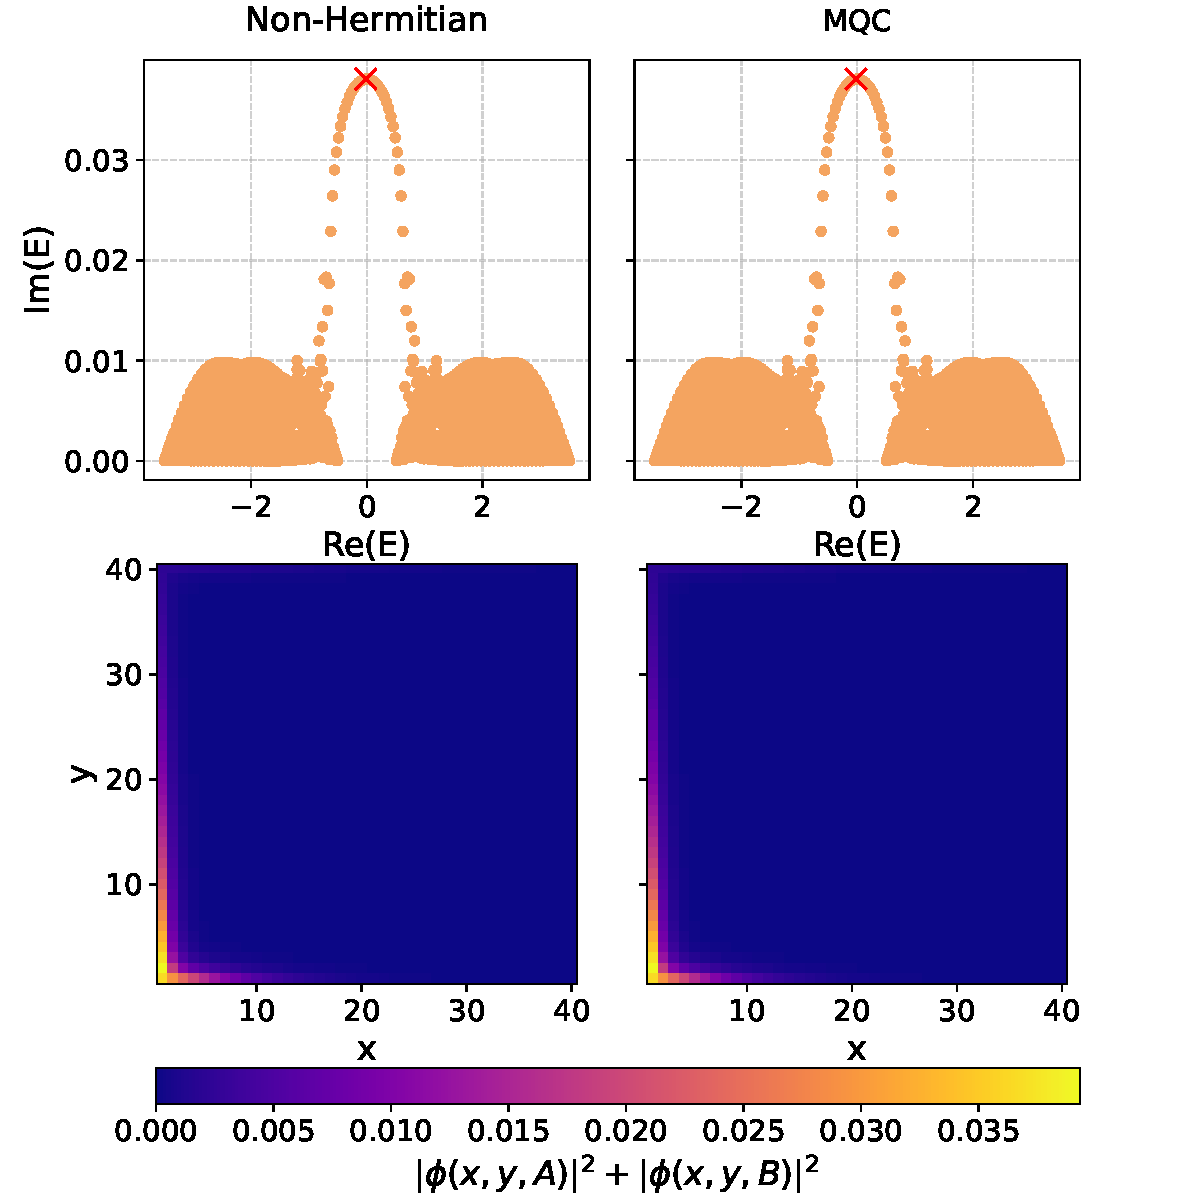
\includegraphics[width=1.\linewidth]{Picture/SingleExcitation_Comp.pdf}
	% 	\caption{在单激发子空间中能谱和本征态对比。(a) 非厄米哈密顿量的能谱和本征态在各元胞的粒子数。 (b) MQC的有效哈密顿量$\hat{H}_{\mathrm{eff}}^{(N)}$的能谱和本征态在各元胞的粒子数。 该本征态是chiral skin mode，其能量在能谱中用红色十字标记。系统尺寸为$L_x=L_y=40$，非厄米参数为$\gamma=0.2$，在位能为$u=-1.5$。MQC的参数为$N=200$, $\mathrm{d}t$=0.001。}
	% 	\label{fig:02}
	% \end{figure} %label from y=1 and x=1?


	% \subsection{Two-excitation subspace}


	\begin{figure*}[htbp]
		\begin{minipage}[b]{0.68\textwidth}
			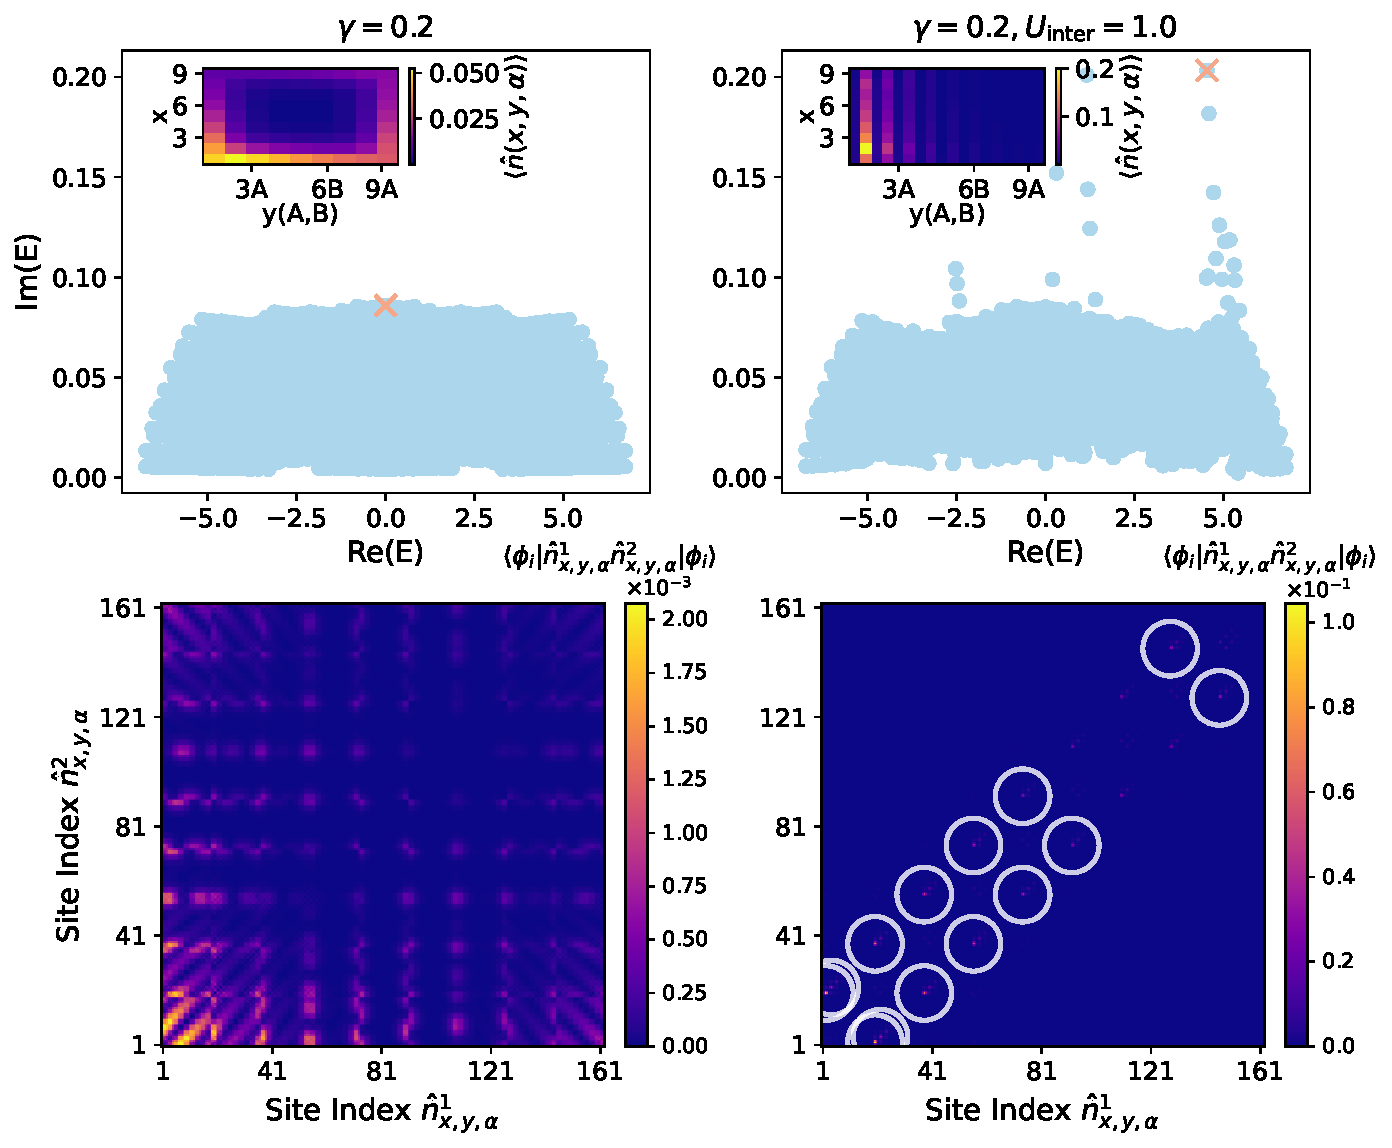
\includegraphics[width=\textwidth]{picture2/Pic_TwoExcitation.pdf}
			% \caption{图片3说明}
			% \label{fig:img3}
		\end{minipage}
		\begin{overpic}[width=0.31\linewidth]{picture2/Mech3.pdf}
			% \put(-98,152){(a1)}
			% \put(-33,152){(a2)}
			% \put(32,152){(a3)}
			% \put(7,54){(c)}
			\put(-128,100){(a1)}
			\put(-64,100){(a2)}
			\put(-128,52){(b1)}
			\put(-64,52){(b2)}
			\put(-3,100){(c)}
			% \put(49,54){(d)}
		\end{overpic}
		\caption{
			(a) The spectrum of non-Hermitian Hamiltonian without interaction and with interaction $\hat{H}_{\text{inter}}$ in two-excitation subspace. 
			The eigenstate's average particle number $\langle \hat{n}(x,y,\alpha) \rangle$ of the eigenstate with the largest imaginary eigenvalue is shown in the inset. The non-Hermitian gain is applied to $y=1$ boundary. The energy of eigenstates is indicated by orange cross in spectrum. 
			(b) The two-particle correlation function $\langle \phi_i \vert \hat{n}^1 \hat{n}^2 \vert \phi_i \rangle$ bwteen two particles of the eigenstate with the largest imaginary eigenvalue for non-Hermitian Hamiltonians with or without many-body interaction. In (b2), the positions where the two-particle correlation function exceeds 0.03 are marked with white circles.
		The system size is $L_x=L_y=9$ and the onsite potential is $u=-1.5$. The non-Hermitian gain is applied to $y=1$ boundary. 
		(c) Schematic representation of quantum states in the two-excitation subspace with and without $\hat{H}_{\text{inter}}$ many-body interaction. 
		Blue spheres: unit cells; blue downward arrows (red upward arrows): particles at $A$ ($B$) sublattice; black arrows: allowed transitions; blue wavy arrows: non-Hermitian pumping (arrow number indicates strength). 
		%Blue sphere represent unit cells and blue downward arrows (red upward arrows) indicate particles at $A$ ($B$) sublattice. 
		%Black arrows represent allowed transitions. Blue wavy arrows indicate non-Hermitian pumping, showing the particle flow to specific quantum states after time evolution. The number of blue wavy arrows represents the strength of the pumping effect. 
		The energy splitting induced by many-body interactions is denoted by $U_{\text{inter}}$.}
		\label{fig:02}
	\end{figure*}

	
	The many-body effect emerges if the excitation is beyond more than one. 
	When investigating many-body systems, whether the chiral skin effect persists in the presence of many-body interactions remains a problem, and the interplay between many-body interactions and non-Hermiticity is still an unresolved question. 
	Considering the commutation between the $\hat{N}$ and $\hat{H}$, the dynamics will be confined within the subspace of the same excitation. When concerning about the two-excitation subspace, the interplay between the many-body interactions and non-Hermiticity can be found. 
	In the two-excitation subspace, the spectrum and average particle number at each lattice site of the gain non-Hermitian Hamiltonians 
	%both in the absence and presence of inter-cell interaction $\hat{H}_{\text{inter}}$ 
	are shown in Fig.~\ref{fig:02}.

	% 但是泡利排斥阻止所有粒子在同一个角落上积累。
	% Fig.~\ref{fig:02} (a)展示了在双激发子空间中每一种非厄米哈密顿量的复能谱，最大虚本征值的本征态，其复能量在能谱中用橘色十字表示。该本征态位于双激发子空间中，其中每个基矢均对应于一个双激发量子态，如图2中的插图所示。同时，在第三行展示了该本征态的在每个格点的平均粒子数，定义为
	% \begin{equation}
	% 	\langle \hat{n}(x,y,\alpha) \rangle = \langle \phi_i \vert \hat{n}_{x,y,\alpha} \vert \phi_i \rangle,
	% \end{equation}
	% 其中$\phi_i$表示在双粒子子空间中的本征态，$\hat{n}_{x,y,\alpha}$ is the number operator at $\alpha$ sublattice of unit cell with position (${x},{y}$)。
	% 当没有相互作用时，多粒子空间的chiral skin mode可以通过单粒子chiral skin mode进行构造。因此多个chiral skin mode构造的多粒子态仍然会呈现出chiral skin effect，如Fig.~\ref{fig:02} (a)第一列所示。
	% %展示了无相互作用下的手性趋肤模式。
	% 当系统存在相互作用$\hat{H}_{\text{intra}}$时，相应的能谱和最大虚本征值的本征态如Fig.~\ref{fig:02} (a)第二列所示。当系统存在相互作用$\hat{H}_{\text{inter}}$时，相应的能谱和最大虚本征值的本征态如Fig.~\ref{fig:02} (a)第三列所示。
	
	Figs.~\ref{fig:02} (a1-a2) show the energy spectrum
	%, the eigenstate with the largest imaginary eigenvalue, and the average particle number of this eigenstate 
	for the non-Hermitian Hamiltonian with or without the many-body Hamiltonian. 
	% The complex energy of this eigenstate is marked with an orange cross in the spectrum. 
	% 这一小段没有中文，
	The eigenvalue distributions of system with many-body interactions $\hat{H}_{\text{inter}}$ are closely related to the symmetry of the Hamiltonian. The 
	symmetry of the spectrum can be understood as follows. For a non-Hermitian Hamiltonian without interactions, the spectrum exhibits symmetry with respect to the line $\Re(E)=0$ in the complex spectrum plane, consistent with results from single-particle subspaces and previous studies~\cite{nakamura2023universal, ma2024non,schindler2023hermitian}. 
	This symmetry arises because $\hat{H}_{\text{QWZ}}$ and $\hat{H}_{\text{im}}$ possess the anti-$\mathcal{PT}$ symmetry.
	% The interaction Hamiltonian $\hat{H}_{\text{inter}}$ are invariant under a combination of parity ($\mathcal{P}$) and time-reversal ($\mathcal{T}$) operations
	% \begin{equation}
	% 	\begin{split}
	% 		\mathcal{PT} \hat{H}_{\text{inter}} (\mathcal{PT})^{-1} &= \hat{H}_{\text{inter}}
	% 	\end{split}
	% \end{equation}
	% For systems with anti-$\mathcal{PT}$ symmetry, if $\ket{\phi}$ is an eigenstate with energy $E$, there exists another eigenstate $(\mathcal{PT})^{-1} \ket{\phi}$ with energy $-E^*$. 
	The detailed analysis is provided in Appendix~\ref{sec:symmetry_Hamiltonian}.
	%Furthermore, under the $\mathcal{PT}$ transformation, the Hamiltonian $\hat{H}_{\text{inter}}$ with interaction strength $U_{\text{inter}}$ transforms into the Hamiltonian $\hat{H}_{\text{inter}}$ with interaction strength $-U_{\text{inter}}$.

	% In Figs.~\ref{fig:02} (b1-b3), the probability distributions of the eigenstate with the largest imaginary eigenvalue (orange cross in the corresponding Figs.~\ref{fig:02} (a1-a3)) are shown. Here, the  
	% basis in the two-excitation subspace (the label of the $x$ axis in Fig.~\ref{fig:02} (b1-b3)) is
	% \begin{equation}
	% 	\begin{split}
	% 		\{\ket{(11)_{1,1}(00)_{1,2}\cdots}, \ket{(10)_{1,1}(10)_{1,2}\cdots}, \\
	% 		\ket{(01)_{1,1}(10)_{1,2}\cdots},\cdots\},
	% 	\end{split}
	% \end{equation}
	% which represent all possible configurations of two fermions in the system. These basis vectors are arranged in descending order according to the binary representation, which corresponds to the basis states.
	% For example, basis $\ket{(11)_{1,1}(00)_{1,2}(00)_{1,3}\cdots}$ is labeled as basis 1, and basis $\ket{(10)_{1,1}(10)_{1,2}(00)_{1,3}\cdots}$ is labeled as basis 2. 
	% Throughout this work, the notation $\ket{(ab)_{x,y}}$ indicates fermion occupation at the unit cell with position $(x,y)$, where $a=1(0)$ denotes the presence (absence) of fermion at $A$ sublattice and  of $b=1(0)$ denotes the presence (absence) of fermion at $B$ sublattice. 
	% Basis 1 is shown in the inset of Fig.~\ref{fig:02} (b). The eigenstates in the two-excitation subspace are expressed as 
	% \begin{equation}
	% 	\begin{split}
	% 		\phi_i =& a_1 \ket{(11)_{1,1}(00)_{1,2}\cdots} + a_2 \ket{(10)_{1,1}(10)_{1,2}\cdots} + \\
	% 		&a_3 \ket{(01)_{1,1}(10)_{1,2}} + \cdots\\
	% 		=& a_1 \hat{c}_{1,1,A}^{\dagger}\hat{c}_{1,1,B}^{\dagger} \ket{0\cdots} + a_2 \hat{c}_{1,1,A}^{\dagger}\hat{c}_{1,2,A}^{\dagger} \ket{0\cdots} + \\
	% 		& a_3 \hat{c}_{1,1,B}^{\dagger}\hat{c}_{1,2,A}^{\dagger} \ket{0\cdots} + \cdots.
	% 	\end{split}
	% \end{equation}
	%
	%The eigenstate lies in the two-excitation subspace, and each basis of this subspace corresponds to a two-particle quantum state, as shown in the inset of Fig.~\ref{fig:03} (a).  
	The inset of the Figs.~\ref{fig:02} (a1-a2) shows the average particle number at each lattice site for the eigenstate, defined as follows:
	\begin{equation}
		\langle \hat{n}(x,y,\alpha) \rangle = \langle \phi_i \vert \hat{n}_{x,y,\alpha} \vert \phi_i \rangle,
	\end{equation}
	where 
	%$\phi_i$ is eigenstate in two-excitation subspace, 
	$\hat{n}_{x,y,\alpha}$ is number operator at sublattice $\alpha (\alpha=A,B)$ of unit cell $(x,y)$.
	The eigenstate $\vert \phi_i \rangle$ is the eigenstate the largest imaginary eigenvalue (orange cross in the corresponding Figs.~\ref{fig:02} (a1-a2)). The eigenstates in the two-excitation subspace are expressed as 
	\begin{equation}
		\begin{split}
			\phi_i =& a_1 \ket{(11)_{1,1}(00)_{1,2}\cdots} + a_2 \ket{(10)_{1,1}(10)_{1,2}\cdots} + \\
			&a_3 \ket{(01)_{1,1}(10)_{1,2}} + \cdots\\
			=& a_1 \hat{c}_{1,1,A}^{\dagger}\hat{c}_{1,1,B}^{\dagger} \ket{0\cdots} + a_2 \hat{c}_{1,1,A}^{\dagger}\hat{c}_{1,2,A}^{\dagger} \ket{0\cdots} + \\
			& a_3 \hat{c}_{1,1,B}^{\dagger}\hat{c}_{1,2,A}^{\dagger} \ket{0\cdots} + \cdots.
		\end{split}
	\end{equation}
	Throughout this work, the notation $\ket{(ab)_{x,y}}$ indicates fermion occupation at the unit cell with position $(x,y)$, where $a=1(0)$ denotes the presence (absence) of fermion at $A$ sublattice and $b=1(0)$ denotes the presence (absence) of fermion at $B$ sublattice.
	In the absence of interaction, the multi-particle chiral skin modes can be constructed from single-particle chiral skin modes. Consequently, multi-particle states formed by these modes still preserve the characteristic of the chiral skin effect, as shown in the inset of Fig.~\ref{fig:02}(a1).
	%, which demonstrates the chiral skin modes in the absence of interaction.
	% When many-body interaction $\hat{H}_{\text{intra}}$ is introduced, the energy spectrum and eigenstates with the largest imaginary eigenvalues are shown in Figs.\ref{fig:02}(a2) and (b2). Under the intra-cell interaction $\hat{H}_{\text{intra}}$ ($U_{\text{intra}}=1.0$), the spectrum of the Hamiltonian in the two-excitation subspace shows that although the symmetry of the spectrum with respect to $\mathrm{Re}(E)=0$ is broken, the eigenstate with the largest imaginary eigenvalue retains a chiral skin mode. The difference exists solely in the particle number occupation at each lattice site. In contrast, 
	When many-body interaction $\hat{H}_{\text{inter}}$ is introduced, the results are shown in the Figs.\ref{fig:02}(a2). The many-body interaction $\hat{H}_{\text{inter}}$($U_{\text{inter}}=1.0$) alters eigenvalue distribution and eigenstate localization pattern. 

	% The horizontal axis represents different basis, and each basis corresponds to a three-particle quantum state, as shown in the inset of Fig.\ref{fig:03}(a). 

	% %%%%% 这一段应该删除，没有细节没有意义。
	% 在单粒子子空间中，量子态的局域化直接反映粒子数算符的分布特征，这源于单粒子空间的每一个基矢对应一个格点的激发。然而，在双粒子激发子空间（如图~\ref{fig:02}(a)所示），量子态局域化与粒子数分布呈现非平庸对应关系。通过计算具有最大虚本征值的本征态的平均粒子数$\langle \hat{n}(x,y,\alpha) \rangle$，我们发现：在无相互作用时($\gamma=0.2$)，两粒子手征趋肤模仍保持corner局域特征，其空间分布模式与单粒子情形相似（见图~\ref{fig:02}(a)第一列）；但当引入相互作用后，粒子数分布和本征态分布展现出新的特征（见图~\ref{fig:02} (a)右）。
	% % 出现这一现象的原因在于，
	% %之所以此时粒子数并不是两个单粒子chiral skin mode的粒子数之和是由于泡利排斥原理。


	% % 在元胞内相互作用$\hat{H}_{\text{intra}}$($U_{\text{intra}}=1.0$)作用下,在双激发子空间中对哈密顿量的能谱显示，虽然复能谱的$\mathrm{Re}(E)=0$对称性破缺，但最大虚本征态仍维持corner state形态，仅每个格点的粒子数占据有所区别。相反地，元胞间相互作用$\hat{H}_{\text{inter}}$($U_{\text{inter}}=1.0$)引发显著能谱重构。
	
	% Under the intra-cell interaction $\hat{H}_{\text{intra}}$ ($U_{\text{intra}}=1.0$), the spectrum of the Hamiltonian in the two-excitation subspace shows that although the symmetry of the spectrum with respect to $\mathrm{Re}(E)=0$ is broken, the eigenstate with the largest imaginary eigenvalue retains chiral skin mode. 
	% The difference exists solely in the particle number occupation at each lattice site. In contrast, the many-body interaction $\hat{H}_{\text{inter}}$($U_{\text{inter}}=1.0$) alters eigenvalue distribution and eigenstate localization pattern. 


	% 对于不存在相互作用的非厄米哈密顿量，其本征能谱是关于复能谱中$\Re(E)=0$的直线对称的，这与单粒子子空间的结果以及以前的研究结果一致。这种对称性可以归因于$\hat{H}_{\text{QWZ}}$是在宇称和时间反演对称变换下反号，也就是anti-$\mathcal{PT}$对称的。另一方面非厄米哈密顿量$\hat{H}_{\text{im}}$在宇称变换下保持不变，但是在时间反演对称变换下反号$-\hat{H}_{\text{im}}$，因此，$\hat{H}_{\text{im}}$同样具有anti-$\mathcal{PT}$对称性，也就是
	% \begin{equation}
	% 	\begin{split}
	% 		\mathcal{PT} \hat{H}_{\text{QWZ}} (\mathcal{PT})^{-1} = -\hat{H}_{\text{QWZ}} \\
	% 		\mathcal{PT} \hat{H}_{\text{im}} (\mathcal{PT})^{-1} = -\hat{H}_{\text{im}}.
	% 	\end{split}
	% \end{equation}
	% 然而，相互作用哈密顿量$\hat{H}_{\text{inter}}$和$\hat{H}_{\text{intra}}$ are invariant under a combination of parity ($\mathcal{P}$) and time-reversal ($\mathcal{T}$) operations
	% \begin{equation}
	% 	\begin{split}
	% 		\mathcal{PT} \hat{H}_{\text{inter}} (\mathcal{PT})^{-1} = \hat{H}_{\text{inter}}% \\
	% 		% \mathcal{PT} \hat{H}_{\text{intra}} (\mathcal{PT})^{-1} = \hat{H}_{\text{intra}}.
	% 	\end{split}
	% \end{equation}
	% 对于存在anti-$\mathcal{PT}$ symmetry的系统，它的能谱是关于复能谱的$\Re(E)=0$直线对称的，这是因为
	% \begin{equation}
	% 	\begin{split}
	% 		\hat{H} \vert \phi \rangle = E \vert \phi \rangle\\
	% 		\mathcal{PT} \hat{H} (\mathcal{PT})^{-1} \vert \phi \rangle = - E \vert \phi \rangle\\
	% 		\hat{H} (\mathcal{PT})^{-1} \vert \phi \rangle = - E^* (\mathcal{PT})^{-1} \vert \phi \rangle.
	% 	\end{split}
	% \end{equation}
	% 这表明，如果$\vert \phi \rangle$是能量为$E$的本征态，那么对于具有anti-$\mathcal{PT}$ symmetry的系统，它也存在能量为$-E^*$的本征态$(\mathcal{PT})^{-1} \vert \phi \rangle$，因此，系统的能谱是关于复能谱的$\Re(E)=0$直线对称的。
	% 此外，在$\mathcal{PT}$变换下，相互作用强度为$U_{\text{inter}}$的$\hat{H}_{\text{inter}}$将变换为相互作用强度为$-U_{\text{inter}}$的$\hat{H}_{\text{inter}}$。
	% %和$\hat{H}_{\text{intra}}$
	% 因此，具有相互作用强度为$U_{\text{inter}}$的多体哈密顿量的能谱和本征态与相互作用为$-U_{\text{inter}}$的多体哈密顿量的能谱和本征态之间存在对称性
	% \begin{equation}
	% 	\begin{split}
	% 		\mathcal{PT} (\hat{H}_{\text{QWZ}}+\hat{H}_{\text{inter}}\vert_{U_{\text{inter}}}+\hat{H}_{\text{im}}) (\mathcal{PT})^{-1}\\
	% 		= -(\hat{H}_{\text{QWZ}}+\hat{H}_{\text{inter}}\vert_{-U_{\text{inter}}}+\hat{H}_{\text{im}}).
	% 	\end{split}
	% \end{equation}
	% 相互作用$U_{\text{inter}}$的系统的本征值和本征态分别为可以表示为$\{E_{\text{inter}}\}$和$\{\phi_{\text{inter}}\}$，相互作用$-U_{\text{inter}}$的系统的本征值和本征态则为$\{-E^*_{\text{inter}}\}$和$\{(\mathcal{PT})\phi_{\text{inter}}\}$。


	% This symmetry arises because $\hat{H}_{\text{QWZ}}$ change sign under a combination of parity and time-reversal transformations, and this symmetry is called anti-$\mathcal{PT}$ symmetry. On the other hand, the non-Hermitian Hamiltonian $\hat{H}_{\text{im}}$ remains invariant under parity transformation but changes sign under time-reversal transformation, thus also exhibiting anti-$\mathcal{PT}$ symmetry
	% \begin{equation}
	% 	\begin{split}
	% 		\mathcal{PT} \hat{H}_{\text{QWZ}} (\mathcal{PT})^{-1} &= -\hat{H}_{\text{QWZ}} \\
	% 		\mathcal{PT} \hat{H}_{\text{im}} (\mathcal{PT})^{-1} &= -\hat{H}_{\text{im}}.
	% 	\end{split}
	% \end{equation}
	% However, the interaction Hamiltonian $\hat{H}_{\text{inter}}$ and $\hat{H}_{\text{intra}}$ are invariant under a combination of parity ($\mathcal{P}$) and time-reversal ($\mathcal{T}$) operations
	% \begin{equation}
	% 	\begin{split}
	% 		\mathcal{PT} \hat{H}_{\text{inter}} (\mathcal{PT})^{-1} = \hat{H}_{\text{inter}}% \\
	% 		% \mathcal{PT} \hat{H}_{\text{intra}} (\mathcal{PT})^{-1} = \hat{H}_{\text{intra}}.
	% 	\end{split}
	% \end{equation}
	% For systems with anti-$\mathcal{PT}$ symmetry, the energy spectrum is symmetric with respect to the line $\Re(E)=0$ in the complex energy plane, because
	% \begin{equation}
	% 	\begin{split}
	% 		\hat{H} \vert \phi \rangle &= E \vert \phi \rangle\\
	% 		\mathcal{PT} \hat{H} (\mathcal{PT})^{-1} \vert \phi \rangle &= - E \vert \phi \rangle\\
	% 		\hat{H} (\mathcal{PT})^{-1} \vert \phi \rangle &= - E^* (\mathcal{PT})^{-1} \vert \phi \rangle.
	% 	\end{split}
	% \end{equation}
	% This demonstrates that for a system with anti-$\mathcal{PT}$ symmetry, if $\ket{\phi}$ is an eigenstate with energy $E$, there exists another eigenstate $(\mathcal{PT})^{-1} \ket{\phi}$ with energy $-E^*$. Consequently, the energy spectrum of the system is symmetric with respect to the line $\Re(E)=0$ in the energy plane.
	% Furthermore, under the $\mathcal{PT}$ transformation, the Hamiltonian $\hat{H}_{\text{inter}}$ with interaction strength $U_{\text{inter}}$ transforms into the Hamiltonian $\hat{H}_{\text{inter}}$ with interaction strength $-U_{\text{inter}}$. Consequently, the energy spectrum and eigenstates of the many-body Hamiltonian with interaction strength $U_{\text{inter}}$ demonstrate a symmetric relationship with those of the Hamiltonian with interaction strength $-U_{\text{inter}}$
	% \begin{equation}
	% 	\begin{split}
	% 		\mathcal{PT} (\hat{H}_{\text{QWZ}}+\hat{H}_{\text{inter}}\vert_{U_{\text{inter}}}+\hat{H}_{\text{im}}) (\mathcal{PT})^{-1}\\
	% 		= -(\hat{H}_{\text{QWZ}}+\hat{H}_{\text{inter}}\vert_{-U_{\text{inter}}}+\hat{H}_{\text{im}}).
	% 	\end{split}
	% \end{equation}
	% The eigenvalues and eigenstates of the Hamiltonians with interaction strength $U_{\text{inter}}$ are denoted as $\{E_{\text{inter}}\}$ and $\{\phi_{\text{inter}}\}$, respectively. For the Hamiltonians with interaction strength $-U_{\text{inter}}$, the eigenvalues and eigenstates are $\{E_{\text{inter}}^*\}$ and $\{(\mathcal{PT})\phi_{\text{inter}}\}$, respectively.

	% 多体相互作用的引入导致本征态呈超局域特征——本征态局域在部分两粒子态上，这些态的两个粒子的$x$坐标为$(x_1,x_2)=(1,2),...,(8,9)$，$y$坐标为$y=1$，并且位于B子格点上(见图~\ref{fig:02}(a)第三列)。


	% 这一现象的物理机制源于双重竞争效应：手征趋肤效应驱动粒子向系统corner聚集，而多体相互作用通过诱导能级差($\Delta E \propto U_{\text{inter}}\langle n_i n_j \rangle$)抑制粒子从耗散格点($y=1$)向非耗散格点($y\geq2$)的跃迁。
	% 从Fig.~\ref{fig:02}(a)中发现当不存在相互作用和相互作用为$\hat{H}_{\text{intra}}$时，本征态在双激发子空间中表现出局域化特征，而当存在相互作用$\hat{H}_{\text{inter}}$时，量子态在特定基矢上的概率幅呈现显著增强的局域化分布特性，可以看出该hybrid chiral skin correlated states比chiral skin mode局域化得多。
	%在不存在chiral skin mode的情况下，具有较大虚部的本征态尽管属于bulk state，但其粒子分布更接近耗散格点。当引入多体相互作用时，这些相互作用不仅增强了量子态的局域性，还导致量子态在不同子格点上的权重重新分配。这一现象揭示了多体相互作用在调控量子态空间分布中的重要作用，为理解非厄米系统中的拓扑特性提供了新的视角。
	% 本征态的展宽

	
	The introduction of many-body interaction resulting in the super-localization of eigenstates can also be understood from the two-particle correlation function. 
	% The many-body interaction alters the spatial distribution of chiral skin mode, revealing the interaction mechanism between chiral skin modes and many-body interactions in non-Hermitian many-body systems. 
	% Specifically, these eigenstates are localized on specific two-particle configuration. 
	We show the two-particle correlation function $\langle \phi_i \vert \hat{n}^1_{x,y,\alpha} \hat{n}^2_{x,y,\alpha} \vert \phi_i \rangle$ for the eigenstate with the largest imaginary eigenvalue in Fig.~\ref{fig:02} (b1-b2). The operator $\hat{n}^1_{x,y,\alpha}$ ($\hat{n}^2_{x,y,\alpha}$) is the number operator of the first (second) particle at the $\alpha$ sublattice of the unit cell $(x,y)$.
	% The correlation patterns remain qualitatively similar between the non-interacting case and intra-cell interaction case. 
	% The results show that the two-particle correlation function in the absence of interaction and in the presence of interaction $\hat{H}_{\text{intra}}$ is similar. 
	For the inter-cell interaction case, the two-particle correlation function reveals strong spatial correlation between the location of two particles. 
	In Figs.\ref{fig:02}(b1), the correlation function is of the order of $10^{-3}$, while it reaches approximately $10^{-1}$ in Fig.\ref{fig:02}(b2). Locations where the two-particle correlation function exceeds $0.03$ are indicated by white circles in Fig.~\ref{fig:02}(b2).
	Particles preferentially occupy adjacent sites ($\Delta x =1$) along $y=1$.  The particles are also more localized on sublattice $B$. 
	% The two-particle correlation function in the presence of interaction $\hat{H}_{\text{inter}}$ suggests a strong correlation between the location of two particles. The $y$ coordinate of two particles are the same, and the $x$ coordinate of two particles are next to each other. The particles are more localized on sublattice $B$. 
	% Specifically, these eigenstates are localized on specific two-particle configuration where the $x$ coordinates of the two particles are $(x_1,x_2)=(1,2),...,(8,9)$ and the $y$ coordinate is $y=1$. These states show the particles are more localized on sublattice B (see the third column of Fig.~\ref{fig:02}(a)).
	For the strong correlation emerges in the localized state in Fig.~\ref{fig:02}(b2), such localized states are called as hybrid chiral skin correlated states, which are much localized compared to the conventional chiral skin modes.
	%This reveals that the hybrid chiral skin correlated states are much more localized compared to the chiral skin mode.
	% In the absence of chiral skin mode, eigenstates with larger imaginary parts, despite being classified as bulk states, exhibit particle distributions that are more concentrated near dissipative lattice sites. When multi-body interactions are introduced, these interactions not only enhance the localization of quantum states but also lead to a redistribution of quantum state weights across sublattice sites. This phenomenon highlights the crucial role of multi-body interactions in regulating the spatial distribution of quantum states, offering new insights into the topological properties of non-Hermitian systems.

	% 值得注意的是，尽管相互作用体系的本征态呈现超局域特征，但是其粒子数算符均值仍然显示出相似之处，它们都局域在左下角，多体相互作用使chiral skin的粒子进行了重新分布。这揭示了非厄米多体系统中chiral skin mode与多体相互作用的协同作用机制。

	% Notably, the eigenstates of the interacting system show super-localized characteristics. 
	% %The expectation values of the particle number operator still share similarities, as they are localized in the lower-left corner. 
	% The many-body interactions lead to the redistribution of chiral skin mode, revealing the interaction mechanism between chiral skin modes and many-body interactions in non-Hermitian many-body systems.

	% % !!!这里无论如何要点出我们是从演化角度考虑的。
	% 接下来，我们说明，Fig.~\ref{fig:02}中的hybrid chiral skin-many body是由chiral skin effect和相互作用共同作用的结果。该机理可以通过非厄米哈密顿量的时间演化来理解。% 这需要说明与chiral skin不同，还是说明不仅是由非厄米共同导致的。
	% 在Fig.~\ref{fig:02} (b)中，我们给出了不同相互作用下，仅考虑三个元胞且仅有两个粒子时的部分能级，其中蓝色波浪线表示非厄米pumping，该泵浦仅作用于前两个元胞，黑色箭头表示可能发生的跃迁，所有可能的跃迁振幅大小为$1/2$。我们在这里用$\ket{\uparrow}$表示在元胞的$B$子格点有一个粒子；用$\ket{\downarrow}$表示在元胞的$A$子格点有一个粒子(此时$u<0$，位于$B$格点的粒子能量更高)。如果在Fig.~\ref{fig:02} (b)中的某个蓝色元胞同时存在$\ket{\uparrow}$和$\ket{\downarrow}$，则表示该元胞的$A$格点和$B$格点各有一个粒子。

	% % !!!这里无论如何要点出我们是从演化角度考虑的。
	The emergence of hybrid chiral skin correlated states arises from a competitive mechanism: the chiral skin effect drives particles to accumulate at the corners of the system, while many-body interactions suppress particle transitions from unit cells with gain ($y=1$) to unit cells without gain ($y \geq 2$) by inducing energy level splitting ($\Delta E \propto U_{\text{inter}}\langle n_i n_j \rangle$), thereby influencing the system's topological properties.
	As shown in the inset of Fig.~\ref{fig:02}(a1), eigenstates in the two-excitation subspace exhibit localized characteristics 
	without many-body interaction (inset of Fig.~\ref{fig:02} (a1)). However, in the presence of interaction $\hat{H}_{\text{inter}}$, eigenstates display significantly enhanced localization, and probability amplitudes are concentrated on specific basis states, such as $\ket{(01)_{1,1}(01)_{1,2}(00)_{1,3}\cdots}$, as shown in the inset of Fig.~\ref{fig:02} (a2). 

	The above mechanism of generating such hybrid chiral skin correlated states can also be analyzed with the aid of Fock space representation, as illustrated in Fig.~\ref{fig:02}(c). 
	To achieve a more compact presentation of Fig.~\ref{fig:02}(c), unit cells with gain ($\forall x$ and $y$ = 1) are arranged first, followed by those without gain.
	The underlying mechanism can be understood in terms of the time evolution governed by a non-Hermitian Hamiltonian. 
	We focus on the state with the two particles located at the positions $(x,y)=(1,1), (1,2)$ and $(2,1)$.
	%We analyze a minimal system comprising three unit cells located at $(x,y)=(2,1),(1,1),(1,2)$, and there are two particles in the system. The energy spectrum of this system is show in Fig.~\ref{fig:02_Supple} (b). 
	% 没有按照顺序排列，需要在这里说吗？
	% As a paradigmatic example, Fig.~\ref{fig:02}(d) displays the energy levels of a minimal system with three unit cells and two particles under different interactions.
	%In Fig.~\ref{fig:02}(b), we present energy levels for a system with three unit cells and two particles under different interaction as an example.
	The symbols in Fig.~\ref{fig:02_Supple}(b) is explained as follows:
	\begin{enumerate}
		\item In Fig.~\ref{fig:02}(c), $\ket{\uparrow}$ represents a particle at the higher-energy $B$ sublattice (when $u<0$), while $\ket{\downarrow}$ represents a particle at the $A$ sublattice of the unit cell. 
		Blue spheres represent the unit cells. 
		% A particle at the B sublattice of the unit cell is represented by $\ket{\uparrow}$ (when $u<0$, the particle at B sublattice possesses higher energy). A particle at the A sublattice of the unit cell is represented by $\ket{\uparrow}$.
		Notably, when both $\ket{\uparrow}$ and $\ket{\downarrow}$ coexist in a unit cell (blue sphere), it indicates one particle is located at the $A$ sublattice and the other is located at the $B$ sublattice. 
		\item The blue wavy lines denote the non-Hermitian pumping governed by $\hat{H}_{\text{im}}$, which is restricted to the first two unit cells. Under time evolution, because the gain in $\hat{H}_{\text{im}}$ are applied to the unit cells along $y=1$ boundary, the quantum state amplitudes undergo exponential amplification proportional to their occupation number at the first two unit cells before normalization. For instance, the state $a_1 \ket{(01)_{1,1}(01)_{2,1}\cdots(00)_{1,2}\cdots} + a_2\ket{(00)_{1,1}(01)_{2,1}\cdots(01)_{1,2}\cdots}$ evolves under time $\mathrm{d}t$ to state $a_1 e^{2\gamma \mathrm{d}t} \ket{(01)_{1,1}(01)_{2,1}\cdots(00)_{1,2}\cdots} + a_2 e^{\gamma \mathrm{d}t} \ket{(00)_{1,1}(01)_{2,1}\cdots(01)_{1,2}\cdots}$ before normalization, where the exponents reflect the pumping strength. 
		% 解释为什么没有按照增加x坐标来描述元胞的位置。
		%Note that the unit cells in the state $\ket{(01)_{1,1}(01)_{2,1}\cdots(00)_{1,2}\cdots}$ is not arranged in order of increasing $x$-coordinate for this minimal system.
		\item Black arrows indicate the hopping term in $\hat{H}_{\text{QWZ}}$, and the magnitude of the transition amplitude is $1/2$. 
		\item The vertical axis quantifies the total energy, comprising contributions from both the onsite energy ($u=-1.5$) in $\hat{H}_{\text{QWZ}}$ and the many-body interaction. For $\hat{H}_{\text{inter}}$ interaction, the energy of state $\ket{(01)_{1,1}(01)_{2,1}\cdots(00)_{1,2}\cdots}$ is $E=-2u+U_{\text{inter}}=4$, and the energy of the state $\ket{(00)_{1,1}(01)_{2,1}\cdots(10)_{1,2}\cdots}$ is $E=-u+u=0$. 
	\end{enumerate}

	% 对于非厄米哈密顿量，量子态的能量等于每一个粒子的能量之和(Fig.~\ref{fig:02}(b))。此时，非厄米pumping会将粒子pump到子空间
	% \begin{equation}
	% 	\mathscr{H}_{\text{gain}}=\left\{ \ket{\uparrow\uparrow0}, \ket{\downarrow\downarrow0},\ket{\uparrow\downarrow0},\ket{\downarrow\uparrow0},\ket{\underline{\uparrow\downarrow}00},\ket{0\underline{\uparrow\downarrow}0}\right\}.
	% \end{equation}
	% 根据非厄米项的时间演化$e^{-\mathrm{i}\hat{H}_{\text{im}} \mathrm{d}t}$，当粒子所在的两个元胞均存在增益时，这些量子态受到的增益更强。泵入空间$\mathscr{H}_{\text{gain}}$的每个量子态的强度与其概率幅成正比。在不存在多体相互作用时，$\mathscr{H}_{\text{gain}}$中的量子态与其他空间中的量子态无能量差，导致大部分粒子通过跃迁离开$\mathscr{H}_{\text{gain}}$，从而引发chiral skin effect。量子态在非厄米哈密顿量的时间演化后，进一步演化为chiral skin mode。
	When concerning with the second key point above,
	%, for a non-Hermitian Hamiltonian, the energy of each state equals to the summation of individual particle's onsite energy, as shown in Fig.~\ref{fig:02_Supple}(b). 
	the non-Hermitian evolution drives the particles into the specific subspace
	\begin{equation}
		\begin{split}
			% \mathscr{H}_{\text{gain}}=\left\{ \ket{\uparrow\uparrow0}, \ket{\downarrow\downarrow0},\ket{\uparrow\downarrow0},\ket{\downarrow\uparrow0},\ket{\underline{\uparrow\downarrow}00},\ket{0\underline{\uparrow\downarrow}0}\right\}.
			\mathscr{H}_{\text{gain}}=\left\{ \ket{(01)_{1,1}(01)_{2,1}\cdots(00)_{1,2}\cdots}, \right.\\
			\ket{(10)_{1,1}(10)_{2,1}\cdots(00)_{1,2}\cdots},  \\
			\ket{(01)_{1,1}(10)_{2,1}\cdots(00)_{1,2}\cdots},\\
			\ket{(10)_{1,1}(01)_{2,1}\cdots(00)_{1,2}\cdots},\\
			\ket{(11)_{1,1}(00)_{2,1}\cdots(00)_{1,2}\cdots},\\
			\left.\ket{(00)_{1,1}(11)_{2,1}\cdots(00)_{1,2}\cdots}, \cdots \right\},
		\end{split}
	\end{equation}
	where both particles are at the $y=1$ boundary.
	Under the time evolution governed by the non-Hermitian term $e^{-\mathrm{i}\hat{H}_{\text{im}} \mathrm{d}t}$, when both sites occupied by the fermions exhibit gain, these quantum states experience stronger gain. 
	The pumping effeciency into the subspace $\mathscr{H}_{\text{gain}}$ 
	scale with the overlap of quantum states with the subspace $\mathscr{H}_{\text{gain}}$. 
	%is proportional to the probability amplitude of each state within this subspace. 
	In the absence of many-body interaction, the 'energy degeneracy' between states inside and outside the Hilbert space $\mathscr{H}_{\text{gain}}$ allows significant particle leakage from this subspace.
	%there is no energy difference between the states within $\mathscr{H}_{\text{gain}}$ and those outside of it, leading to a significant portion of the particles jump out of $\mathscr{H}_{\text{gain}}$. 
	Through continued non-Hermitian evolution, these quantum states ultimately evolve into chiral skin modes.
	% Quantum states further evolve into chiral skin modes under the time evolution of the non-Hermitian Hamiltonian.
	% 这一个应该往chiral skin mode上去靠。
	% For the non-Hermitian Hamiltonians with many-body interaction $\hat{H}_{\text{intra}}$, the localized states are similar to chiral skin modes. 
	% This similarity arises because the many-body interaction $\hat{H}_{\text{intra}}$ does not break the 'energy degeneracy' between states inside and outside $\mathscr{H}_{\text{gain}}$. It results in localization patterns similar to the non-interacting case where only chiral skin modes are observable (Fig.~\ref{fig:02} (c2)).
	%This similarity arises because the energy levels within $\mathscr{H}_{\text{gain}}$ possess the same energy with those outside $\mathscr{H}_{\text{gain}}$ which can be jumped to. Consequently, only the chiral skin effect can be observed in this scenario (Fig.~\ref{fig:02}).

	% 当存在多体相互作用时，非厄米pumping同样会将粒子pump到空间$\mathscr{H}_{\text{gain}}$中的量子态，然而，在存在多体相互作用$\hat{H}_{\text{inter}}$时，该空间中的量子态与能跃迁到的其它能级之间至少存在$U$的能级差，因此被pump到该空间的粒子跃迁到该空间之外的几率更低，从而导致局域化现象的出现。
	% 与存在多体相互作用$\hat{H}_{\text{inter}}$时不同，不存在$\hat{H}_{\text{inter}}$时出现的是一种非厄米拓扑效应，这种效应仅在QWZ模型是拓扑绝缘体时才会存在，即当$-2<u<0$和$0<u<2$。然而，由增益/耗散和多体相互作用共同作用引起的多体局域化现象并不依赖于拓扑绝缘体的存在，相关讨论已在Appendix.~\ref{sec:NHMBL}中进行详细阐述。因此，这两种局域化现象的机制是完全不同的。对于含元胞内多体相互作用的非厄米哈密顿量
	% \begin{equation}
	% 	\hat{H}_{\text{intra}} = \sum_{{x}=1}^{L_{x}-1} \sum_{{y}=1}^{L_{y}}  U_{\text{intra}} \hat{n}_{{x}, {y}, A} \hat{n}_{{x}, {y}, B},
	% \end{equation}
	% where $U_{\text{intra}}$ is the interaction strength. 
	% 此时多粒子空间的局域态与不存在多体相互作用时类似，$\mathscr{H}_{\text{gain}}$中的部分能级与能跃迁到的能级之间不存在能级差，因此在这种多体相互作用的非厄米哈密顿量下，同样只可能观察到chiral skin effect，相关讨论已在Appendix.~\ref{sec:NHMBL_intra}中详细阐述。

	% 当存在多体相互作用时，非厄米pumping同样会将粒子pump到chiral skin mode上。
	% %然而，在存在多体相互作用$\hat{H}_{\text{inter}}$时，被pump到耗散格点的粒子与能跃迁到的邻近非耗散格点之间存在$\vert U \vert$的能级差，因此粒子跃迁到非耗散格点之外的几率更低，从而导致局域化现象的出现。
	% % 与存在多体相互作用$\hat{H}_{\text{inter}}$时不同，不存在$\hat{H}_{\text{inter}}$时出现的是一种非厄米拓扑效应，这种效应仅在QWZ模型是拓扑绝缘体时才会存在，即当$-2<u<0$和$0<u<2$。然而，由增益/耗散和多体相互作用共同作用引起的多体局域化现象并不依赖于拓扑绝缘体的存在，相关讨论已在Appendix.~\ref{sec:NHMBL}中进行详细阐述。因此，这两种局域化现象的机制是完全不同的。对于含元胞内多体相互作用的非厄米哈密顿量
	% 当存在多体相互作用$\hat{H}_{\text{inter}}$时，由于能级差$\vert U \vert$，跃迁到$\hat{H}_{\text{inter}}$外的几率更低，从而导致局域化现象。
	% 不存在相互作用$\hat{H}_{\text{inter}}$时的chiral skin mode是一种单粒子拓扑效应，存在相互作用时的hybrid chiral skin-many body induced localized由拓扑量子态和多体相互作用共同导致的。我们在附录~\ref{sec:NHMBL}中给出了仅由增益/耗散和多体相互作用共同导致的局域态，这两种局域化机制完全不同。
	% 对于含元胞内多体相互作用$\hat{H}_{\text{intra}}$的非厄米哈密顿量，多粒子空间的局域态与无多体相互作用时类似，由于$\mathscr{H}_{\text{gain}}$中的部分能级与可跃迁的能级间不存在能级差，因此在这种情况下仅能观察到chiral skin effect（如图~\ref{fig:02}所示）。
	% % 对于含元胞内多体相互作用的非厄米哈密顿量$\hat{H}_{\text{intra}}$此时多粒子空间的局域态与不存在多体相互作用时类似，$\mathscr{H}_{\text{gain}}$中的部分能级与能跃迁到的能级之间不存在能级差，因此在这种多体相互作用的非厄米哈密顿量下，同样只可能观察到chiral skin effect(Fig.~\ref{fig:02})。
	% %，相关讨论已在Appendix.~\ref{sec:NHMBL_intra}中详细阐述。

	% When many-body interactions are absent, the non-Hermitian pumping drives particles into the chiral skin modes. 
	When the many-body interaction $\hat{H}_{\text{inter}}$ is present, the significant energy gap $\vert U_{\text{inter}} \vert$ between states within $\mathscr{H}_{\text{gain}}$ and those outside it suppresses transitions out of $\mathscr{H}_{\text{gain}}$. This leads to the emergence of localized phenomena. 
	The large energy gap between $\ket{(01)_{1,1}(01)_{2,1}\cdots(00)_{1,2}\cdots}$ and $\ket{(00)_{1,1}(01)_{2,1}\cdots(01)_{1,2}\cdots}$ suppresses transitions between them. 
	Notably, the above gap exceeds the energy gap between $\ket{(10)_{1,1}(10)_{2,1}\cdots(00)_{1,2}\cdots}$ and $\ket{(00)_{1,1}(10)_{2,1}\cdots(10)_{1,2}\cdots}$.
	The state $\ket{(01)_{1,1}(01)_{2,1}\cdots(00)_{1,2}\cdots}$ is protected by a large energy gap under the hopping terms in $\hat{H}_{\text{QWZ}}$, making transitions to lower-energy states difficult. In contrast, states such as $\ket{(00)_{1,1}(10)_{2,1}\cdots(10)_{1,2}\cdots}$ are either degenerate or separated by relatively small energy gaps, allowing easier transitions, particularly to states without gain or with lower gain.
	Consequently, the particles are more likely to be confined within the energy level 
	% $\ket{\uparrow\uparrow0}$,
	$\ket{(01)_{1,1}(01)_{2,1}\cdots(00)_{1,2}\cdots}$,
	 corresponding to the $B$ sublattice (Fig.~\ref{fig:02}(c)). 
	So when $U_{\text{inter}}>0$, the system under time evolution 
	%prefers to evolve into 
	is more confined within the energy level 
	 % $\ket{\uparrow\uparrow0}$ ranther than $\ket{\downarrow\downarrow0}$. 
	$\ket{(01)_{1,1}(01)_{2,1}\cdots(00)_{1,2}\cdots}$ rather than $\ket{(10)_{1,1}(10)_{2,1}\cdots(00)_{1,2}\cdots}$.
	%In a two-dimensional lattice, we apply gain to the unit cell at $y=1$. Through similar analysis, we find that in the presence of many-body interactions $\hat{H}_{\text{inter}}$, quantum states exhibit localization. Furthermore, particles are more likely to localize at the $B$ sublattice within the $y=1$ cell. 

	The chiral skin mode in the absence of many-body interaction represents the single-particle topological effect, whereas the hybrid chiral skin correlated states arise from the interplay between non-Hermitian topology and many-body interactions. A detailed analysis of localized states induced solely by the interplay between non-Hermiticity and many-body interaction $\hat{H}_{\text{inter}}$ is provided in the Appendix~\ref{sec:NHMBL}.
	This analysis reveals a fundamental distinction between localization mechanisms with or without topological effects.
	%demonstrating that these two localization mechanisms in the presence and absence of topology are fundamentally distinct. 
	We also compare the evolution under Hermitian and non-Hermitian Hamiltonians in Appendix~\ref{sec:AllP}.


	In addition, we consider the reflection transformation $\mathcal{M}_x$ along the $x$-direction, which maps the unit cells from location $x = 1$ to localization $x = L_x$, and leaves the $y$-coordinate unchanged. 
	The many-body non-Hermitian Hamiltonians with gain can be transformed into the many-body non-Hermitian Hamiltonians with loss under a combination of reflection and complex conjugate transformations。
	%, as shown in Appendix~\ref{sec:symmetry_Hamiltonian}. 
	%The hybrid chiral skin correlated states in many-body dissipative systems are shown in Appendix.~\ref{sec:appendicD_loss}. 
	Under this reflection transformation, the system changes to the many-body dissipative system, and the hybrid chiral skin correlated states can still be found. Calculation details have been shown in the Appendix.~\ref{sec:appendicD_loss}.
	% For the topologically trivial QWZ model with onsite energy $u=-2.1$, many-body interactions give rise to non-Hermitian many-body induced localized states rather than hybrid chiral skin correlated states (Appendix.~\ref{sec:appendixE_comp}). These states originate from the interplay between non-Hermiticity and many-body interaction, independent of non-Hermtian topology.
	% Therefore, t
	The discussion above claim the novelty of observation of hybrid chiral skin correlated states, which is a combined action from non-Hermitian topology and many-body interactions.

	We have shown the hybrid chiral skin correlated states in three-excitation subspace in Appendix~\ref{sec:three_excitation}.
	Moreover, we have also presented the hybrid chiral skin correlated states in the three-dimensional system. For the two-excitation subspace of a three-dimensional system, the many-body interaction can also induce this hybrid correlated state, which displays strong localization compared with conventional chiral skin modes. Details have been addressed in Appendix~\ref{sec:appendC_3D}.

	% \section{Simulating the MQC in Qiskit}
	\section{Proposal for observing correlated topological state with mid-circuit measurements}
	% \begin{figure}[h]
	% 	\centering
	% 	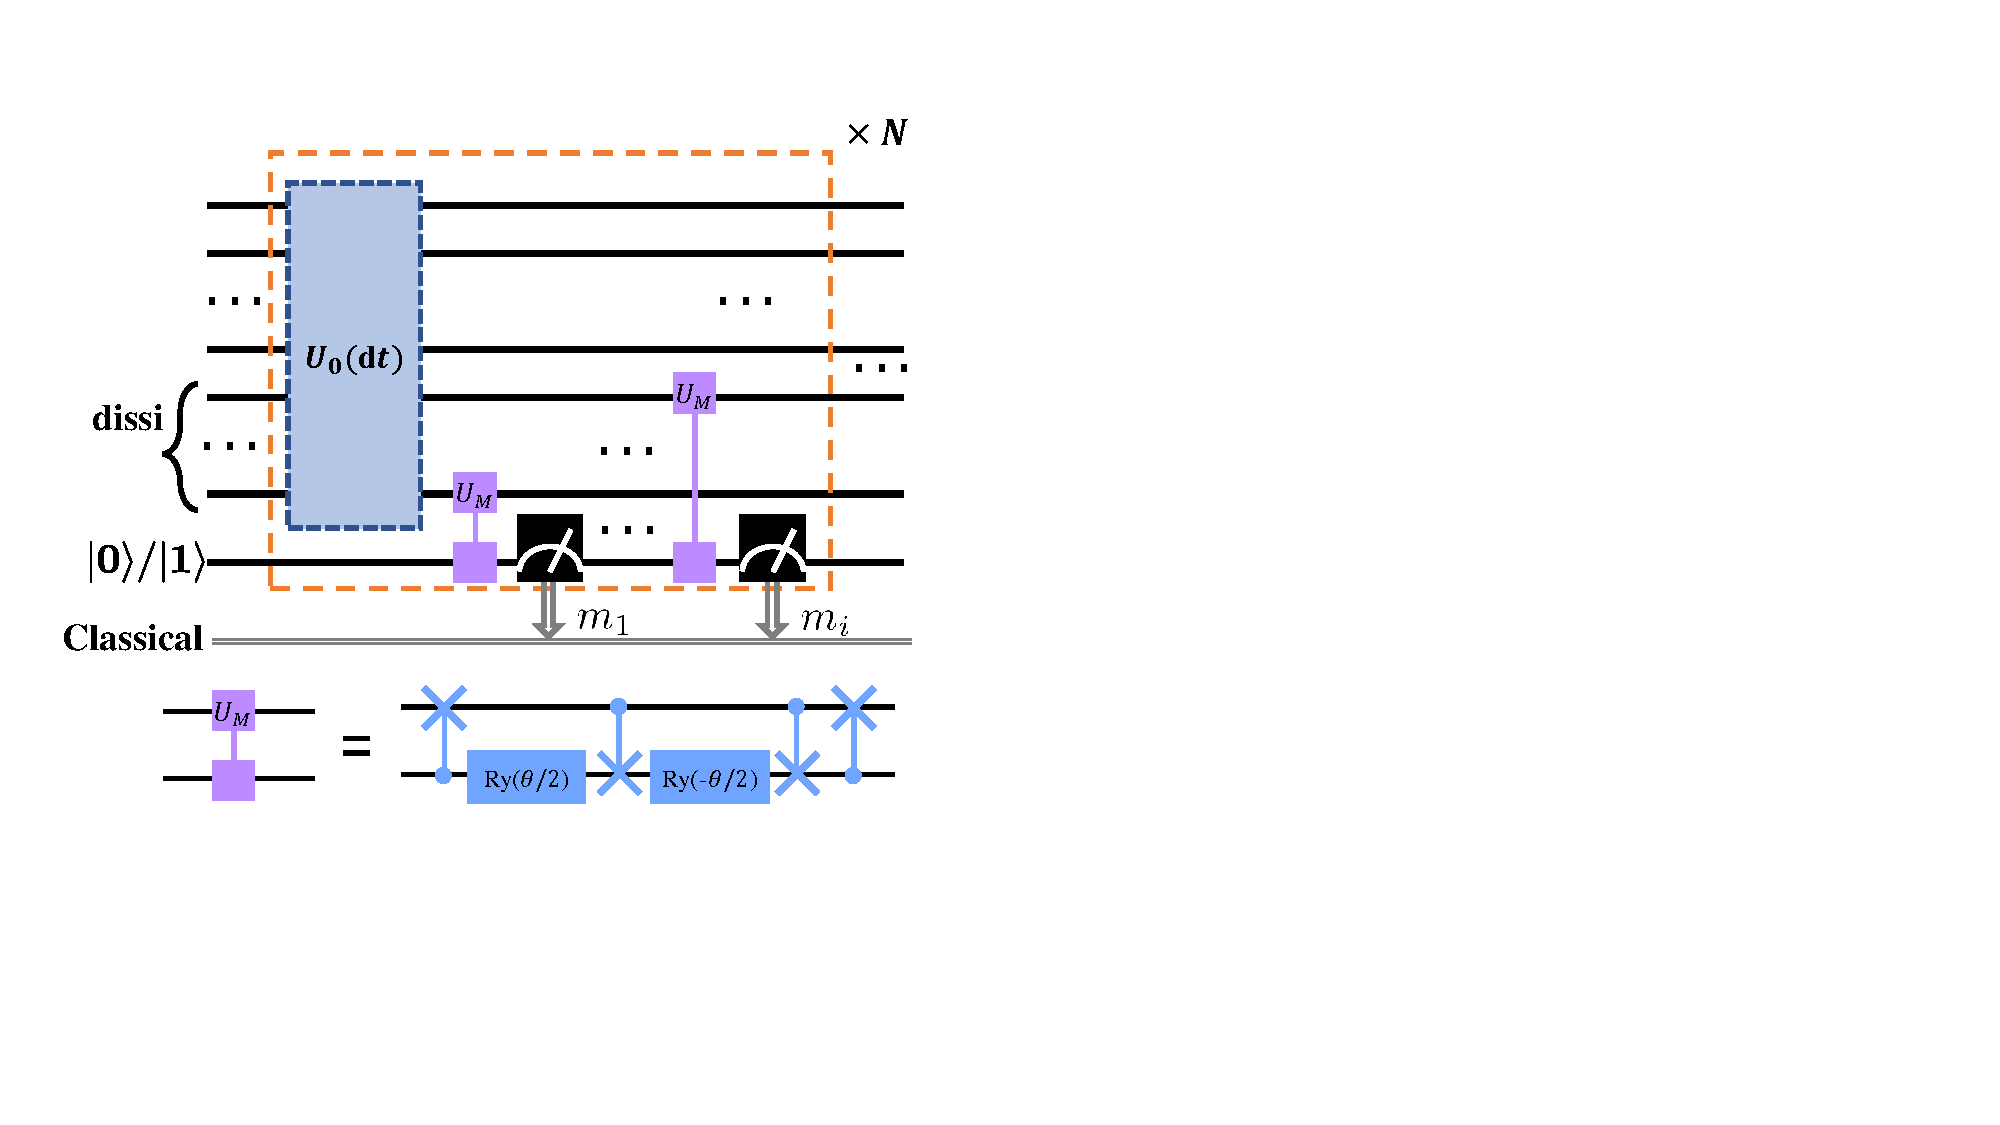
\includegraphics[width=1.\linewidth]{Picture/Circuit_Experiment.pdf}
	% 	\caption{在Qiskit中实现增益/耗散非厄米多体哈密顿量的受控量子线路的示意图，每一个比特代表晶格的一个格点，$\ket{0}/\ket{1}$表示辅助量子比特，用来实现作用在耗散格点(标记为'dissi')的非厄米演化。厄米部分的时间演化$U_0(\mathrm{d}t)$通过量子门实现。作用$N$层演化之后得到$N\mathrm{d}t$时间的演化。作用在耗散格点和辅助比特的量子门可以通过CNOT门和单比特门实现。}
	% 	\label{fig:07}
	% \end{figure}
	% hexagon, thin diamond, cross triangle
	\begin{figure*}[htbp]
		\begin{minipage}[b]{0.61\textwidth}
			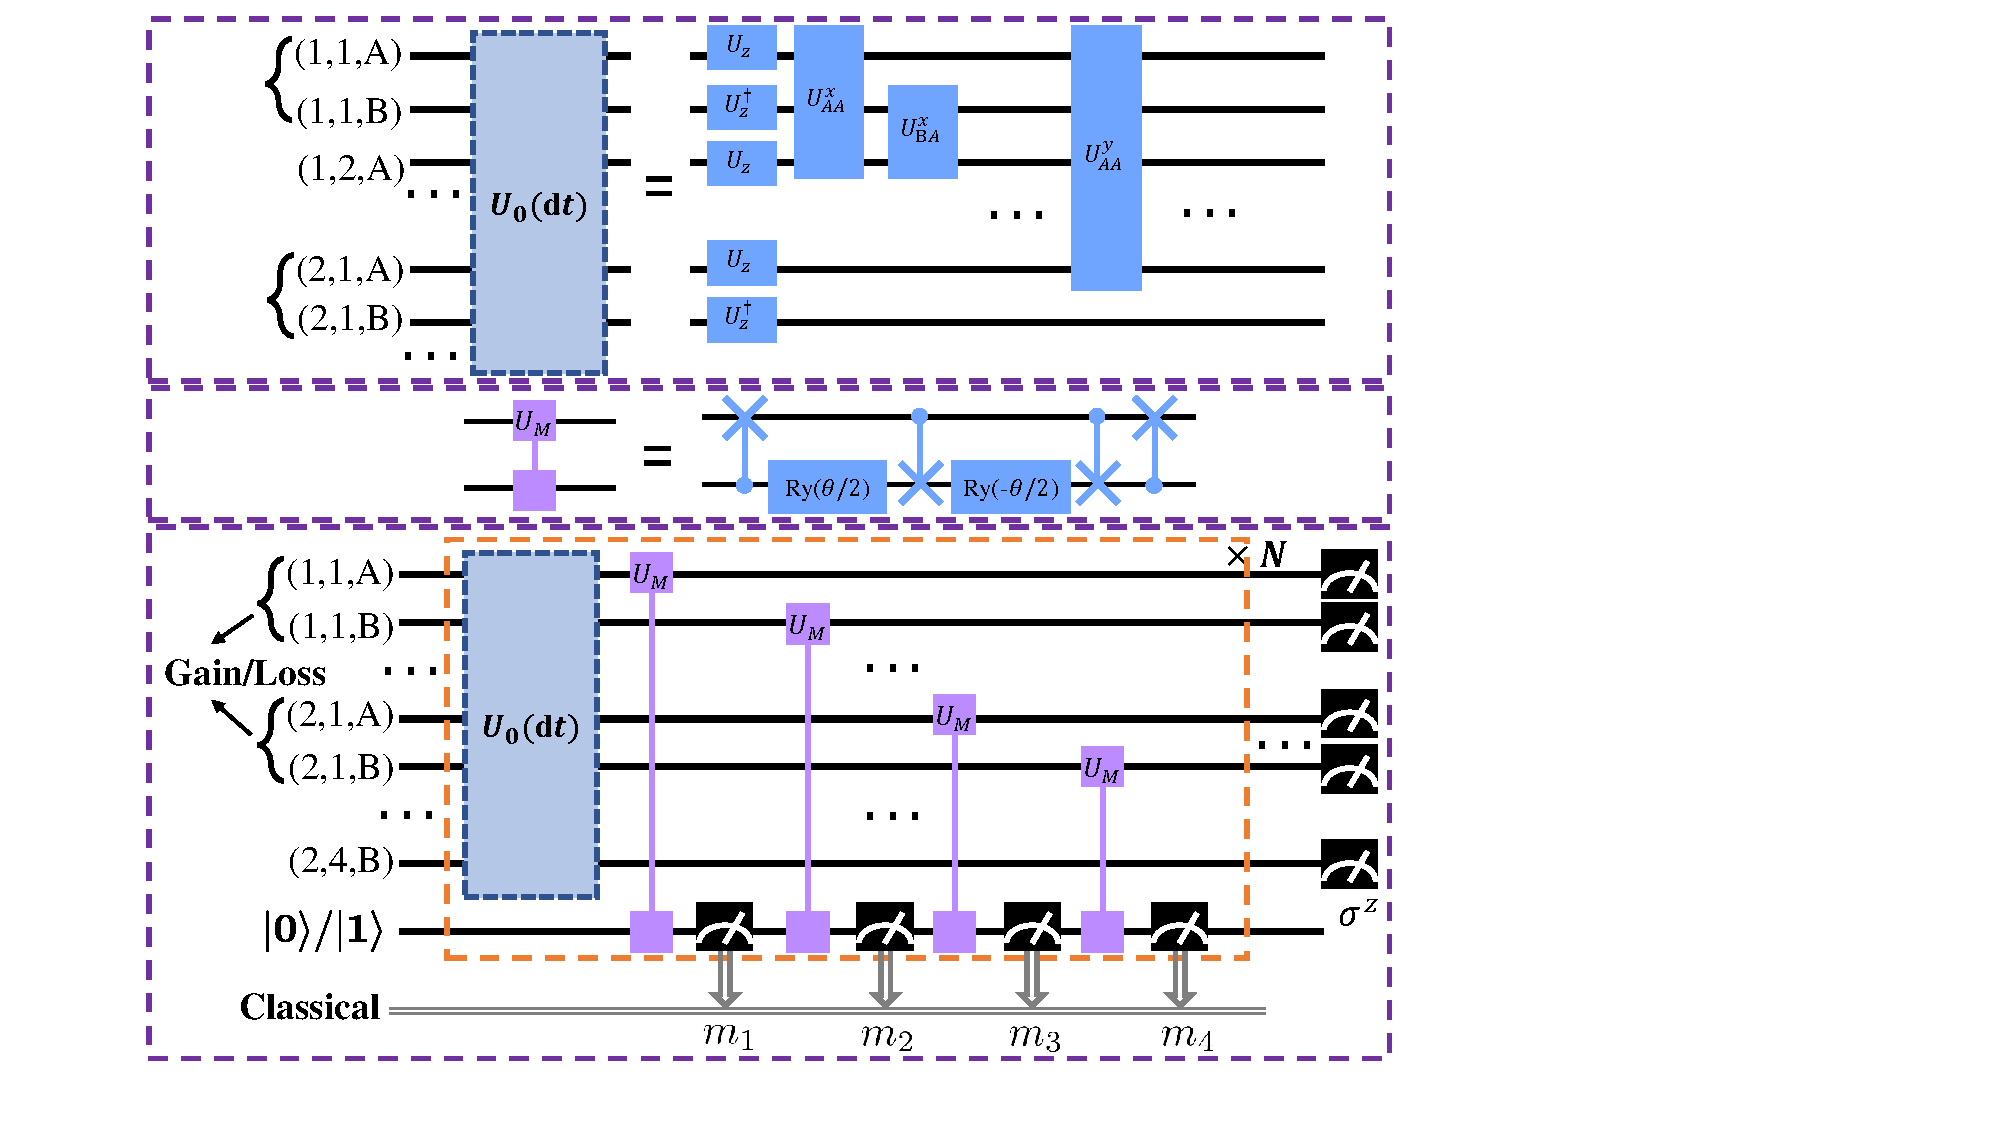
\includegraphics[width=\textwidth]{Picture/RunCircuit.pdf}
			% \caption{图片3说明}
			% \label{fig:img3}
		\end{minipage}
		\hfill
		\begin{minipage}[b]{0.37\textwidth}
			% 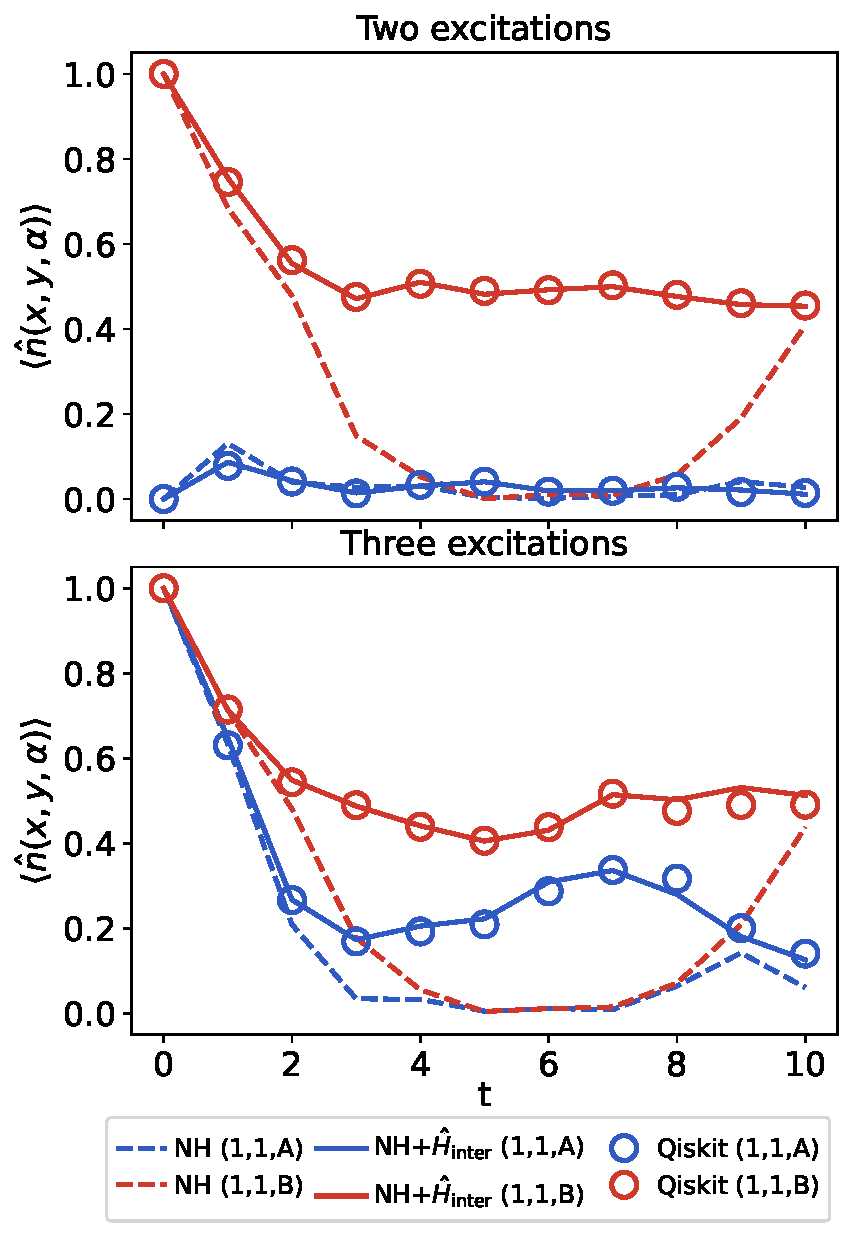
\includegraphics[width=\textwidth]{Picture/MQC_Comp.pdf}
			\begin{overpic}[width=\linewidth]{Picture/MQC_Comp.pdf}
				% \put(-90,198){(a)}
				% \put(7,54){(c)}
				\put(-118,97){(a)}
				\put(1,97){(b)}
				% \put(49,54){(d)}
			\end{overpic}
			% \caption{图片4说明}
			% \label{fig:img4}
		\end{minipage}
		\caption{%(a) 在Qiskit中实现增益/耗散非厄米多体哈密顿量的实际受控量子线路图，每一个比特代表晶格的一个格点，$\ket{0}/\ket{1}$表示辅助量子比特，用来实现作用在耗散格点(标记为'dissi')的非厄米演化。厄米部分的时间演化$U_0(\mathrm{d}t)$通过量子门实现。广义测量$M_i$通过作用在耗散格点和辅助比特的两比特门和随后作用在辅助比特的单比特$\hat{\sigma}_z$实现。作用在耗散格点和辅助比特的量子门可以通过CNOT门和单比特门$R_y(\theta/2)$实现。受控量子线路参数为$\mathrm{d}t=0.2$,$N=50$。
		%(b) 从初始在元胞$(1,1)$和$(1,2)$的$B$子格点各有一个粒子在量子线路下演化，在不同时间$t$测量不同格点的平均粒子数。分别是通过(a)的量子线路和精确计算得到的。系统尺寸为$L_x=2,L_y=4$，相互作用强度为$U_{\text{inter}}=1.0$，非厄米参数为$\gamma=0.2$。受控量子线路参数为$\mathrm{d}t=0.2$,$N=50$。
		%双激发的时，两个粒子分别从$(1,1,B)$和$(2,1,B)$开始演化。三激发时，三个粒子分别从$(1,1,B)$，$(2,1,B)$和$(1,1,A)$开始演化。
		(a) The MQCs implemented in Qiskit for realizing the gain/loss non-Hermitian many-body Hamiltonians. Each qubit represents a lattice site, where the states $\ket{0}/\ket{1}$ correspond to auxiliary qubits used to implement the non-Hermitian evolution on gain/loss lattice sites (marked as 'gain/loss'). The time evolution of the Hermitian part $U_0(\mathrm{d}t)$ is realized with quantum gates. 
		Generalized measurements $M_i$ are implemented by applying two-qubit gates $U_{\text{M}}$ between gain/loss lattice sites and the auxiliary qubit, followed by a single-qubit $\hat{\sigma}_z$ measurements on the auxiliary qubit.
		The two-qubit gates $U_{\text{M}}$ can be realized with CNOT gates and single-qubit $R_y(\theta/2)$ gates. The parameters of the MQCs are $\mathrm{d}t=0.2$,$N=50$.
		(b) Evolution of the average particle number at different lattice sites over time $t$ under the MQCs in (a). 
		%The evolution starts from the initial state where two particles are located on the $B$ sublattice of unit cell $(1,1)$ and $(1,2)$. 
		For two excitations, the initial state consists of two particles located at $(1,1,B)$ and $(2,1,B)$. For three excitations, the initial state consists of three particles located at $(x,y,\alpha)=(1,1,B), (2,1,B), (1,1,A)$.
		The results are obtained through both the MQCs described in (a) and exact calculations. The system size is $L_x=2,L_y=4$. The interaction strength is $U_{\text{inter}}=1.0$ and the non-Hermitian parameter is $\gamma=0.2$. The parameters of the MQCs are $\mathrm{d}t=0.2$,$N=50$.
		}
		\label{fig:04}
	\end{figure*}
	% 应该可以通过一个辅助比特实现，采用Qiskit的线路。然后给出参数。
	The MQCs for simulating a non-Hermitian Hamiltonian we adapted in Qiskit is as Fig.~\ref{fig:04} (a). The time evolution of the Hermitian part, including $\hat{H}_{\text{QWZ}}$ and many-body interaction term $\hat{H}_{\text{inter}}$, is implemented through quantum gates. 
	%To simulate the dynamics in quantum circuits, we first apply the Jordan-Wigner transition to the Hamiltonian. 
	Qubit state $\ket{1}$ represents the occupation of the site and qubit state $\ket{0}$ represents the unoccupation of the site. 
	% Throughout this work, the $A$ and $B$ sublattice site of the unit cell $(x, y)$ are arranged according to $2(y+L_y x)+1$ and $2(y+L_y x)+2$. 
	%Throughout this work, we employ the following sublattice indexing convention: for each unit cell $(x,y)$, the $A$ and $B$ sublattice sites are respectively encoded as $2(y+L_y x)+1$ and $2(y+L_y x)+2$.
	The anticommutation relation of fermionic operators introduces a phase factor -1 when two fermions are exchanged. To maintain this property in our qubit representation, we implement the Jordan-Wigner transformation on the Hamiltonian.
	%the indices $2(y+L_y x)+1$ and $2(y+L_y x)+2$ of basis $\ket{11000\cdots}$ denote the $A$ and $B$ sublattice site of the unit cell $(x, y)$, respectively. 
	Under the Jordan-Wigner transformation, each term of hopping term can be implemented though multi-qubit gates, and each term of interaction Hamiltonian $\hat{H}_{\text{inter}}$ can be implemented though two-qubit gates, as shown in Fig.~\ref{fig:04}(a). 
	% 厄米哈密顿量的时间演化可以通过将系统的演化分解为量子门来实现，如跃迁项的时间演化$e^{-\mathrm{i} \frac{1}{2} (\hat{c}_{1,2,A}^{\dagger} \hat{c}_{1,1,A} +h.c.)\mathrm{d} t}$经过Jordan-Wigner变换之后为$e^{-\mathrm{i} \frac{1}{2} (\hat{\sigma}_{1,2,A}^{+\dagger} \hat{\sigma}^z_{1,1,B}\hat{\sigma}_{1,1,A}^{-} +h.c.)\mathrm{d} t}$，这对应一个三比特门，在Fig.~\ref{fig:04}中用$U_{AA}^x$标记。通过同样的方式可以将厄米哈密顿量的其它项通过量子线路实现，如Fig.~\ref{fig:04}中$U_{BA}^x$表示格点$(1,1,B)$和格点$(1,2,A)$跃迁项的时间演化；$U_{AA}^y$表示格点$(1,1,A)$和格点$(2,1,A)$跃迁项的时间演化。而相互作用项由于是粒子数算符，因此全部可以通过两比特门实现。

	The time evolution of the Hermitian Hamiltonian can be implemented by decomposing the system's evolution into quantum gates. The time evolution of the hopping term $e^{-\mathrm{i} (\hat{c}_{1,2,A}^{\dagger} \hat{c}_{1,1,A} + \text{h.c.})\mathrm{d} t/2}$ can be transformed into a three-qubit gate via the Jordan-Wigner transformation, represented as $e^{-\mathrm{i} (\hat{\sigma}_{1,2,A}^{\dagger} \hat{\sigma}^z_{1,1,B}\hat{\sigma}_{1,1,A}^{-} + \text{h.c.})\mathrm{d} t/2}$. This three-qubit gate is marked as $U_{AA}^x$ in Fig.\ref{fig:04}. Similarly, the time evolution of other terms in the Hermitian Hamiltonian can be implemented via quantum circuits. For example, $U_{BA}^x$ in Fig.\ref{fig:04} corresponds to the time evolution of the hopping term between sites $(1,1,B)$ and $(1,2,A)$, while $U_{AA}^y$ represents the time evolution of the hopping term between sites $(1,1,A)$ and $(2,1,A)$. The interaction terms can be realized using two-qubit gates.

	The time evolution of the non-Hermitian part is implemented through the measurements on one ancillary qubit. 
	All generalized measurements in our scheme can be implemented through only one ancilla. To realize the gain (loss) non-Hermitian Hamiltonian dynamics, we initialize the ancillary qubit to state $\ket{1}$ ($\ket{0}$). And we apply the two-qubit unitary gates $U_M$ to the dissipative sites and the ancillary qubit, as shown in Fig.~\ref{fig:04}. The unitary gates $U_M$ can be realized through CNOT gates and $R_y(\theta) = e^{-\mathrm{i} \hat{\sigma}_y \theta}$ ($\theta = \arccos(e^{-\gamma \mathrm{d}t})$) gates, as shown in Fig.~\ref{fig:04}(a). 
	After applying the unitary gates, we measure the ancillary qubit and store the measurement outcomes in classical registers. 
	We postselect quantum trajectories when the results on classical register are $\ket{1}$($\ket{0}$) to realize the evolution of gain(loss) non-Hermitian Hamiltonians. By repeating this circuit $N$ times, we effectively simulate non-Hermitian dynamics of time $N\mathrm{d}t$.
	%我们选择所有经典寄存器结果都是$\ket{1}$($\ket{0}$)的量子轨迹，可以实现增益(耗散)非厄米哈密顿量的演化。

	The comparisons between the results of the MQC and exact time-evolution are given in Fig.~\ref{fig:04} (b). 
	%我们考虑一个$L_x=2,L_y=4$的二维晶格，耗散作用于$y=1$的边界上，相互作用部分为$U_{\text{inter}}=1.0$的$\hat{H}_{\text{inter}}$。
	We consider a two-dimensional lattice with dimension $L_x=2$ and $L_y=4$, and the gain is implemented on the boundary at $y=1$. The interaction strength of $\hat{H}_{\text{inter}}$ is $U_{\text{inter}}=1.0$.
	% 我们激发两个粒子，这两个粒子初始位于格点$(1,1,B)$和$(2,1,B)$。然后，我们分别数值计算了在非厄米哈密顿量（dashed lines）和非厄米多体哈密顿量(solid line)下的演化。同时我们还利用Fig.~\ref{fig:04} (a)的量子线路模拟了非厄米多体哈密顿量的演化(hollow circles)，在随后的时间对各个格点测量$\langle \hat{n}_{x,y,\alpha}\rangle$，相应的结果在Fig.~\ref{fig:04} (b)中。蓝色表示在格点$(1,1,A)$的粒子数平均值；红色表示在格点$(1,1,B)$的粒子数平均值。
	There are initially two fermions at lattice sites $(1,1,B)$ and $(2,1,B)$. Through numerical calculations, we investigate the system's evolution under both the non-Hermitian Hamiltonian (dashed lines) and the non-Hermitian many-body Hamiltonian (solid lines). Additionally, we simulate the evolution under the non-Hermitian many-body Hamiltonian with the quantum circuit shown in Fig.~\ref{fig:04} (a) (hollow circles) and measure the average article number $\langle \hat{n}(x,y,\alpha)\rangle$ at subsequent time. The results are presented in Fig.~\ref{fig:04} (b), where the blue curves and points represent the average particle number at site $(1,1,A)$, and the red curves and points represent the average particle number at site $(1,1,B)$.

	% Fig.~\ref{fig:04}中的结果显示出通过Qiskit模拟的结果与精确计算的结果一致。它们之间的吻合表明我们的方案的MQC确实能够仅通过一个辅助比特对增益非厄米多体哈密顿量进行模拟。非厄米哈密顿量与非厄米多体哈密顿量的结果在时间$t=2$时显示出二者的区别。在非厄米哈密顿量演化下，位于格点$(1,1,B)$的粒子会完全跃迁到其它格点上，然后又会跃迁回来。而在非厄米多体哈密顿量演化下，从该初态演化的粒子会很快演化到稳态，然后在该态上的粒子数不再变化，这一粒子数巨大的区别可以被实验探测到，进而展现多体相互作用对非厄米演化的作用。
	The results in Fig.~\ref{fig:04} (b) demonstrate that the simulations of the non-Hermitian many-body Hamiltonian using Qiskit are consistent with the results of exact calculation. This consistency validates that our scheme based on MQC can accurately simulate the gain/loss non-Hermitian many-body Hamiltonian with just one auxiliary qubit. 
	At time $t=4$, the results under the non-Hermitian Hamiltonian and the non-Hermitian many-body Hamiltonian show significant differences. 
	For the evolution of the non-Hermitian Hamiltonian, we observe complete population transfer from site $(1,1,B)$ followed by revival.
	% Specifically, under non-Hermitian Hamiltonian, the particle at site $(1,1,B)$ completely jumps to other sites and then returns. 
	In contrast, the non-Hermitian many-body Hamiltonian drives the system toward a steady state with frozen particle number distributions.
	% In contrast, under non-Hermitian many-body Hamiltonian, the system quickly evolves into a steady state, where the particle number at each site remains constant. 
	These measurable occupation patterns provide direct experimental signatures of how many-body interactions fundamentally alter non-Hermitian quantum dynamics.
	% This significant difference in particle number can be experimentally measured, thereby revealing the impact of many-body interactions on the non-Hermitian evolution.
	
	% 我们同时研究了从三激发量子态出发的演化，这三个粒子初始处于格点$(1,1,A),(1,1,B)$和$(2,1,B)$。在非厄米多体哈密顿量下，位于格点$(1,1,B)$的粒子数会衰减，最后也会达到稳态，但是位于格点$(1,1,A)$的粒子会跃迁到其它格点，这一点与非厄米哈密顿量的行为完全不同。所以在不同的激发子空间中，都能观察到系统在非厄米多体哈密顿量的演化下能够更快演化到稳态(Fig.~\ref{fig:04} (b)的solid lines)，这与不存在多体相互作用的非厄米哈密顿量存在显著区别(Fig.~\ref{fig:04} (b)的dashed lines)。从四激发量子态出发，精确模拟的结果与通过Qiskit模拟的结果在Appendix.~\ref{sec:appendF_4Body_Evolve}进行了详细的讨论。
	In addition, we investigate the evolution of three excitations, where the three excitations are initially located at sites $(1,1,A), (1,1,B)$, and $(2,1,B)$. 
	Under the evolution of the non-Hermitian many-body Hamiltonian, the particle number at site $(1,1,B)$ quickly decays to a steady value.
	%, while the particle at site $(1,1,A)$ jumps to other sites. 
	This contrasts sharply with the non-interacting non-Hermitian case (as shown by the dashed line in Fig.\ref{fig:04}(b)), where such steady particle number is absent.
	%This behavior is different from that under the evolution of non-Hermitian Hamiltonian. 
	Through the numerical simulation across different fermionic excitations, we show that the system evolves more rapidly into a steady state under a non-Hermitian many-body Hamiltonian (as shown by the solid lines in Fig.\ref{fig:04}(b)). 
	%This is different from the results under the evolution of non-Hermitian Hamiltonian without many-body interactions (as shown by the dashed lines in Fig.\ref{fig:04}(b)). 
	% A detailed discussion about the evolution of four excitations based on the exact calculations and quantum circuit simulations is provided in Appendix~\ref{sec:appendF_4Body_Evolve}. %这儿强调一致性，但是又没有提激发数下的hybrid态，还加嘛？可以把附录G只表示成图6b的形式。
	%更多粒子的在MQC中的演化在Appendix.~\ref{sec:4Body_Evolve}中进行了详细阐述。
	% 在其它格点的粒子数平均值的结果在Appendix.~\ref{sec:4Body_Evolve}中。

	% \begin{figure}[h]
	% 	\centering
	% 	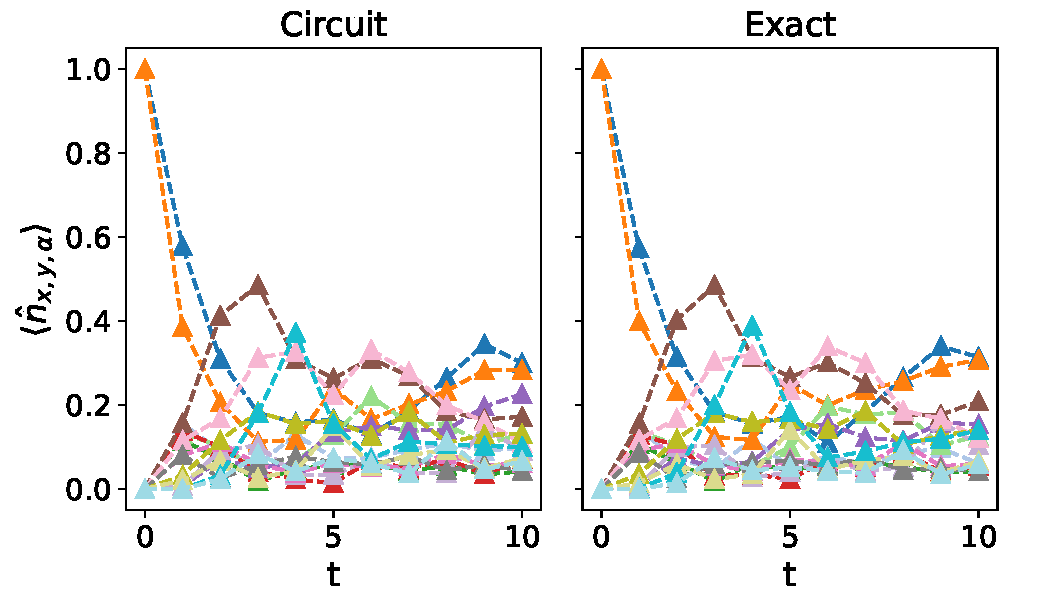
\includegraphics[width=1.\linewidth]{Picture/CircuitEvolve_ManyBody.pdf}
	% 	\caption{从初始在元胞$(1,1)$和$(1,2)$的$A$子格点各有一个粒子开始演化，在不同时间$t$不同格点的平均粒子数。分别是通过Fig.~\ref{fig:07}的量子线路和精确计算得到的。系统尺寸为$L_x=2,L_y=4$，相互作用强度为$U_{\text{inter}}=1.0$，非厄米参数为$\gamma=0.2$。受控量子线路参数为$\mathrm{d}t=0.2$,$N=50$}
	% 	\label{fig:08}
	% \end{figure}

	The approach proposed here can be further experimentally demonstrated using superconducting qubits, trapped ions, or photonic quantum processors by engineering non-reciprocal couplings and controlled dissipation. State-of-the-art noisy intermediate-scale quantum (NISQ) devices, featuring hundreds of qubits, provide a viable platform for implementation. For instance, superconducting qubit array with tunable couplings and high coherence \cite{guo2021observation, preskill2018quantum, wu2021strong} or large-scale photonic quantum simulators with programmable linear optical networks \cite{zhong2020quantum, madsen2022quantum, zhu2024dynamically} could be employed to realize the MQC implementation. Linear qubit gates can be readily implemented using parametric couplers for superconducting qubits or directional couplers and phase modulators for photonic systems \cite{zhu2024large}. A key challenge in realizing many-body non-Hermitian dynamics in MQCs is the implementation of controlled gain or loss. Fortunately, a single ancillary qubit suffices to simulate all necessary generalized measurements. In photonic systems, engineered loss can be introduced via additional modes or waveguide couplings~\cite{hoch2025quantum, carolan2020variational}, while superconducting platforms can leverage mid-circuit measurements to emulate non-Hermiticity~\cite{shen2024enhanced,shen2025observation}. After preparing the Hamiltonian evolution on quantum hardware, exponential localization at boundaries can be observed through qubit measurements or photon detection.  In future work, our proposal can be directly implemented in state-of-the-art superconducting and photonic quantum platforms. Thus, this work paves the way for exploring non-Hermitian topology in NISQ devices.

	\section{Conclusion}
	Applying gain/loss at the boundaries of a system gives rise to single-particle topological phenomena, such as the chiral skin effect. Upon introducing many-body interactions, we uncover hybrid chiral skin correlated states, which are distinct from multi-particle chiral skin modes. This distinction can be revealed through both site-resolved occupation numbers and correlation functions, highlighting the nontrivial interplay between non-Hermitian topology and many-body interaction. 
	To systematically explore non-Hermitian many-body physics, we develop a programmable MQCs framework based on the universality of digital quantum computers. 
	With this MQCs framework, we simulate these hybrid states on Qiskit using only a single ancillary qubit in two-dimensional lattice configurations. 
	Our study of the interplay between non-Hermitian topology and many-body interactions not only establishes a concrete route toward simulating and controlling non-Hermitian many-body phenomena in two-dimensional systems, but also offeres broadly applicable insights for future studies of correlated open quantum matter.

	\section{Methods~\label{sec:method}}
	% \subsection{Implementation the gain/loss Hamiltonian in MQCs}
	% % 不用管那个，因为mqc本身实现非厄米，nc又不是第一篇
	% % 就按照我们自己的来写。最后落脚在chiral skin就行

	% In this part, we show how to realize the time evolution of the gain/loss non-Hermitian Hamiltonian. The non-Hermitian Hamiltonian $\hat{H}_{\text{non}}$ consists of Hermitian part $\hat{H}_0$, such as the Hamiltonian of QWZ model, and non-Hermitian part $\hat{H}_{\text{im}}$.
	% \begin{equation}
	% 	\hat{H}_{\text{non}} = \hat{H}_0 +\hat{H}_{\text{im}}. \label{eq:non-hermitian}
	% \end{equation}
	% The non-Hermitian part $\hat{H}_{\text{im}}$ is the sum of gain/loss energy on each site, which holds imaginary onsite energy, such as $\hat{H}_{\text{im}} = \sum_{i\in \text{dissi}} -\mathrm{i}\tilde{\gamma} \hat{c}_i^{\dagger} \hat{c}_i$ for dissipative energy. 
	% %The time evolution of the Hermitian part. 
	% To realize the time evolution of non-Hermitian Hamiltonian with time \textit{t}, labeled as $U(t) = e^{-\mathrm{i}(\hat{H}_0+\hat{H}_{\text{im}})t}$, we first construct $U(\mathrm{d} t)$ and  
	% % The condition of dt is defined below.
	% $U(t)$ is constructed by repeatedly acting $U(\mathrm{d} t)$.
	% We define $\mathrm{d} t$ as the measurement interval, which is the unitary evolution time between measurements in two layers.
	
	% To realize $U(\mathrm{d} t)$, we first act the time evolution of $\hat{H}_{0}$, labeled  as $U_0(\mathrm{d}t)=e^{-\mathrm{i}\hat{H}_0 \mathrm{d} t}$, and then local generalized measurements on the gain/loss sites, see Fig.~\ref{fig:01}.
	% %In addition, we should emphasize that this projective measurement can be cancelled in each layer and a projective measurement on the ancilla at the end of the whole process is enough.
	% % P0 at the end of the whole process is enough, the provement or statement should be added
	% The generalized measurements are defined as a set of Kraus operators $\{M_{i,\beta},\beta=0,\pm \}$, which are a completely positive trace-preserving map. Without any postselection, the map is defined as
	% $\varepsilon(\rho) = \sum_{\beta} M_{i, \beta} \rho M_{i, \beta}^{\dagger}$, and $\rho$ is density matrix of the fermionic system.
	% The generalized measurements on the ith site are defined as
	% \begin{align}
	% 	&M_{i,\pm} = \sqrt{\frac{1}{2+(e^{\gamma \mathrm{d} t} - e^{-\gamma \mathrm{d} t})^2}} (1 + (e^{\pm \gamma \mathrm{d} t}-1) \hat{c}_i^{\dagger} \hat{c}_i),\\
	% 	&M_{i,0} = \sqrt{\frac{(e^{\gamma \mathrm{d} t} - e^{-\gamma \mathrm{d} t})^2}{2+(e^{\gamma \mathrm{d} t} - e^{-\gamma \mathrm{d} t})^2}} c_i^{\dagger},
	% \end{align}
	% which satisfy the trace-preserving condition $\sum_{\beta} M_{i,\beta}^{\dagger} M_{i,\beta}=\mathrm{I}$. 
	% Note that measurement interval $\mathrm{d}t$ is a parameter in the generalized measurements. 
	% The generalized measurements can also be denoted as 
	% \begin{align}
	% 	&M_{i,\pm} = \sqrt{\frac{1}{2+(e^{\gamma \mathrm{d} t} - e^{-\gamma \mathrm{d} t})^2}} e^{\pm\gamma \hat{c}_i^{\dagger} \hat{c}_i\mathrm{d} t},\\
	% 	&M_{i,0} = \sqrt{\frac{(e^{\gamma \mathrm{d} t} - e^{-\gamma \mathrm{d} t})^2}{2+(e^{\gamma \mathrm{d} t} - e^{-\gamma \mathrm{d} t})^2}} c_i^{\dagger}.
	% \end{align}	
	% Although not all operations can be implemented, the measurements above can be realized through projection measurements in an enlarged Hilbert space, as guaranteed by the Naimark's theorem~\cite{coecke2008povms,nielsen2001quantum}. As a result, our scheme can be implemented with current experimental techniques through the introduction of auxiliary qubits.
	% The dissipative non-Hermitian Hamiltonian with onsite loss $-\mathrm{i}\gamma$ can be realized through postselecting $M_{i,-}$, while the non-Hermitian Hamiltonian with onsite gain $\mathrm{i}\gamma$ can be realized through postselecting $M_{i,+}$.
	% % under what condition, it is a projective measurement!(no) Explain our measurement. 
	
	% Our measurement scheme postselects the outcome of $M_{i,-}$ for dissipative non-Hermitian, which maps the state $\vert \psi \rangle$ to $M_{i,-} \vert \psi \rangle/\Vert M_{i,-} \vert \psi \rangle \Vert$ with a probability of $\Vert M_{i,-} \vert \psi \rangle \Vert^2$. 
	% %If the Hermitian part $\hat{H}_0$ and the non-Hermitian part $\hat{H}_{\text{im}}$ are not commutative, 
	% The parameter of measurements should satisfy $\gamma \mathrm{d} t \ll 1$. To postselect the $M_{i,-}$ over n measurements, we need roughly to perform  $2^n$ experiments. 
	% % how to realize the POVM, add some citations.
	% %Unitary evolution of $\hat{H}_0$ followed by postselective measurements on all dissipative sites is described as $E=(\prod_{i\in \text{dissi}} M_{i,-}) U_{0}(\mathrm{d} t),U_{0}(\mathrm{d}t)=e^{-\mathrm{i}\hat{H}_0 \mathrm{d}t}$. 
	% The whole evolution process is to first perform the unitary evolution of $\hat{H}_0$ on all sites and then the generalized measurements on all dissipative sites. It is described as $E=(\prod_{i\in \text{dissi}} M_{i,-}) U_{0}(\mathrm{d} t),U_{0}(\mathrm{d}t)=e^{-\mathrm{i}\hat{H}_0 \mathrm{d}t}$.
	% Instead of performing all measurements on gain/loss sites, our scheme performs the measurement on each gain/loss site with a classical probability $p\in(0,1]$.
	% %, see Fig.~\ref{fig:monitoredquantumcircuit}(a). 
	% Then we obtain a probabilistic quantum circuit operator, and the process of performing it on an initial state $\vert \psi \rangle$ is described by
	% \begin{equation}
	% 	\frac{E(p,r) \vert \psi \rangle}{\Vert E(p,r) \vert \psi \rangle \Vert} = \frac{(\prod_j M_{j,-}^{r_j}) \cdot U_0(\mathrm{d}t)}{\Vert (\prod_j M_{j,-}^{r_j}) \cdot U_0(\mathrm{d}t) \vert \psi \rangle \Vert} \vert \psi \rangle,
	% \end{equation}
	% where $U_0(\mathrm{d} t) = e^{-\mathrm{i}\hat{H}_0 \mathrm{d} t}$ and $r_j$ = 0 or 1 with a probability of $1-p$ and $p$, respectively. So $N$-layer MQC with a probability of $p$ is defined as
	% \begin{equation}
	% 	E_N(p,\{r\}) = E(p, r_N) \circ E(p, r_{N-1}) \circ \cdots \circ E(p, r_1).
	% \end{equation}
	% % define effective Hamiltonian
	% The effective Hamiltonian $\hat{H}_{\text{eff}}^{(N)}$ of this $N$-layer MQC is defined as
	% \begin{equation}
	% 	e^{-\mathrm{i}\hat{H}_{\text{eff}}^{(N)} N \mathrm{d} t} = E_N(p,\{r\}). \label{eq:H_scheme1}
	% \end{equation}
	\iffalse
	We define the effective Hamiltonian of a finite \textit{N}-layer quantum circuit as 
	\begin{align}
		\hat{H}^{(N)}_{\text{eff}} (p,\mathrm{d}t, \{s\}) &= \frac{i}{N\mathrm{d}t} \log{E_N(p, \{r\})} \notag\\
		&= \frac{i}{N\mathrm{d}t} \sum_{i=1}^N \log{E(p,r_i)}. \label{eq:EffectiveH}
	\end{align}\
	\fi
	
	%Take Fig.~\ref{fig:monitoredquantumcircuit}(c) as an example, the non-Hermitian Hamiltonian is defined on a square lattice, where the red points indicate the unit cells and the red points in the blue rectangle indicate the gain (loss) unit cells with $\mathrm{i}\gamma \sigma_0$ ($-\mathrm{i}\gamma \sigma_0$ ) imaginary onsite energy, where $\sigma_0$ is the identity matrix. The first scheme to realize this non-Hermitian Hamiltonian is to apply unitary evolution $U_0(\mathrm{d}t)$ of the Hermitian part. And then each generalized measurement in the blue rectangle is applied with probability $p$. The above sequence is one layer of the quantum circuit, and $N$-layer quantum circuit can realize $N\mathrm{d}t$ time evolution of the non-Hermitian Hamiltonian, as depicted in Fig.~\ref{fig:monitoredquantumcircuit}(a). 

	% \subsection{The relationship between measurement-induced topology and non-Hermitian topology}
	\subsection{The construction of non-Hermitian many-body Hamiltonians based on MQCs~\label{sec:scheme_method}}

	We propose a general scheme to realize the evolution of gain/loss non-Hermitian Hamiltonian in the MQCs.
	The general form of such Hamiltonians contains both Hermitian and non-Hermitian components:
	\begin{equation}
		\hat{H} = \hat{H}_0 +\hat{H}_{\text{im}}. \label{eq:non-hermitian}
	\end{equation}
	% The Hermitian part $\hat{H}_0$ is the sum of onsite energy $\hat{c}_i^{\dagger}\hat{c}_i$, hopping term $\hat{c}_i^{\dagger}\hat{c}_j$, and the interaction term $\hat{n}_i\hat{n}_j$. 
	The non-Hermitian part $\hat{H}_{\text{im}}$ is the sum of gain/loss energy on each site, which holds imaginary onsite energy, such as $\hat{H}_{\text{im}} = \sum_{i\in \text{dissi}} \mathrm{i}\tilde{\gamma} \hat{c}_i^{\dagger} \hat{c}_i$ for gain/loss energy. 
	% 上面这段描述多余吗？
	After Jordan-Wigner transformation, the Hamiltonian of fermion system can be implemented through the MQCs, where each lattice site is encoded in a qubit. 
	%The details of Jordan-Wigner transformation can be found in Methods.  
	Throughout this work, the qubit state $\ket{0}$ ($\ket{1}$) indicates the absence (presence) of a fermion at the lattice site.
	% The effective dynamics of this MQCs and the realization of the generalized measurements $M_i$ are presented in Sec.\ref{sec:method}.
	% 测量什么得到什么量。

	The digital quantum computer can be used to simulate the fermionic system. 
	%Qubit state $\ket{1}$ indicates there is a fermion at the site, and qubit state $\ket{0}$ indicates that there is no fermion at the site. 
	%但是交换不同格点的费米子会出现一个负号，但是量子比特没有这个性质。
	A negative sign will appear when exchanging the fermion at different sites, but qubits do not have this property. 
	% 为了满足费米子算符的对易关系，我们引入一个链算符
	To preserve the fermionic commutation relations, we introduce a string operator defined as
	\begin{equation}
		P_i = \otimes_{j=1}^i\hat{\sigma}^z_j.
	\end{equation}
	%基于该链算符，采用上升算符$\sigma^+=(\sigma^x+\mathrm{i}\sigma^y)/2$和下降算符$\sigma^-=(\sigma^x-\mathrm{i}\sigma^y)/2$表示费米子产生湮灭算符为：
	Using this string operator $P_i$, the fermionic creation and annihilation operators can be expressed in terms of the raising operator $\hat{\sigma}^+=(\hat{\sigma}^x+\mathrm{i}\hat{\sigma}^y)/2$ and the lowering operator $\hat{\sigma}^-=(\hat{\sigma}^x-\mathrm{i}\hat{\sigma}^y)/2$ as follows:
	\begin{equation}
		\begin{split}
			\hat{c}_i = P_i \otimes \hat{\sigma}^{-}\otimes (\otimes_{j=i+1}\hat{\sigma}^0_j)\\
			\hat{c}_i^{\dagger} = P_i \otimes \hat{\sigma}^{+}\otimes (\otimes_{j=i+1}\hat{\sigma}^0_j),
		\end{split}
	\end{equation}
	where $\hat{\sigma}^{x,y,z}$ represent the Pauli matrices and $\hat{\sigma}^0$ represents $2\times 2$ identity matrix. 
	% This transformation is called Jordan-Wigner transformation. 
	
	In general, the underlying interesting phenomena are uncovered through the evolution dynamics in the MQCs. The evolution of non-Hermitian Hamiltonian $U(t) = e^{-\mathrm{i}(\hat{H}_0 + \hat{H}_{\text{im}})t}$ is realized by alternately implementing $\mathrm{d} t$ time evolution of the Hermitian part $U_0(\mathrm{d}t)=e^{-\mathrm{i}\hat{H}_0 t}$ and $\mathrm{d} t$ time evolution of non-Hermitian part. 
	% The effect of $U_0(\mathrm{d}t)$ on the input qubit is shown in the middle of Fig.~\ref{fig:01}(a).
	The evolution of the Hermitian part $\hat{H}_0$ is decomposed via Trotter expansion, and each of them is a multi-qubit gate. 
	% The evolution of the Hermitian part can be realized through quantum gates. 
	% The evolution can be expanded through Trotter expansion, and the evolution of each hopping term including many-body interaction is a multi-qubit quantum gate. 
	The time evolution of non-Hermitian part $\hat{H}_{\text{im}}$ is implemented through generalized measurements $M_i$.
	%, as shown in Sec.\ref{sec:method}. 
	Here, the generalized measurements are defined as a set of Kraus operators $\{M_{i,\beta},\beta=0,\pm \}$, which are a completely positive trace-preserving map. Without any postselection, the map is defined as
	$\varepsilon(\rho) = \sum_{\beta} M_{i, \beta} \rho M_{i, \beta}^{\dagger}$, and $\rho$ is the density matrix of the fermionic system.
	The generalized measurements on the ith site are defined as
	\begin{align}
		&M_{i,\pm} = \sqrt{\frac{1}{2+(e^{\gamma \mathrm{d} t} - e^{-\gamma \mathrm{d} t})^2}} (1 + (e^{\pm \gamma \mathrm{d} t}-1) \hat{c}_i^{\dagger} \hat{c}_i),\\
		&M_{i,0} = \sqrt{\frac{(e^{\gamma \mathrm{d} t} - e^{-\gamma \mathrm{d} t})^2}{2+(e^{\gamma \mathrm{d} t} - e^{-\gamma \mathrm{d} t})^2}} c_i^{\dagger},
	\end{align}
	which satisfy the trace-preserving condition $\sum_{\beta} M_{i,\beta}^{\dagger} M_{i,\beta}=\mathrm{I}$. 
	Note that measurement interval $\mathrm{d}t$ is a parameter in the generalized measurements. 
	% The generalized measurements can also be denoted as 
	% \begin{align}
	% 	&M_{i,\pm} = \sqrt{\frac{1}{2+(e^{\gamma \mathrm{d} t} - e^{-\gamma \mathrm{d} t})^2}} e^{\pm\gamma \hat{c}_i^{\dagger} \hat{c}_i\mathrm{d} t},\\
	% 	&M_{i,0} = \sqrt{\frac{(e^{\gamma \mathrm{d} t} - e^{-\gamma \mathrm{d} t})^2}{2+(e^{\gamma \mathrm{d} t} - e^{-\gamma \mathrm{d} t})^2}} c_i^{\dagger}.
	% \end{align}	
	Although not all operations can be implemented, the measurements above can be realized through projection measurements in an enlarged Hilbert space, as guaranteed by Naimark's theorem~\cite{coecke2008povms,nielsen2001quantum}. As a result, our scheme can be implemented with current experimental techniques through the introduction of auxiliary qubits.
	The dissipative non-Hermitian Hamiltonian with onsite loss $-\mathrm{i}\gamma$ can be realized through postselecting $M_{i,-}$, while the non-Hermitian Hamiltonian with onsite gain $\mathrm{i}\gamma$ can be realized through postselecting $M_{i,+}$. 
	% under what condition, it is a projective measurement!(no) Explain our measurement. 
	
	Our measurement scheme postselects the outcome of $M_{i,-}$ for dissipative non-Hermitian, which maps the state $\vert \psi \rangle$ to $M_{i,-} \vert \psi \rangle/\Vert M_{i,-} \vert \psi \rangle \Vert$ with a probability of $\Vert M_{i,-} \vert \psi \rangle \Vert^2$. 
	%If the Hermitian part $\hat{H}_0$ and the non-Hermitian part $\hat{H}_{\text{im}}$ are not commutative, 
	The parameter of measurements should satisfy $\gamma \mathrm{d} t \ll 1$.
	% To postselect the $M_{i,-}$ over n measurements, we need roughly to perform  $2^n$ experiments. 
	% The non-Hermitian term can be realized through the generalized measurements. 
	The realization of generalized measurements $\{M_{i,\beta}, \beta=\pm,0\}$ is difficult. However, measurements $M_{i,+}$ and measurements $M_{i,-}$ can be realized though one ancillary qubit. We first act a two-qubit unitary gate to the qubit and the ancillary qubit, which is
	\begin{equation}
		U_{\text{M}} = \begin{pmatrix}
		  1 & 0 & 0 & 0\\
		  0 & e^{-\gamma \dif t} & \sqrt{1-e^{-2 \gamma \dif t}} & 0\\
		  0 & -\sqrt{1-e^{-2 \gamma \dif t}} & e^{-\gamma \dif t} & 0\\
		  0 & 0 & 0 & 1
		\end{pmatrix}.
	\end{equation}
	If the ancillary qubit is prepared on state $\ket{0}$($\ket{1}$), the measurement $M_{i,-}$($M_{i,+}$) can be realized when the measurement on the ancillary qubit gives $\ket{0}$ ($\ket{1}$) results. 

	To implement the measurements $M_{i,-}$, we initialize the ancillary qubit in the state $\ket{0}$. For an initial state $\alpha \ket{0} + \beta \ket{1}$, the joint state after applying the unitary operation $U_M$ become
	% The state after applying $U_M$ is 
	%Suppose the initial state $\alpha \ket{0} + \beta \ket{1}$, after applying the $U_M$, we get
	\begin{equation}
		(\alpha \ket{0} + \beta e^{-\gamma \mathrm{d}t} \ket{1}) \otimes \ket{0} - \beta \sqrt{1-e^{-2\gamma\mathrm{d}t}} \ket{0} \ket{1}.
	\end{equation}
	Subsequent projection of the ancillary qubit onto $\ket{0}$ yields the unnormalized system state $\alpha \ket{0} + \beta e^{-\gamma \mathrm{d}t} \ket{1}$. 
	Conversely, for the implementation of $M_{i,+}$, the ancilla is initialized to $\ket{1}$. The joint state after applying $U_M$ is
	\begin{equation}
		(\alpha e^{-\gamma \mathrm{d}t} \ket{0} + \beta  \ket{1}) \otimes \ket{1} + \alpha \sqrt{1-e^{-2\gamma\mathrm{d}t}} \ket{1} \ket{0}.
	\end{equation}
	Projective measurement of the ancilla in $\ket{1}$ then collapses the system to $\alpha e^{-\gamma \mathrm{d}t} \ket{0} + \beta  \ket{1}$.
	%After projecting the ancillary qubit to state $\ket{1}$, we get state $\alpha e^{-\gamma \mathrm{d}t} \ket{0} + \beta  \ket{1}$.
	Through the two-qubit gates and the $\hat{\sigma}_z$ measurements on the ancillary qubit, we can realize the time evolution  of non-Hermitian Hamiltonian $e^{-\mathrm{i} (\pm \mathrm{i} \hat{c}_i^{\dagger}\hat{c}_i) \mathrm{d}t}$.
	% The corresponding description in the MQCs is shown as purple squares $U_{M}$ in Fig.~\ref{fig:01}(a).
	% 最后给出后选择概率，说明比较容易实现。可以提一下Zeno效应吗？
	% how to realize the POVM, add some citations.
	%Unitary evolution of $\hat{H}_0$ followed by postselective measurements on all dissipative sites is described as $E=(\prod_{i\in \text{dissi}} M_{i,-}) U_{0}(\mathrm{d} t),U_{0}(\mathrm{d}t)=e^{-\mathrm{i}\hat{H}_0 \mathrm{d}t}$. 

	Based on the realization of $\hat{H}_0$ and $\hat{H}_{\text{im}}$ in the MQCs individually, the whole evolution process is to first perform the unitary evolution of $\hat{H}_0$ on all sites and then the generalized measurements on all dissipative sites. It is described as $E=(\prod_{i\in \text{dissi}} M_{i,-}) U_{0}(\mathrm{d} t),U_{0}(\mathrm{d}t)=e^{-\mathrm{i}\hat{H}_0 \mathrm{d}t}$.
	Instead of performing all measurements on gain/loss sites, our scheme performs the measurement on each gain/loss site with a classical probability $p\in(0,1]$. 
	Without loss of generality, we set the measurement probability to $p=1$. 
	%, see Fig.~\ref{fig:monitoredquantumcircuit}(a). 
	Then we obtain a probabilistic quantum circuit operator, and the process of performing it on an initial state $\vert \psi \rangle$ is described by
	\begin{equation}
		\frac{E(p,r) \vert \psi \rangle}{\Vert E(p,r) \vert \psi \rangle \Vert} = \frac{(\prod_j M_{j,-}^{r_j}) \cdot U_0(\mathrm{d}t)}{\Vert (\prod_j M_{j,-}^{r_j}) \cdot U_0(\mathrm{d}t) \vert \psi \rangle \Vert} \vert \psi \rangle,
	\end{equation}
	where $U_0(\mathrm{d} t) = e^{-\mathrm{i}\hat{H}_0 \mathrm{d} t}$ and $r_j$ = 0 or 1 with a probability of $1-p$ and $p$, respectively. So $N$-layer MQC with a probability of $p$ is defined as
	\begin{equation}
		E_N(p,\{r\}) = E(p, r_N) \circ E(p, r_{N-1}) \circ \cdots \circ E(p, r_1).
	\end{equation}
	% define effective Hamiltonian
	% The effective Hamiltonian $\hat{H}_{\text{eff}}^{(N)}$ of this $N$-layer MQC is defined as
	% \begin{equation}
	% 	e^{-\mathrm{i}\hat{H}_{\text{eff}}^{(N)} N \mathrm{d} t} = E_N(p,\{r\}). \label{eq:H_scheme1}
	% \end{equation}
	The effective Hamiltonian $\hat{H}_{\text{eff}}^{(N)}$ of \textit{N}-layer quantum circuit~\cite{fleckenstein2022non} is 
	\begin{equation}
		\hat{H}^{(N)}_{\text{eff}} = \hat{H}_0 + \sum_{i\in \text{dissi} } (-\mathrm{i} p\gamma \hat{c}_i^{\dagger} \hat{c}_i) + \mathcal{O}(\nu\mathrm{d} t) + \mathcal{O}(1/\sqrt{N}).\label{eq:H_scheme1}
	\end{equation}
	% The connection between the effective Hamiltonian $\hat{H}_{\text{eff}}^{(N)}$ and its non-Hermitian counterpart is derived in Methods~\ref{sec:method}.

	After evolving the circuits for a sufficiently long time, the topological properties, including edge states and corner states~\cite{zou2021observation,shen2025observation}, can be probed. These features are revealed by measuring the average number operator at the end of circuit, which corresponds to local $\hat{\sigma}_z$ measurements. 
	% The details have been shown in the right part of Fig.~\ref{fig:01} (a).

	% When the boundary of the system are dissipative or gain, the system will have chiral skin mode. 
	% We show the spectrum and chiral skin mode of non-Hermitian Hamiltonian and the effective Hamiltonain of the MQC in Fig.~\ref{fig:02}. The results of non-Hermitian Hamiltonian are shown in Fig.~\ref{fig:02} (a) and (c) and the results of the effective Hamiltonian are shown in Fig.~\ref{fig:02} (b) and (d). The complex energy spectrum in Fig.~\ref{fig:02} (a) and Fig.~\ref{fig:02} (b) is the same. The results in Fig.~\ref{fig:02} (c) and (d) show the chiral skin mode whose complex energy is labeled with a red cross in Fig.\ref{fig:02} (a) and (b). The results in Fig.~\ref{fig:02} show the correctness of our scheme.  % 太多引用Fig和
	% The chiral skin modes appear when the measurements are applied on $y=1$ boundary of the system. 

	The paradigmatic Hamiltonians with many-body interaction are
	\begin{widetext}
		\begin{align}
			\hat{H}_{\text{inter}} = &\sum_{{x}=1}^{L_{x}-1} \sum_{{y}=1}^{L_{y}}  U_{\text{inter}} \left(\hat{n}_{{x}, {y}, A}+\hat{n}_{{x}, {y}, B}\right) \left(\hat{n}_{{x}+1, {y}, A}+\hat{n}_{{x}+1, {y}, B}\right)\notag\\
			& + 
			\sum_{{x}=1}^{L_{x}} \sum_{{y}=1}^{L_{y}-1}  U_{\text{inter}} \left(\hat{n}_{{x}, {y}, A}+\hat{n}_{{x}, m_y, B}\right) \left(\hat{n}_{{x}, {y}+1, A}+\hat{n}_{{x}, {y}+1, B}\right),\\
			% \hat{H}_{\text{intra}} =& \sum_{{x}=1}^{L_{x}-1} \sum_{{y}=1}^{L_{y}}  U_{\text{intra}} \hat{n}_{{x}, {y}, A} \hat{n}_{{x}, {y}, B},
		\end{align}
	\end{widetext}
	where $\hat{n}_{{x},{y},\alpha}=\hat{c}_{x,y,\alpha}^{\dagger}\hat{c}_{x,y,\alpha}$ denotes the number operator at $\alpha$ sublattice of the unit cell with position (${x},{y}$).
	The many-body interaction $\hat{H}_{\text{inter}}$ can be effeciently implemented in MQCs. Each interaction term after Jordan-Wigner transformations can be realized below.

	To implement the time evolution of the Hermitian Hamiltonian $\hat{H}_{\text{QWZ}}$ and $\hat{H}_{\text{inter}}$ with elementary quantum gates, we employ Trotter decomposition for the Hamiltonian. For instance, the time evolution of the hopping term $e^{-\mathrm{i}  (\hat{c}_{1,2,A}^{\dagger} \hat{c}_{1,1,A} +h.c.)\mathrm{d} t/2}$ can be expressed, after the Jordan-Wigner transformation, as $e^{-\mathrm{i} (\hat{\sigma}_{1,2,A} \hat{\sigma}^z_{1,1,B}\hat{\sigma}_{1,1,A}^{-} +h.c.)\mathrm{d} t /2}$, which corresponds to a three-qubit quantum gate.
	%为了通过基础的量子门实现厄米哈密顿量的演化，我们对$\hat{H}_{\text{QWZ}}$和$\hat{H}_{\text{inter}}$中的每一项进行Trotter分解来实现每一项的时间演化，如跃迁项的时间演化$e^{-\mathrm{i} \frac{1}{2} (\hat{c}_{1,2,A}^{\dagger} \hat{c}_{1,1,A} +h.c.)\mathrm{d} t}$经过Jordan-Wigner变换之后为$e^{-\mathrm{i} \frac{1}{2} (\hat{\sigma}_{1,2,A}^{+\dagger} \hat{\sigma}^z_{1,1,B}\hat{\sigma}_{1,1,A}^{-} +h.c.)\mathrm{d} t}$，这是一个三比特量子门。
	The time evolution of interaction term $ U_{\text{inter}} \hat{n}_{1, 1, A} \hat{n}_{2,1,A}$ after Jordan-Wigner transformation is $U_{\text{inter}} (\hat{\sigma}^z_{1,1,A}+1)(\hat{\sigma}^z_{2,1,A}+1)/4$. The evolution of this interaction term can be realized through two-qubit gates 
	\begin{equation}
		e^{-\mathrm{i} U_{\text{inter}} (\hat{\sigma}^z_{1,1,A}+1) (\hat{\sigma}^z_{2,1,A}+1) \mathrm{d}t/4 }. \notag
	\end{equation}
	% \subsection{single-excitation subspace}

	In this way, the Hermitian part of the system is composed by $\hat{H}_0=\hat{H}_{\text{QWZ}}+\hat{H}_{\text{inter}}$. The non-Hermitian term $\hat{H}_{\text{im}}$ is depicted below Eq.~\eqref{eq:non-hermitian}. The former discussions have stated that the non-Hermitian QWZ model can give the chiral skin modes, which is beyond the conventional skin modes in the one-dimensional lattice~\cite{nakamura2023universal, ma2024non,schindler2023hermitian}. Such phenomena can be observed easily on the classical platforms. However, when the many-body interactions are contained, the classical platforms are not able to handle them due to a lack of enough Hilbert space. The MQC provides an ideal platform to explore the effect of the many-body interactions in a convenient way.

	% 我应该从多体的背景出发来得到新的现象。不过只是承接关系改一下。

	% We take chiral skin effect as an prominent example to study our scheme. We consider the Qi-Wu-Zhang (QWZ) model with Hamiltonian
	% \begin{align}
	% 	\hat{H}_{\text{QWZ}} &=  \sum_{{x}=1}^{L_{x}-1} \sum_{{y}=1}^{L_{y}}\left(\hat{c}_{{x}+1, {y}}^{\dagger} \hat{c}_{{x}, {y}} \otimes \frac{\hat{\sigma}_{z}+i \hat{\sigma}_{x}}{2}+\mathrm{H.c.}\right) \notag\\
	% 	& +\sum_{{x}=1}^{L_{x}} \sum_{{y}=1}^{L_{y}-1}\left(\hat{c}_{{x}, {y}+1}^{\dagger} \hat{c}_{{x}, {y}} \otimes \frac{\hat{\sigma}_{z}+i \hat{\sigma}_{y}}{2}+\mathrm{H.c.}\right) \notag\\
	% 	& +u \sum_{{x}=1}^{L_{x}} \sum_{{y}=1}^{L_{y}} \hat{c}_{{x}, {y}}^{\dagger} \hat{c}_{{x}, {y}} \otimes \hat{\sigma}_{z},
	% \end{align}
	% where $\hat{c}_{{x}, {y}}^{\dagger}$ ($\hat{c}_{{x}, {y}}$) is the creation (annihilation) operators at site $({x},{y})$. The system has $L_x$ ($L_y$) unit cells in x-direction (y-direction) and each unit cell has two sites, labeled as $A$ and $B$. 
	% When the boundary of the system are dissipative or gain, the system will have chiral skin mode. 
	%However, when 

	\section*{Acknowledgements}
	We acknowledge the financial support in part by National Natural Science Foundation of China grant No.12374473 and No.12174215, Taishan Scholars Program.

	\appendix

	% \section{Non-Hermitian Many-Body Localization: Robustness, Existence Beyond Edge States\label{sec:NHMBL}}
	\section{Symmetry of Hamiltonian~\label{sec:symmetry_Hamiltonian}}
	% parity 的变换是交换Ａ，Ｂ两个子晶格。时间反演是共轭。
	The paradigmatic Hamiltonian $\hat{H}_{\text{QWZ}}$ changes sign under a combination of parity and time-reversal transformation, and this symmetry is called anti-$\mathcal{PT}$ symmetry.
	On the other hand, the non-Hermitian Hamiltonian $\hat{H}_{\text{im}}$ remains invariant under parity transformation but changes sign under time-reversal transformation, thus also exhibiting anti-$\mathcal{PT}$ symmetry
	\begin{equation}
		\begin{split}
			\mathcal{PT} \hat{H}_{\text{QWZ}} (\mathcal{PT})^{-1} &= -\hat{H}_{\text{QWZ}} \\
			\mathcal{PT} \hat{H}_{\text{im}} (\mathcal{PT})^{-1} &= -\hat{H}_{\text{im}}.
		\end{split}
	\end{equation}
	However, the interaction Hamiltonian $\hat{H}_{\text{inter}}$ are invariant under a combination of parity ($\mathcal{P}$) and time-reversal ($\mathcal{T}$) operations
	\begin{equation}
		\begin{split}
			\mathcal{PT} \hat{H}_{\text{inter}} (\mathcal{PT})^{-1} = \hat{H}_{\text{inter}}% \\
			% \mathcal{PT} \hat{H}_{\text{intra}} (\mathcal{PT})^{-1} = \hat{H}_{\text{intra}}.
		\end{split}
	\end{equation}
	For systems with anti-$\mathcal{PT}$ symmetry, the energy spectrum is symmetric with respect to the line $\Re(E)=0$ in the complex energy plane, because
	\begin{equation}
		\begin{split}
			\hat{H} \vert \phi \rangle &= E \vert \phi \rangle\\
			\mathcal{PT} \hat{H} (\mathcal{PT})^{-1} \vert \phi \rangle &= - E \vert \phi \rangle\\
			\hat{H} (\mathcal{PT})^{-1} \vert \phi \rangle &= - E^* (\mathcal{PT})^{-1} \vert \phi \rangle.
		\end{split}
	\end{equation}
	This demonstrates that for a system with anti-$\mathcal{PT}$ symmetry, if $\ket{\phi}$ is an eigenstate with energy $E$, there exists another eigenstate $(\mathcal{PT})^{-1} \ket{\phi}$ with energy $-E^*$. Consequently, the energy spectrum of the system is symmetric with respect to the line $\Re(E)=0$ in the energy plane.
	Furthermore, under the $\mathcal{PT}$ transformation, the Hamiltonian $\hat{H}_{\text{inter}}$ with interaction strength $U_{\text{inter}}$ transforms into the Hamiltonian $\hat{H}_{\text{inter}}$ with interaction strength $-U_{\text{inter}}$. Consequently, the energy spectrum and eigenstates of the many-body Hamiltonian with interaction strength $U_{\text{inter}}$ demonstrate a symmetric relationship with those of the Hamiltonian with interaction strength $-U_{\text{inter}}$
	\begin{equation}
		\begin{split}
			\mathcal{PT} (\hat{H}_{\text{QWZ}}+\hat{H}_{\text{inter}}\vert_{U_{\text{inter}}}+\hat{H}_{\text{im}}) (\mathcal{PT})^{-1}\\
			= -(\hat{H}_{\text{QWZ}}+\hat{H}_{\text{inter}}\vert_{-U_{\text{inter}}}+\hat{H}_{\text{im}}).
		\end{split}
	\end{equation}
	The eigenvalues and eigenstates of the Hamiltonians with interaction strength $U_{\text{inter}}$ are denoted as $\{E_{\text{inter}}\}$ and $\{\phi_{\text{inter}}\}$, respectively. For the Hamiltonians with interaction strength $-U_{\text{inter}}$, the eigenvalues and eigenstates are $\{-E_{\text{inter}}^*\}$ and $\{(\mathcal{PT})\phi_{\text{inter}}\}$, respectively.
	
	There is a symmetry between the gain non-Hermitian Hamiltonians and the loss non-Hermitian Hamiltonians. Specifically, we consider a reflection transformation $\mathcal{M}_x$ along the $x$-direction, which maps the unit cells from location $x = 1$ to localization $x = L_x$, and leaves the $y$-coordinate unchanged. In the QWZ model with many-body interactions, there is a symmetry relation under this transformation:
	\begin{equation}
		\begin{split}
			(\mathcal{M}_x \mathcal{K})(\hat{H}_{\text{QWZ}} + \hat{H}_{\text{inter}} + \sum_{i\in \text{dissi}} \mathrm{i}\tilde{\gamma} \hat{c}_i^{\dagger} \hat{c}_i ) (\mathcal{M}_x \mathcal{K})^{-1} \\
			= (\hat{H}_{\text{QWZ}} + \hat{H}_{\text{inter}} - \sum_{i\in \text{dissi}} \mathrm{i}\tilde{\gamma} \hat{c}_i^{\dagger} \hat{c}_i),
		\end{split}
	\end{equation}
	where $\mathcal{K}$ denotes complex conjugation. 
	The eigenvalues and eigenstates of the gain non-Hermitian many-body Hamiltonians are denoted as $\{E_{\text{inter}}\}$ and $\{\phi_{\text{inter}}\}$, respectively. For the loss non-Hermitian many-body Hamiltonians, the eigenvalues and eigenstates are $\{E_{\text{inter}}^*\}$ and $\{(\mathcal{M}_x\mathcal{K})\phi_{\text{inter}}\}$, respectively. 
	According to this symmetry, the chiral skin mode localized at unit cell $(1,1)$ for gain non-Hermitian Hamiltonians, and localized at unit cell $(L_x,1)$ for loss non-Hermitian Hamiltonians.
	This symmetry indicates that the chiral skin mode localizes at unit cell $(1,1)$ for gain non-Hermitian Hamiltonians, and at $(L_x,1)$ for loss non-Hermitian Hamiltonians.


	\section{Non-Hermitian Many-Body induced localized states\label{sec:NHMBL}}

	The hybrid chiral skin correlated states emerge from the interplay between the non-Hermitian topology and many-body interactions. To show the novel role of the non-Hermitian topology in the formation of such states, we introduce many-body interactions to the non-Hermitian system without chiral skin modes.
	We demonstrate that non-Hermitian many-body induced localized states appear even in the absence of non-Hermitian topology. However, these states are  fundamentally different from the hybrid chiral skin correlated states.

	\subsection{The comparison between the hybrid chiral skin correlated states and non-Hermtian many-body localized states~\label{sec:appendixE_comp}}
	\begin{figure*}
		\centering
		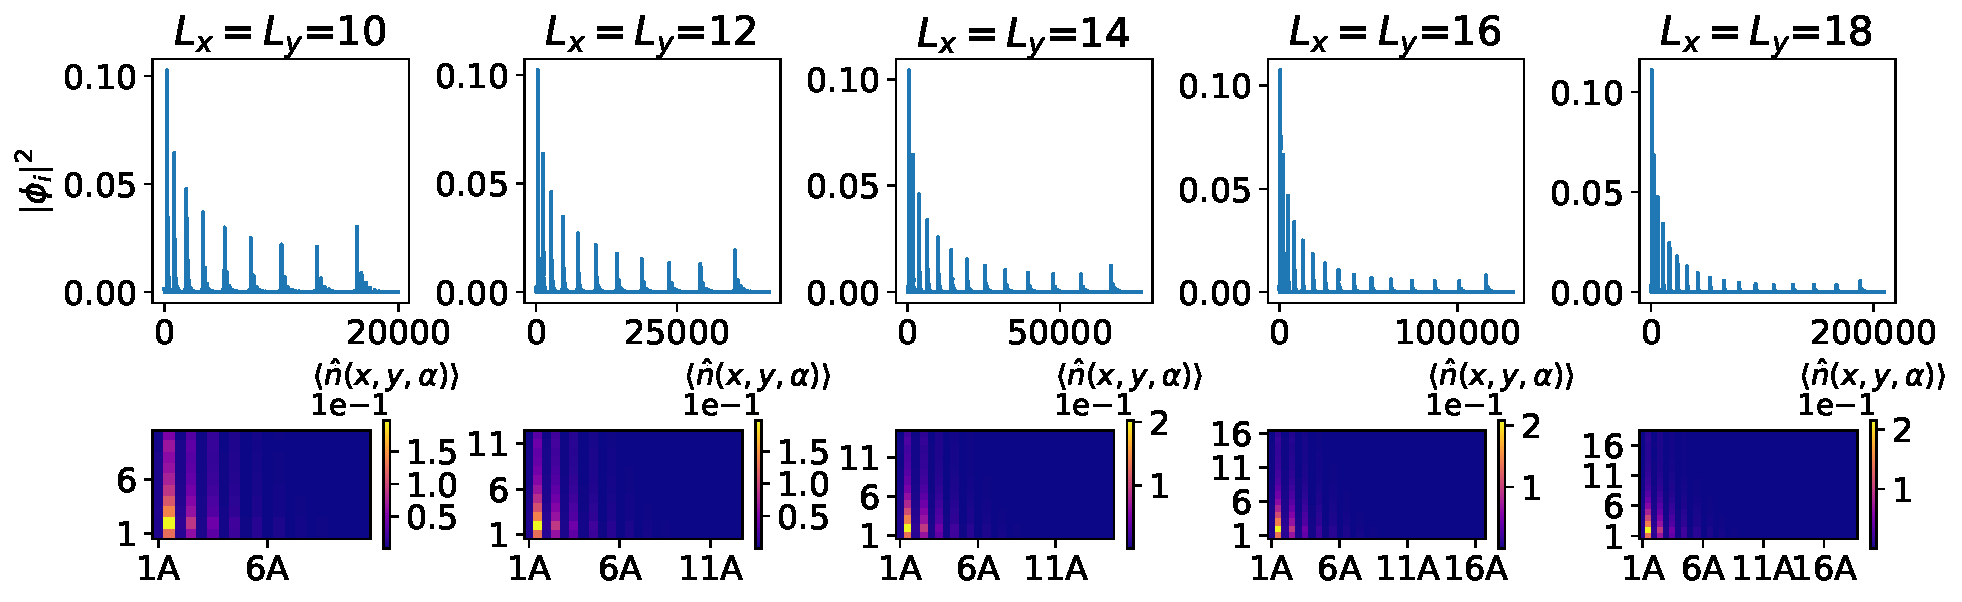
\includegraphics[width=1.\linewidth]{Picture/SI/LargeTwoExcitation.pdf}
		\begin{overpic}[width=1.0\linewidth]{Picture/SI/LargeTwoExcitation_NotTopo.pdf}
			\put(3,61){(a)}
			\put(3,30){(b)}
		\end{overpic}
		\caption{%不同系统尺寸下的本征态和各个格点的粒子数算符平均值$\langle \hat{n}(x,y,\alpha) \rangle$。(a)通过Arnoldi方法计算系统尺寸为$L_x=L_y=[10,12,14,16,18]$的hybrid chiral skin correlated states.在位能为$u=-1.5$，当QWZ模型在不存在多体相互作用时，这个模型是拓扑绝缘体。
		%(b)通过Arnoldi方法计算系统尺寸为$L_x=L_y=[10,12,14,16,18]$的non-Hermitian many-body induced localized states.在位能为$u=-2.1$，当QWZ模型在不存在多体相互作用时，这个模型是拓扑平庸的。
		The probability distribution of eigenstates with the largest imaginary eigenvalue and average particle numbers $\langle \hat{n}(x,y,\alpha) \rangle$ of the eigenstate per lattice site for different system sizes.
		(a) hybrid chiral skin correlated states, calculated with the Arnoldi method, for system sizes $L_x=L_y=[10,12,14,16,18]$. The onsite potential of the QWZ model is $u=-1.5$ and the QWZ model is a topological insulator.
		(b) Non-Hermitian many-body induced localized states, calculated with the Arnoldi method, for system sizes $L_x=L_y=[10,12,14,16,18]$. 
		The onsite potential of the QWZ model is $u=-2.1$ and the QWZ model is a topologically trivial.
		}
		\label{fig:14}
	\end{figure*}
	\begin{figure}[h]
		\centering
		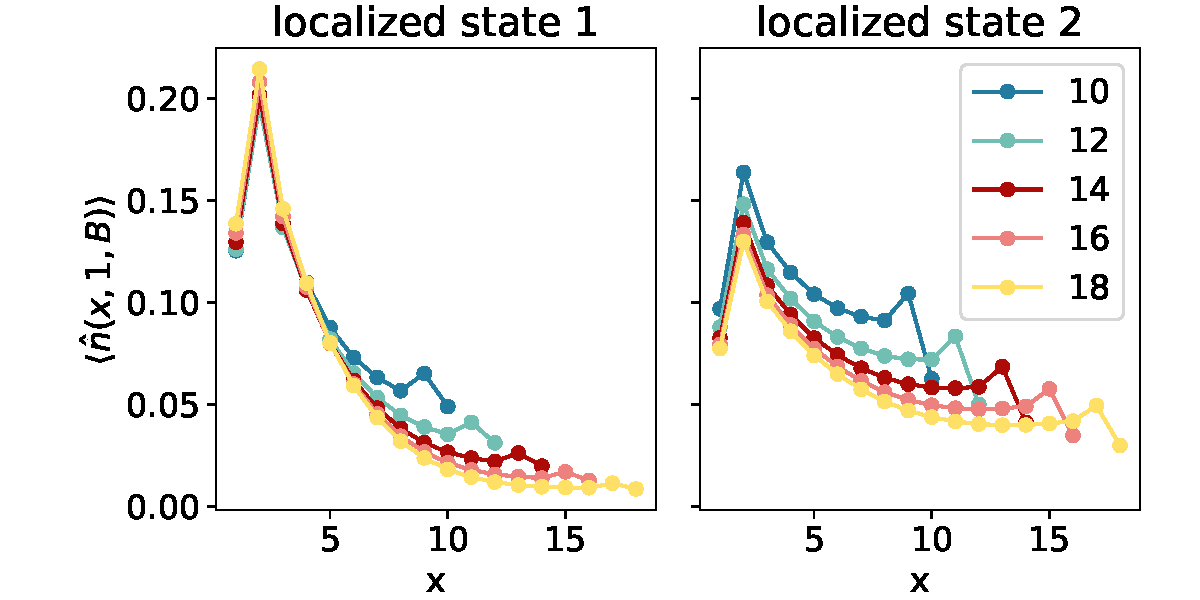
\includegraphics[width=1.\linewidth]{Picture/SI/SI_Comp1.pdf}
		% 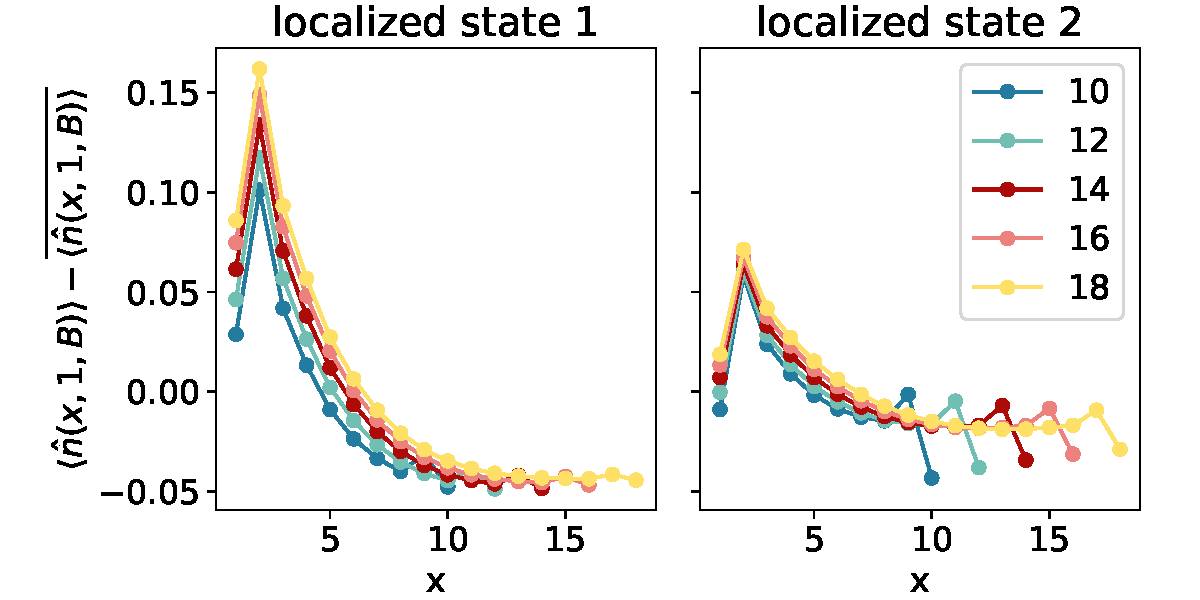
\includegraphics[width=1.\linewidth]{Picture/SI/SI_Comp2.pdf}
		\begin{overpic}[width=1.0\linewidth]{Picture/SI/SI_Comp2.pdf}
			\put(6,98){(a)}
			\put(54,98){(b)}
			% \put(7,54){(c)}
			\put(6,48){(c)}
			\put(54,48){(d)}
		\end{overpic}
		\caption{%不同$x$坐标，$y=1$的$B$子格点的粒子数算符平均值$\langle \hat{n}(x,1,B) \rangle$以及粒子数算符平均值与平均值的差$\langle \hat{n}(x,1,B) \rangle - \overline{\langle \hat{n}(x,1,B) \rangle}$。hybrid chiral skin correlated states，标记为localized state 1，的(a)粒子数算符平均值$\langle \hat{n}(x,1,B) \rangle$和(b)粒子数算符平均值和平均值的差$\langle \hat{n}(x,1,B) \rangle - \overline{\langle \hat{n}(x,1,B)\rangle}$。non-Hermitian many-body induced localized states，标记为localized state 2,的(a)粒子数算符平均值$\langle \hat{n}(x,1,B) \rangle$和(b)粒子数算符平均值和平均值的差$\langle \hat{n}(x,1,B) \rangle - \overline{\langle \hat{n}(x,1,B) \rangle}$。
		Average particle number $\langle \hat{n}(x, 1, B) \rangle $ and the deviations from the average $\langle \hat{n}(x, 1, B) \rangle - \overline{\langle \hat{n}(x, 1, B) \rangle}$ for the B sublattice at $y = 1$ boundary. 
		(a) The average particle number and the deviations from the average of the hybrid chiral skin correlated states (localized state 1). The $x$-axis is the location of the unit cell in the $x$ direction.
		(b) The average particle number and the deviations from the average of non-Hermitian many-body induced localized states (localized state 2).  The $x$-axis is the location of the unit cell in the $x$ direction.
		}
		\label{fig:15}
	\end{figure}
	The QWZ model is a topological insulator and exhibits edge states when the onsite energy $u$ lies within the range $-2 < u < 0$ and $0 < u < 2$. However, when the onsite energy is $u = -2.1$, the QWZ model is topologically trivial, and there are no edge states. 
	We apply gain to the boundary of a topologically trivial insulator and investigate whether multi-particle chiral skin modes and non-Hermitian many-body induced localized states can still arise.
	We study the hybrid chiral skin correlated states and non-Hermitian many-body induced localized states in larger system sizes. 
	% 我们研究具有chiral skin mode的模型($u=-1.5$)和不具有chiral skin mode的模型($u=-2.1$)。当$u=-1.5$时，QWZ模型是拓扑绝缘体，当$u=-2.1$时，QWZ模型是拓扑平庸的。当引入元胞间相互作用$\hat{H}_{\text{inter}}$的时候，具有chiral skin mode的模型会出现hybrid chiral skin correlated states, 不具有chiral skin mode的模型会出现non-Hermitian many-body induced localized states.
	% 我们已经通过精确对角化的方法说明了，在系统尺寸到$L_x=L_y=9$时这样的localized states会存在。接下来我们采用Arnoldi方法说明在更大的系统尺寸下，本征值虚部最大的本征态仍然存在上述局域量子态。
	% hybrid chiral skin correlated states 在更大系统尺寸的本征态以及该本征态在各个格点的粒子数平均值如Fig.~\ref{fig:14}(a)，non-Hermitian many-body induced localized在更大系统尺寸的本征态以及该本征态在各个格点的粒子数平均值如Fig.~\ref{fig:14}(b)所示。从Fig.~\ref{fig:14}中可以发现在更大系统尺寸下，局域量子态仍然存在，同时hybrid chiral skin correlated states更加局域。
	We investigate the QWZ model with and without chiral skin modes, corresponding to onsite energies $u=-1.5$ and $u=-2.1$, respectively. The former is a topological insulator, while the latter is a trivial insulator. When inter-cell interactions $\hat{H}_{\text{inter}}$ are introduced, the model with chiral skin modes exhibits hybrid chiral skin correlated states, while the model without chiral skin modes exhibits non-Hermitian many-body induced localized states.
	We have shown that such localized states exist for system sizes up to $L_x = L_y = 9$ with exact diagonalization method. To explore the localization in larger systems, we employ the Arnoldi method to compute the eigenstate with the largest imaginary eigenvalue. 
	We find that this eigenstate exhibits localization.
	The probability distribution of eigenstates and the average particle number of eigenstates for the hybrid chiral skin correlated states in larger systems are shown in Fig.\ref{fig:14} (a). 
	The probability distribution of eigenstates and the average particle number of eigenstates for non-Hermitian many-body induced localized states are shown in Fig.\ref{fig:14} (b). The results in Fig.~\ref{fig:14} show that these localized states still exist even in larger systems. Moreover, the hybrid chiral skin correlated states are more localized.

	% 我们同时研究在不同系统尺度下，hybrid chiral skin correlated states(labeled as localized state 1)和non-Hermitian many-body induced localized states(labeled as localized state 2)沿着$x$方向，$y$坐标为$y=1$的B晶格的粒子数平均值$\langle \hat{n}(x,y,\alpha) \rangle$以及粒子数平均值与平均值的差$\langle \hat{n}(x,y,\alpha) \rangle - \overline{\langle \hat{n}(x,y,\alpha) \rangle}$。
	% 结果显示，localized state 1的峰值大小不随着系统尺寸的增加而减小，而localized state 2的峰值大小会随着系统尺寸的增加而减小，如Fig.~\ref{fig:15}所示，Fig.~\ref{fig:15}(a)中的现象比Fig.~\ref{fig:15}(b)更具有局域性特征。
	% 此外，从Fig.~\ref{fig:15}(c)和(d)中可以看出，粒子数算符平均值和平均值的差的峰值在localized state 1中随系统尺寸的增加而增加，而localized state 2中不随系统尺寸的变化而变化。
	% 这是因为hybrid chiral skin correlated states是多体相互作用使得本来局域在corner上的chiral skin mode在格点上由于能级差进一步局域化。而non-Hermitian many-body induced localized states仅是由于多体相互作用和非厄米导致的，因此并不如hybrid chiral skin correlated states局域化。

	We further investigate the behavior of hybrid chiral skin correlated states (labeled as localized state 1) and non-Hermitian many-body induced localized states (labeled as localized state 2) at different system sizes. Specifically, we study the average particle number $\langle \hat{n}(x, y, \alpha) \rangle$ and the deviation from average $\langle \hat{n}(x, y, \alpha) \rangle - \overline{\langle \hat{n}(x, y, \alpha) \rangle}$ along the $x$-direction for the $B$ sublattice at $y = 1$ boundary.
	As shown in Fig.~\ref{fig:15}, the peak amplitude of localized state 1 does not decrease as the system size increases, whereas the peak amplitude of localized state 2 decreases as the system size increases. This indicates that the behavior shown in Fig.\ref{fig:15} (a) is more localized than that in Fig.~\ref{fig:15} (b).
	Moreover, Fig.~\ref{fig:15} (c) and Fig.~\ref{fig:15} (d) reveal that the peak values of the deviation from average increases as system size increases for localized state 1, but remain nearly constant for localized state 2.
	hybrid chiral skin correlated states originate from many-body interactions that enhance the localization of topological corner states. 
	The energy splitting induced by many-body interactions further localizes these modes along both directions and confines them to the $B$ sublattice.
	In contrast, non-Hermitian many-body induced localized states arise from the combined effects of non-Hermiticity and many-body interactions. These states do not depend on the presence of localized topological corner state, called chiral skin modes, and therefore exhibit comparatively weaker localization.

	\subsection{The gain sites are not at the boundary}
	% \subsection{Robust to the location of dissipative sites}

	% chiral skin mode是在耗散元胞位于晶格边界时出现的。当拓扑绝缘体的边缘态具有有限的寿命时，手性皮肤模式会出现。
	% 当耗散元胞不位于晶格边界时候，不存在chiral skin mode。当引入多体相互作用的时候，并不会出现hybrid chiral skin correlated states, 而是会出现non-Hermitian many-body induced localized states.
	% % 这二者的区别在于局域程度不同。
	% % beyond topological transition.
	% %在这里，我们阐明NHMBL并非简单的多体chiral skin effect。
	% 当系统的体中存在增益的时候，non-Hermitian many-body induced localized states依然存在，且量子态并不是局域化在系统边界。
	% %实际上当系统的体中存在增益的时候，NHMBL依然存在，且量子态并不会局域化在系统边界。
	% 我们考虑一个$L_x=L_y=9$的二维系统，且增益施加在$y=3$的所有元胞上，包含和不包含多体相互作用的非厄米哈密顿量的能谱和本征态分别展示在Fig.~\ref{fig:10}的第一列和第二列。Fig.~\ref{fig:10}的结果表明，在没有多体相互作用的情况下，因非厄米增益未作用于边缘态，所以此时并未出现局域化的chiral skin mode，虚本征值最大的本征态变为了bulk state，如图Fig.~\ref{fig:10} (e)所示。当存在多体相互作用时，由于相互作用引起的能级差以及非厄米pumping的共同作用，non-Hermitian many-body induced localized states得以存在，并且此时量子态局域化于$y=3$元胞的$B$子晶格。

	Chiral skin modes emerge when gain/loss unit cells are located at the boundaries of the lattice. 
	% These modes arise in topological insulators when edge states possess finite lifetimes.
	In contrast, when the gain is placed away from the lattice edges, chiral skin modes do not appear. In such cases, the introduction of many-body interactions does not lead to hybrid chiral skin correlated states, but instead gives rise to non-Hermitian many-body induced localized states. 
	Notably, the non-Hermitian many-body induced localized states exist even when gain is applied into the bulk of the system, and the eigenstates are not localized at the system's boundary.
	We consider a two-dimensional system of size $L_x = L_y = 9$, where gain is applied to the unit cells at $y = 3$. 
	The spectrum and eigenstates of the non-Hermitian Hamiltonians with or without $\hat{H}_{\text{inter}}$ many-body interactions are shown in Figs.~\ref{fig:10} (a) and (b), respectively. 
	The results in Fig.\ref{fig:10} indicate that no localized chiral skin modes emerge without interaction, since gain is not applied to the edge of the systems. 
	In absence of many-body interaction, the eigenstate with the largest imaginary eigenvalue is a bulk state, as shown in Fig.~\ref{fig:10}(a3). However, when many-body interactions are present, the interaction-induced energy difference and non-Hermitian pumping give rise to non-Hermitian many-body induced localized states. In this case, the eigenstate localize at the $B$ sublattice of the unit cells at $y = 3$.
	\begin{figure}[h]
		\centering
		\begin{overpic}[width=1.0\linewidth]{Picture/SI/SI_TwoExcitationSpectrum_NotEdge.pdf}
			\put(4,97){(a1)}
			\put(42,97){(b1)}
			% \put(7,54){(c)}
			\put(4,62){(a2)}
			\put(42,62){(b2)}
			\put(4,26){(a3)}
			\put(42,26){(b3)}
		\end{overpic}
		%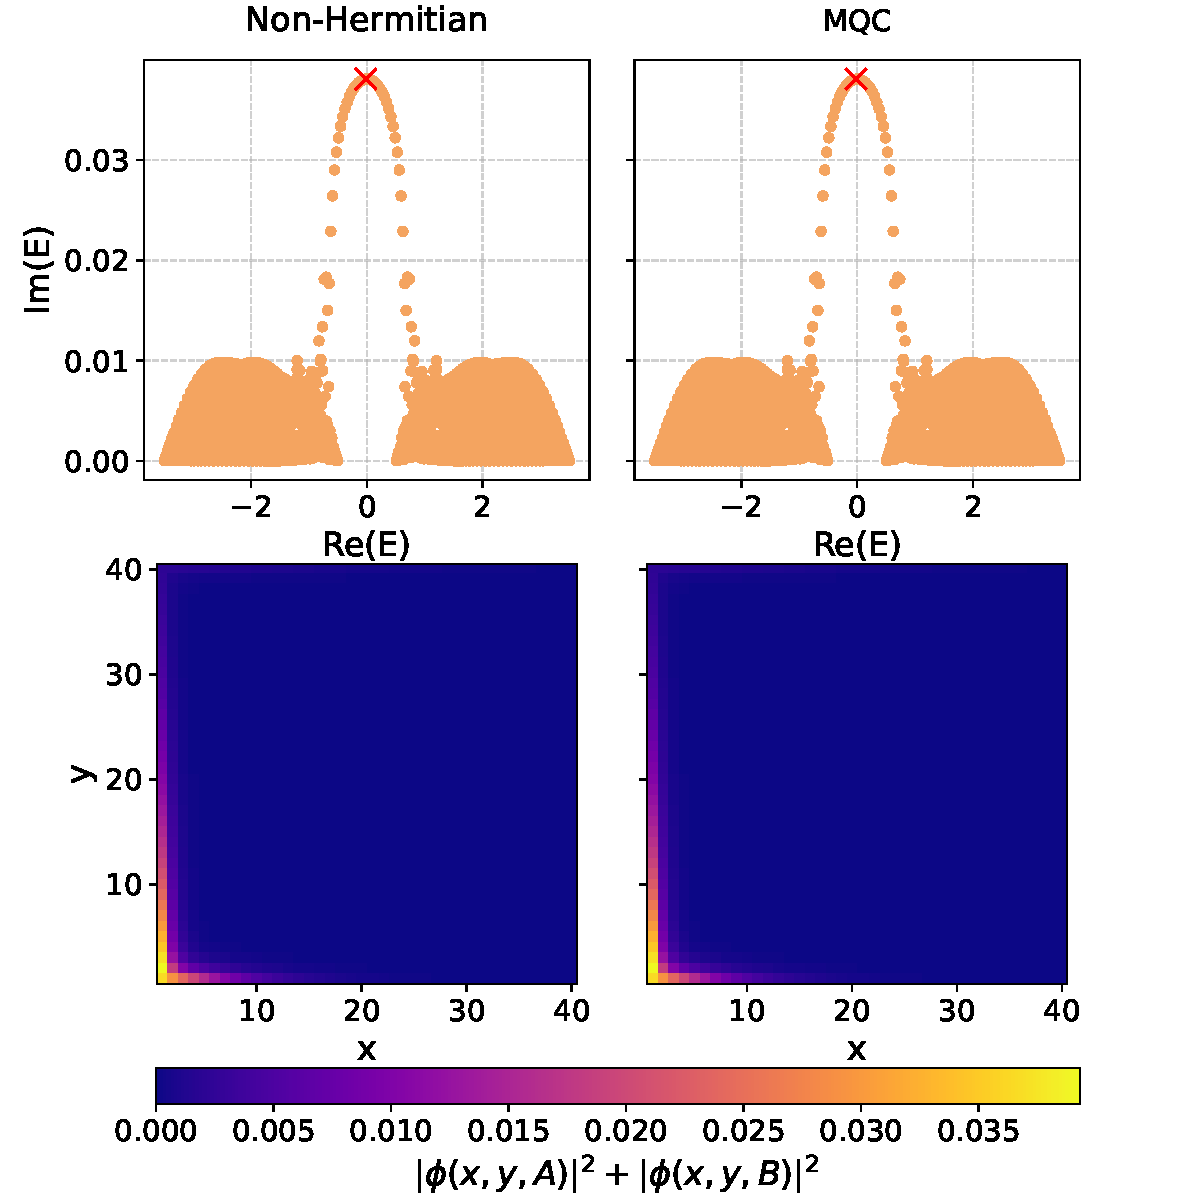
\includegraphics[width=1.\linewidth]{Picture/SingleExcitation_Comp.pdf}
		\caption{%       双激发子空间中能谱和本征态对比，$\gamma=0.2$的非厄米增益$\hat{H}_{\text{im}}$作用于$y=3$边界的元胞。(a) 在不存在相互作用和(b) 存在相互作用时的能谱。(c) 在不存在相互作用和(d) 存在相互作用时本征态的模方，其能量在(a)和(b)中用橘色十字表示。(e) (c)中本征态在各个格点的粒子数平均数，该态是多粒子的chiral skin mode。(f) (d)中本征态在各个格点的粒子数平均数，该态是NHMBL。系统尺寸为$L_x=L_y=9$，在位能为$u=-1.5$。
		In the two-excitation subspace, the comparison of spectrum and eigenstates between non-Hermitan Hamiltonian with or without $\hat{H}_{\text{inter}}$ many-body interaction. The gain ($\gamma=0.2$) is applied to unit cells at $y=3$.
		(a1) The spectrum of a non-Hermitian Hamiltonian without interaction.
		(b1) The spectrum of a non-Hermitian Hamiltonian with interaction.
		(b2) The probability distribution of the eigenstates of a non-Hermitian Hamiltonian without interaction.
		(b2) The probability distribution of the eigenstates of a non-Hermitian Hamiltonian with interaction.
		(a3) The average particle number per lattice site for the eigenstate in (a2).
		(b3) The average particle number per lattice site for the eigenstate in (b2), which corresponds to non-Hermitian many-body interactions induced localized states.
		The system size is $L_x=L_y=9$, and the onsite potential is $u=-1.5$.
		}
		\label{fig:10}
	\end{figure} %label from y=1 and x=1?

	% \subsection{When there is no edge states}
	% % \subsection{The NHMBL exists even when there is no edge state}

	% % 由于QWZ模型当$-2<u<0$和$0<u<2$时，模型表现为拓扑绝缘体并存在边缘态。然而，当$u=2.1$时，QWZ模型变为拓扑平庸的绝缘体，此时不再存在edge state。我们考虑对一个拓扑平庸的绝缘体的边界施加增益，并观察是否会出现chiral skin mode和non-Hermitian many-body induced localized states。根据chiral skin effect的理论，对仅存在bulk state的系统施加增益并不会导致chiral skin mode，如Fig.~\ref{fig:11}(e)所示。然而，当我们在没有边缘态的拓扑绝缘体中施加增益和多体相互作用时，non-Hermitian many-body induced localized states会出现(Fig.~\ref{fig:11}(f))，这是因为非厄米pumping和多体相互作用引起的能级差仍然存在。因此它们的共同作用导致了NHMBL的出现。由此可见，non-Hermitian many-body induced localized states的存在并不依赖于厄米哈密顿量是否为拓扑绝缘体，也不依赖于增益是否作用于边缘态。
	% % % 但是该态并不是hybrid chiral skin correlated states, 因为这个态并不是对chiral skin mode引入多体相互作用导致的，所以并不如hybrid chiral skin correlated states局域。
	% % % 对于增益和耗散是否存在对称性？存在，但是如何解释机理呢？从对称性来。
	% % % 增益和耗散是左矢和右矢的区别。

	% The QWZ model is a topological insulator and exhibits edge states when onsite energy $u$ lies within the range $-2 < u < 0$ and $0 < u < 2$. However, when the onsite energy is $u = -2.1$, the QWZ model is topologically trivial, and there is no edge states. 
	% We apply gain to the boundary of a topologically trivial insulator and investigate whether multi-particle chiral skin modes and non-Hermitian many-body induced localized states can still arise.
	% According to the theory of chiral skin effect, applying gain to topologically trivial insulators does not lead to the emergence of chiral skin modes, as shown in Fig.\ref{fig:11} (a3). 
	% However, when both gain and many-body interactions are introduced into the topologically trivial insulators, non-Hermitian many-body induced localized states emerge, as shown in Fig.\ref{fig:11} (b3). This phenomenon arises from the combined effects of non-Hermitian pumping and interaction-induced energy differences.
	% These results demonstrate that the existence of non-Hermitian many-body induced localized states does not rely on the topology of Hermitian Hamiltonian and the localtion of gain unit cells.
	% \begin{figure}[h]
	% 	\centering
	% 	\begin{overpic}[width=1.0\linewidth]{Picture/SI/SI_TwoExcitationSpectrum_NotTopology.pdf}
	% 		\put(4,97){(a1)}
	% 		\put(42,97){(b1)}
	% 		% \put(7,54){(c)}
	% 		\put(4,62){(a2)}
	% 		\put(42,62){(b2)}
	% 		\put(4,26){(a3)}
	% 		\put(42,26){(b3)}
	% 	\end{overpic}
	% 	%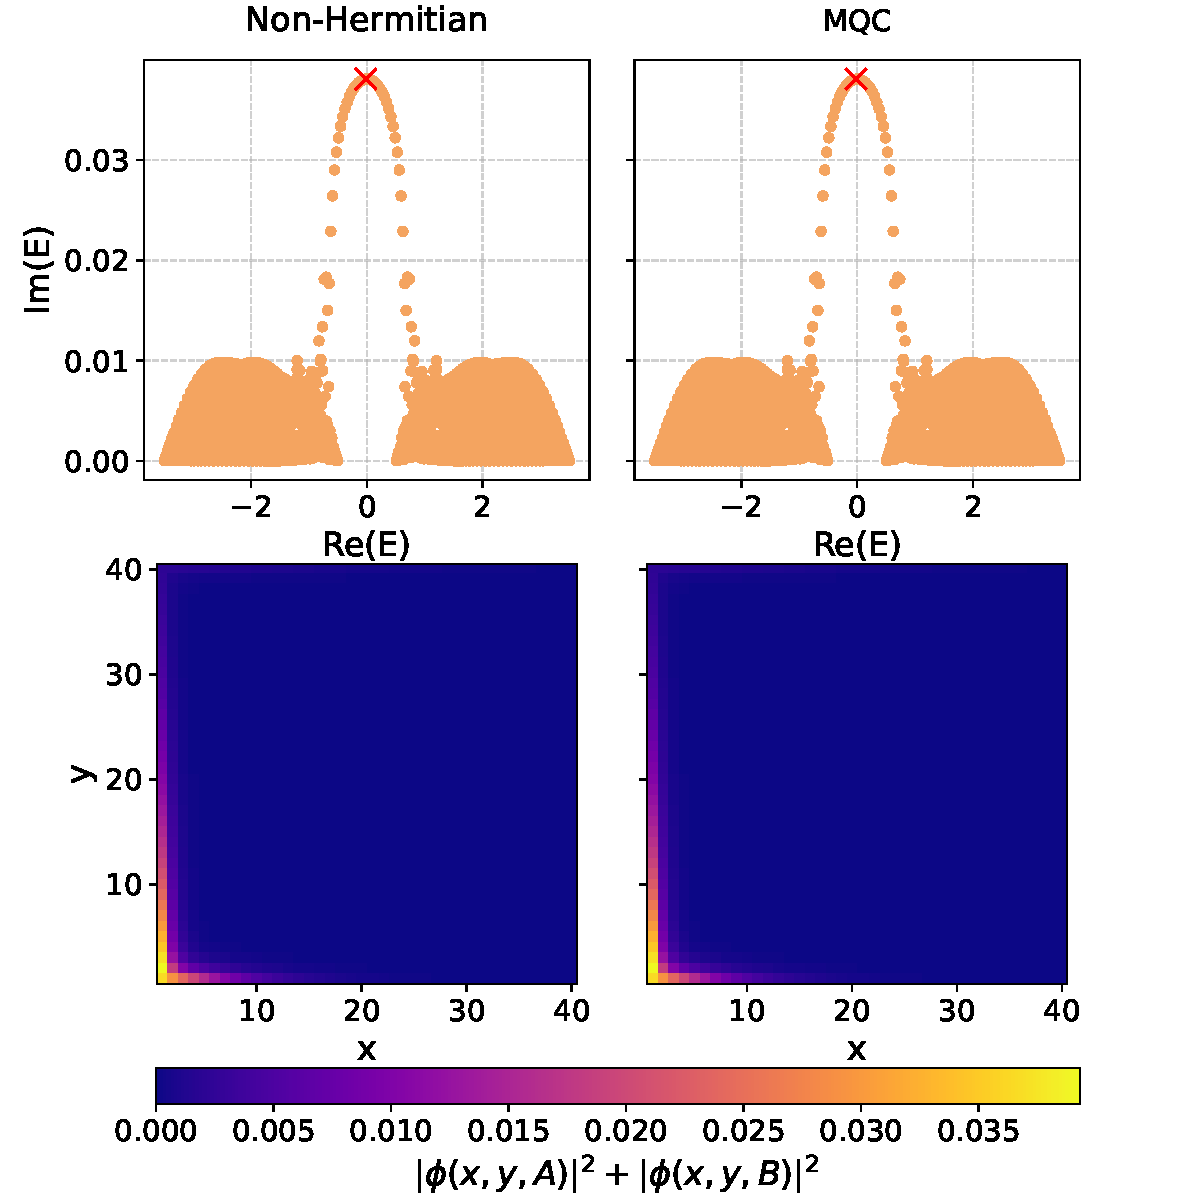
\includegraphics[width=1.\linewidth]{Picture/SingleExcitation_Comp.pdf}
	% 	\caption{%双激发子空间中能谱和本征态对比，$\gamma=0.2$的非厄米增益$\hat{H}_{\text{im}}$作用于$y=1$边界的元胞。(a1) 在不存在相互作用和(b1) 存在相互作用时的能谱。(a2) 在不存在相互作用和(b2) 存在相互作用时本征态的模方，其能量在(a1)和(b1)中用橘色十字表示。(a3) (a2)中本征态在各个格点的粒子数平均数，该态是多粒子的chiral skin mode。(b3) (b2)中本征态在各个格点的粒子数平均数，该态是NHMBL。系统尺寸为$L_x=L_y=9$，在位能为$u=-2.1$，此时QWZ模型是拓扑平庸的。 
	% 	In the two-excitation subspace, the comparison of spectrum and eigenstates between non-Hermitan Hamiltonian with or without $\hat{H}_{\text{inter}}$ many-body interaction. The gain ($\gamma=0.2$) is applied to unit cells at the $y=1$ boundary.
	% 	(a1) The spectrum of non-Hermitian Hamiltonian without interaction.
	% 	(b1) The spectrum of non-Hermitian Hamiltonian with interaction.
	% 	(a2) The probability distribution of eigenstates of non-Hermitian Hamiltonian without interaction.
	% 	(b2) The probability distribution of eigenstates of non-Hermitian Hamiltonian with interaction.
	% 	(a3) The average particle number per lattice site for the eigenstate in (a2).
	% 	(b3) The average particle number per lattice site for the eigenstate in (b2), which corresponds to non-Hermitian many-body induced localized states.
	% 	The system size is $L_x=L_y=9$, and the onsite potential is $u=-2.1$.
	% 	}
	% 	\label{fig:11}
	% \end{figure} %label from y=1 and x=1?
	
	% % \section{NHMBL with intra cell interaction\label{sec:NHMBL_intra}}

	% % 在上述讨论中，我们主要考虑了多体相互作用$\hat{H}_{\text{inter}}$的情况。接下来，我们将探讨在其它类型的相互作用下，chiral skin mode和NHMBL是否存在。我们仅考虑元胞内$A$子格点和$B$子格点之间的粒子相互作用，形式为
	% % \begin{equation}
	% % 	\hat{H}_{\text{intra}} = \sum_{{x}=1}^{L_{x}-1} \sum_{{y}=1}^{L_{y}}  U_{\text{intra}} \hat{n}_{{x}, {y}, A} \hat{n}_{{x}, {y}, B}.
	% % \end{equation}
	% % 我们考虑一个$L_x=L_y=9$的二维系统，且增益施加在$y=1$的所有元胞上。相应的结果展示在Fig.~\ref{fig:12}中。在相互作用强度$U_{\text{intra}}=1.0$的情况下，虽然本征态和本征值的形式与无多体相互作用时有所不同，利用粒子数算符描述多粒子的chiral skin mode仍然存在。这是因为多体相互作用$\hat{H}_{\text{intra}}$并未引入$\mathscr{H}_{\text{gain}}$空间中所有态与其它态之间的能级差，被pumping到该空间的粒子会有相当一部分通过跃迁的方式离开该空间，从而导致由于边缘态引起的chiral skin effect的出现，而不会导致NHMBL的出现。
	% % \begin{figure}[h]
	% % 	\centering
	% % 	\begin{overpic}[width=1.0\linewidth]{Picture/SI/SI_TwoExcitationSpectrum_intra.pdf}
	% % 		\put(4,97){(a)}
	% % 		\put(42,97){(b)}
	% % 		% \put(7,54){(c)}
	% % 		\put(4,62){(c)}
	% % 		\put(42,62){(d)}
	% % 		\put(4,26){(e)}
	% % 		\put(42,26){(f)}
	% % 	\end{overpic}
	% % 	%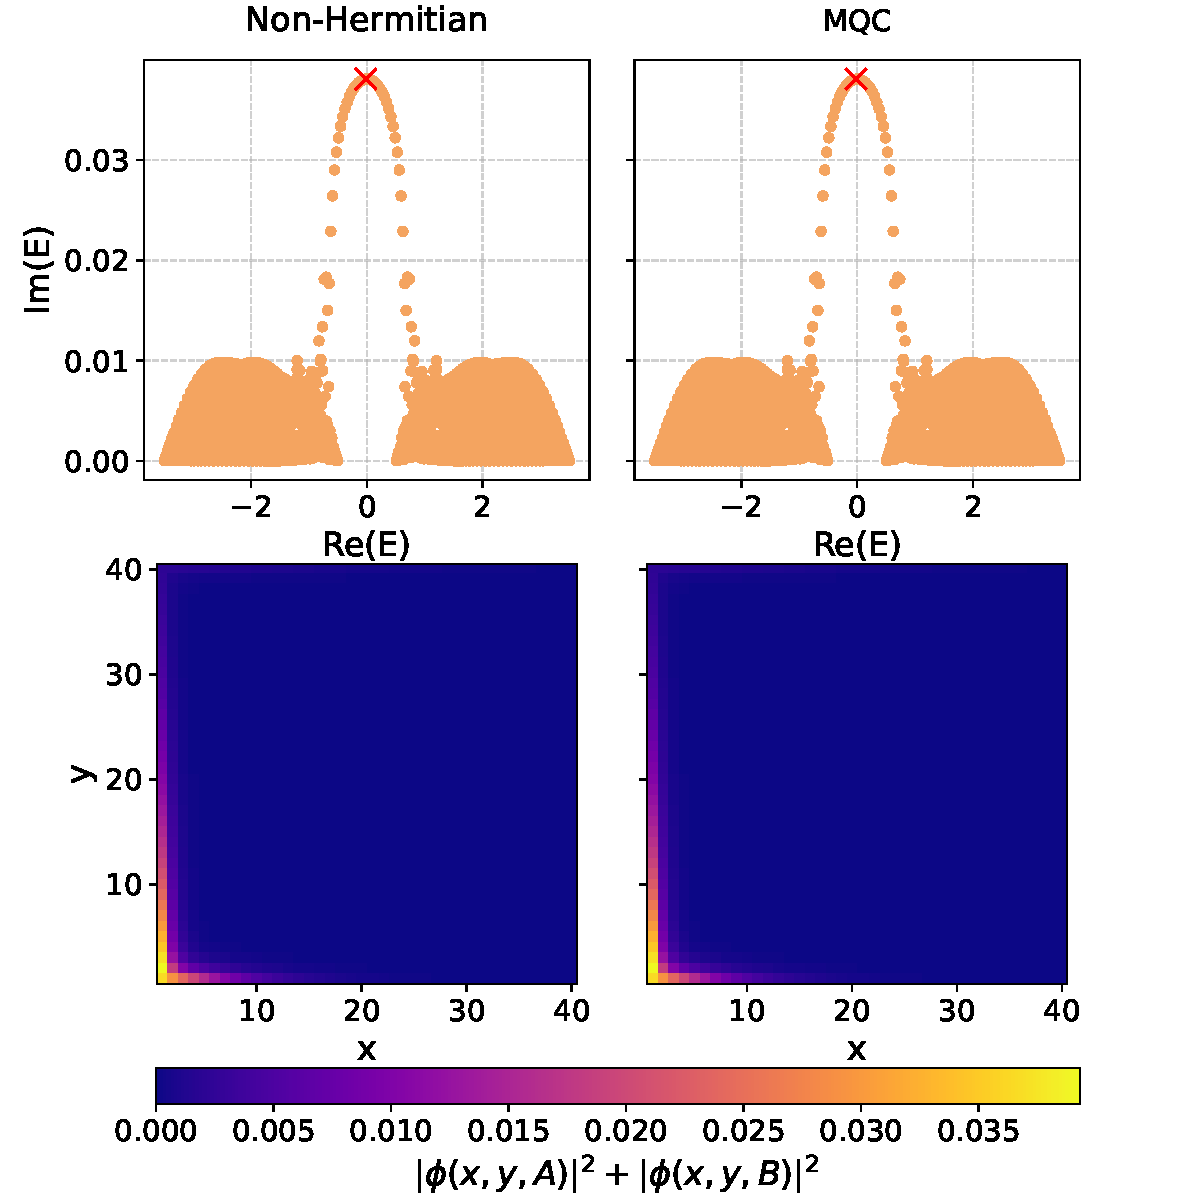
\includegraphics[width=1.\linewidth]{Picture/SingleExcitation_Comp.pdf}
	% % 	\caption{双激发子空间中能谱和本征态对比。$\gamma=0.2$的非厄米增益$\hat{H}_{\text{im}}$作用于$y=1$边界的元胞，多体相互作用为$\hat{H}_{\text{intra}}$。(a) 在不存在相互作用和(b) 存在相互作用时的能谱。(c) 在不存在相互作用和(d) 存在相互作用时本征态的模方，其能量在(a)和(b)中用橘色十字表示。(e) (c)中本征态在各个格点的粒子数平均数，该态是多粒子的chiral skin mode。(f) (d)中本征态在各个格点的粒子数平均数，该态是NHMBL。系统尺寸为$L_x=L_y=9$，在位能为$u=-1.5$。}
	% % 	\label{fig:12}
	% % \end{figure} %label from y=1 and x=1?

	
	\section{The $\mathcal{P}_{x,y,\alpha}$ at different interaction strengths~\label{sec:AllP}}

	% Fig.~\ref{fig:17_2} (a1) shows the energy spectrum in the two-excitation subspace for the non-Hermitian many-body Hamiltonians with a system size of $L_x=L_y=7$. In Fig.~\ref{fig:17_2} (a2), the probability distribution of the eigenstate with the largest imaginary eigenvalue (orange cross in Fig.~\ref{fig:17_2}) is shown. This eigenstate typically dominates the long-time dynamics governed by non-Hermitian many-body Hamiltonians. Fig.~\ref{fig:17_2} (a3) shows the average particle number $\langle \hat{n}(x,y,\alpha) \rangle$ at each lattice site for the eigenstate. The results show that the hybrid chiral skin correlated states exist in system size $L_x=L_y=7$. 
	\begin{figure}[h]
		\centering
		\begin{overpic}[width=1.0\linewidth]{Picture/SI/SI_EvolveSpectrum2.pdf}
			\put(5,81){(a1)}
			\put(54,81){(a2)}
			\put(5,35){(a3)}
		\end{overpic}
		\caption{
		The spectrum and eigenstate in two-excitation subspace. The non-Hermitian gain ($\gamma=0.2$) is applied to unit cells at the $y=1$ boundary, and the many-body interaction is $\hat{H}_{\text{inter}}$. The system size for (a1-a3) is $L_x=L_y=7$. The onsite potential is $u=-1.5$.
		(a1) The spectrum of non-Hermitian many-body Hamiltonian.
		(a2) The probability distribution of the eigenstate of a non-Hermitian many-body Hamiltonian. 
		(a3) The average particle number per lattice site for the eigenstate.
		}
		\label{fig:17_2}
	\end{figure} %label from y=1 and x=1?

	The distinct spectral feature is also observable in digital quantum simulations. In Fig.~\ref{fig:02_Supple}, we analyze the localization dynamics within the two-excitation subspace. At this point, we choose the system size $L_x=L_y=7$, whose spectrum is similar to that in Fig.~\ref{fig:02} (a) ($L_x=L_y=9$). The spectrum and the eigenstate with the largest imaginary eigenvalue are shown in Fig.~\ref{fig:17_2}
	%
	To study the hybrid chiral skin correlated states in different interaction strength $U_{\text{inter}}$, we introduce a measurable quantity which is compatible with the MQCs. % 我们定义了一种适合于量子电路监测的量度。
	We begin with random excitation of two lattice sites to
	% by randomly exciting two lattice sites of the system to 
	study the time evolution of both the non-Hermitian Hamiltonian without and with the many-body interaction $\hat{H}_{\text{inter}}$. 
	% This evolution is implemented using the quantum circuit depicted in Fig.~\ref{fig:01}(a). 
	Subsequently, at time $t=60$, we measure the average particle number $\langle \psi_{t} \vert \hat{n}_{x,y,\alpha} \vert \psi_t \rangle$ of the final state $\psi_t$ at each lattice site ($\alpha=A,B$). We take the average over $N_{\text{samp}}=10^4$ experiments and statistically analyze the number of eventss where the expectation value $\langle \psi_{t} \vert \hat{n}_{x,y,\alpha} \vert \psi_t \rangle$ exceeds $1/(2L_x)$ at each lattice site
	\begin{equation}
		\mathcal{P}_{{x}, {y}, {\alpha}} = \sum^{N_{\text{samp}}} \mathbb{I}(\langle \psi_{t} \vert \hat{n}_{x,y,\alpha} \vert \psi_t \rangle > \frac{1}{2L_x}), \label{eq:NumbEvent}
	\end{equation}
	where $\mathbb{I}(X)$ is the indicator function, which is 1 (0) when $X$ is true (false).% 其中，$\mathbb{I}(X)$是指示函数，当$X$为真时取值为1，否则取值为0。
	% Results demonstrate that, under the many-body Hermitian Hamiltonian, starting from any localized two-excitation quantum state, the event counts $\mathcal{P}_{x,y,\alpha}$ at lattice site $(x,y,\alpha)$ at times $t=20$ and $t=60$ decrease as the interaction strength $\vert U_{\text{inter}} \vert$ increases. This indicates that, with stronger interactions, quantum states evolve toward less localized states.
	Our results demonstrate distinct localization behaviors under Hermitian and non-Hermitian many-body Hamiltonians. For the Hermitian case, when the system starts from an arbitrary localized two-excitation quantum state, the number of events $\mathcal{P}_{x,y,\alpha}$ at times $t=60$ exhibit a decreasing trend with increasing interaction strength $\vert U_{\text{inter}} \vert$. This suggests that stronger interactions drive the system toward delocalized states.
	In contrast, for the non-Hermitian case, the number of events $\mathcal{P}_{x,y,\alpha}$ at unit cell $(x,y)=(1,3)$ decreases with increasing interaction strength. the number of events at unit cells $(x,y)=(1,1),(1,2)$ first decreases and then increases (Fig.~\ref{fig:02_Supple}). 
	Therefore, the stronger many-body interaction can drive the system toward localized states in the presence of non-Hermiticity.
	This behavior is attributed to the presence of hybrid chiral skin correlated states, which ensure that regardless of the initial state, the system ultimately evolves into localized states and can be detected.
	When evolving from a random two-particle excited state, the system exhibits localization signals at the $B$ sites of the gain unit cells at time $t=60$.
	In about $88\%$ of the cases, the average particle number at one or more sites exceeds $1/(2L_x)$ (solid lines in Fig.~\ref{fig:02_Supple}).
	% A detailed analysis of $\mathcal{P}_{x,y,\alpha}$ for all lattice sites is provided in Appendix~\ref{sec:AllP}, which also supports the discussion here. 
	\begin{figure}[htbp]
		\begin{overpic}[width=0.95\linewidth]{picture2/Popu_Interaction.pdf}
		\end{overpic}
		% \begin{minipage}[b]{0.47\textwidth}
		% 	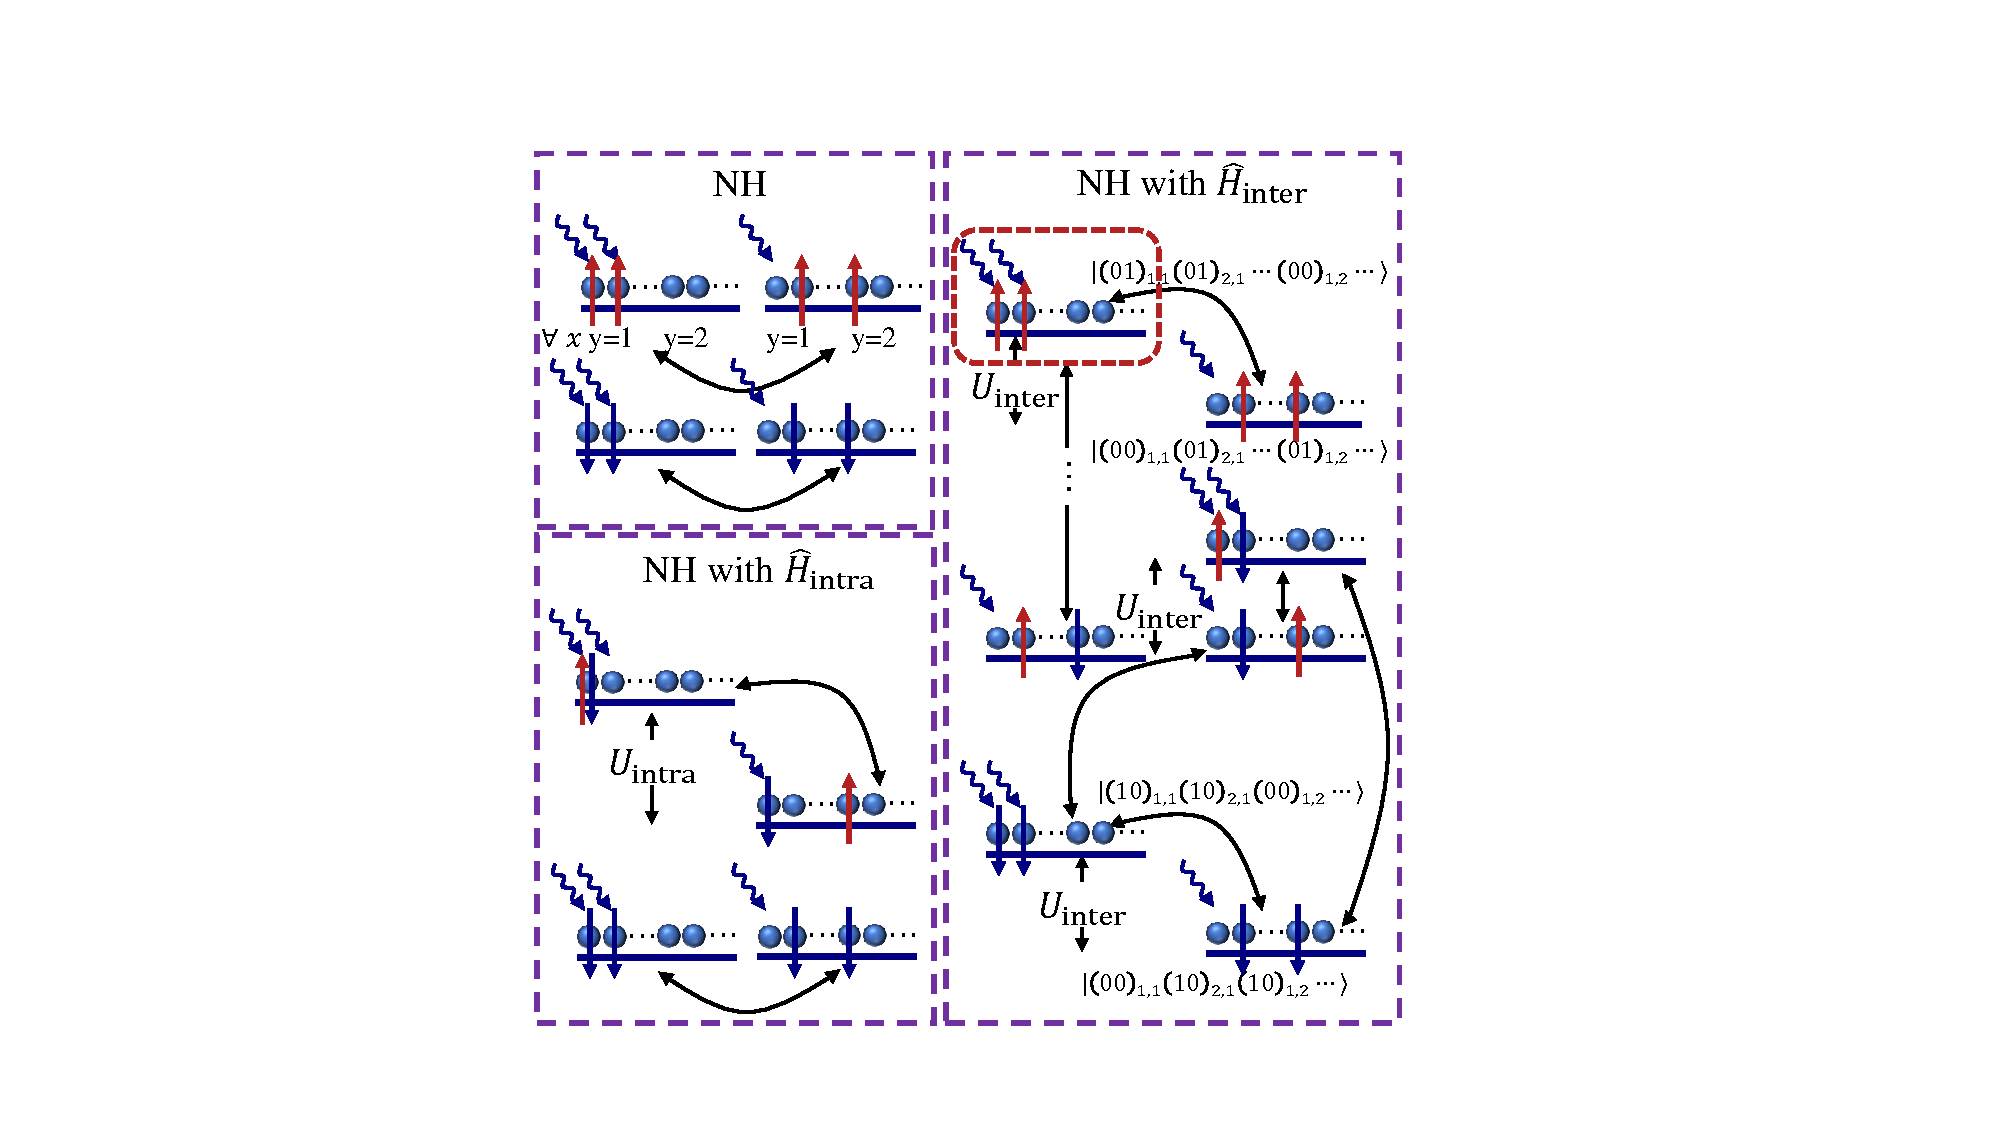
\includegraphics[width=\textwidth]{Picture/Mechanism_inter.pdf}
		% 	% \caption{图片3说明}
		% 	% \label{fig:img3}
		% \end{minipage}
		% \begin{overpic}[width=0.49\linewidth]{Picture/Popu_Interaction.pdf}
		% 	\put(-96,152){(a)}
		% 	% \put(7,54){(c)}
		% 	\put(-96,99){(b)}
		% 	\put(2,99){(c)}
		% 	% \put(49,54){(d)}
		% \end{overpic}
		\caption{The parameters $\mathcal{P}_{x,y,\alpha}$ at time $t=60$ for the non-Hermitian Hamiltonian with $\hat{H}_{\text{inter}}$ interaction under different interaction strengths. Gain is applied to $y=1$ boundary. The system size is $L_x=L_y=7$, and the onsite potential is $u=-1.5$. The number of randomly selected initial quantum states is $N_{\text{samp}}=10^4$.}
		\label{fig:02_Supple}
	\end{figure}


	%我们研究了在不同时间和相互作用强度$U_{\text{inter}}$下在各个格点处$\mathcal{P}_{x,y,\alpha}$的值。我们分别计算了在哈密顿量$\hat{H}_{\text{QWZ}}+\hat{H}_{\text{inter}}$和$\hat{H}_{\text{QWZ}}+\hat{H}_{\text{inter}}+\hat{H}_{\text{im}}$演化下在时间$t=20$和$t=60$时刻$\mathcal{P}_{x,y,\alpha}$(Fig.~\ref{fig:appendixA_fig01})。结果表明在只存在多体相互作用的时候，所有格点的$\mathcal{P}_{x,y,\alpha}$都随相互作用强度$\vert U_{\text{inter}} \vert$的增加而减小，这表明随着相互作用强度的增加，量子态更趋向于演化向非局域的量子态。
	%而在存在非厄米的时候，部分格点的$\mathcal{P}_{x,y,\alpha}$同样随相互作用强度的增加而减小。但是在部分格点处的$\mathcal{P}_{x,y,\alpha}$随相互作用的增加先减小后增加。
	%这是由于hybrid chiral skin correlated states的存在，导致从任意格点出发的粒子最后都会演化到该局域化的量子态上，从而被探测到。且上面的现象随着时间的增加更加明显，因为此时更加趋向于稳态。

	We then investigate the behavior of $\mathcal{P}_{x,y,\alpha}$ for all lattice sites under different evolution times and interaction strengths $U_{\text{inter}}$. Specifically, we compute $\mathcal{P}_{x,y,\alpha}$ at times $t = 20$ and $t = 60$ under the dynamics governed by the Hamiltonians $\hat{H}_{\text{QWZ}} + \hat{H}_{\text{inter}}$ and $\hat{H}_{\text{QWZ}} + \hat{H}_{\text{inter}} + \hat{H}_{\text{im}}$ (Fig.~\ref{fig:appendixA_fig01}). 
	In the absence of non-Hermitian term, we observe that $\mathcal{P}_{x,y,\alpha}$ at all lattice sites consistently decreases as $\lvert U_{\text{inter}} \rvert$ increases, indicating that stronger interactions drive the system toward more delocalized quantum states. 
	In contrast, when non-Hermitian terms are present, a more intricate behavior emerges: while the parameter $\mathcal{P}_{x,y,\alpha}$ at $y\neq 1$ unit cells still decreases as interaction strength increases, 
	the parameter $\mathcal{P}_{x,y,\alpha}$ at $y=1$ unit cells first decreases then increases as interaction strength increases.
	This phenomenon arises from the emergence of hybrid chiral skin correlated states. The particles evolve to localized states regardless of the initial states. This localized states are then detected at site along $y=1$ boundary. The manifestation of this effect becomes more obvious at longer evolution times, and this effect has potential application in controlling exotic quantum states.
	%reflecting the system's approach toward a steady-state configuration.

	\begin{figure}[h]
		\centering
		%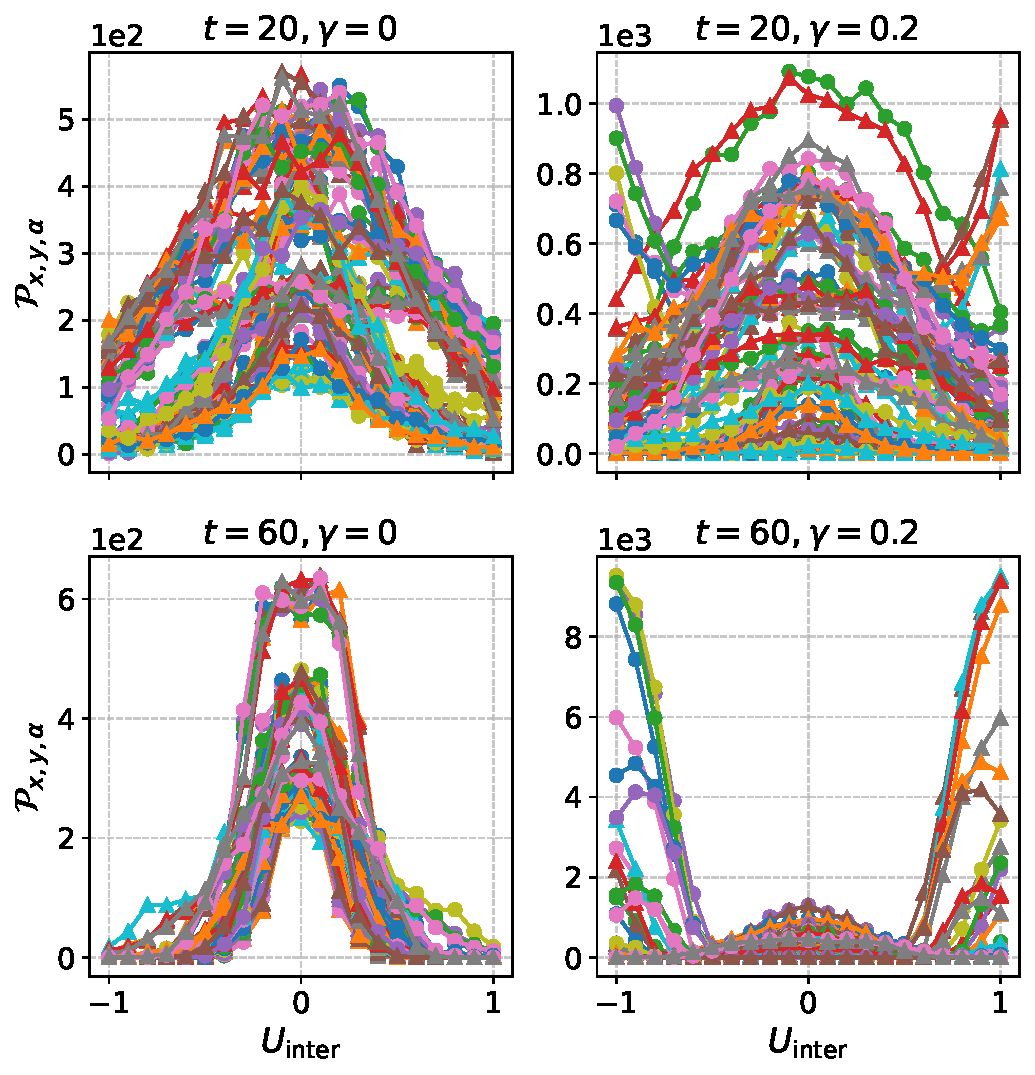
\includegraphics[width=1.\linewidth]{Picture/SI/SI_Popu_Interaction.pdf}
		\begin{overpic}[width=1.0\linewidth]{Picture/SI/SI_Popu_Interaction.pdf}
			\put(3,98){(a)}
			\put(50,98){(b)}
			\put(3,50){(c)}
			\put(50,50){(d)}
			% \put(49,54){(d)}
		\end{overpic}
		\caption{%在时间$t=20$和$t=60$时，不同相互作用强度下的$\mathcal{P}_{x,y,\alpha}$。(a) 在时间$t=20$，不存在非厄米增益的多体哈密顿量。(b) 在时间$t=20$，存在$\gamma=0.2$的$\hat{H}_{\text{im}}$的非厄米多体哈密顿量。(c) 在时间$t=60$，不存在非厄米增益的多体哈密顿量。(d) 在时间$t=60$，存在$\gamma=0.2$的$\hat{H}_{\text{im}}$的非厄米多体哈密顿量。增益作用于$y=1$元胞。系统尺寸为$L_x=L_y=7$，在位能为$u=-1.5$。选取的随机初始量子态数目为$N_{\text{samp}}=10^4$。
		The parameters $\mathcal{P}_{x,y,\alpha}$ at times $t=20$ and $t=60$ under different interaction strengths $U_{\text{inter}}$. The initial quantum state is chosen as an arbitrary two-excitation state.
		(a) The results of many-body Hamiltonian without non-Hermitian gain at time $t=20$. 
		(b) The results of many-body Hamiltonian with non-Hermitian gain $\hat{H}_{\text{im}}$ ($\gamma=0.2$) at time $t=20$. 
		(c) The results of many-body Hamiltonian without non-Hermitian gain at time $t=60$. 
		(d) The results of many-body Hamiltonian with non-Hermitian gain $\hat{H}_{\text{im}}$ ($\gamma=0.2$) at time $t=60$. 
		Gain is applied to the $y = 1$ unit cell. The system size is $L_x=L_y=7$, and the onsite potential is $u=-1.5$. The number of randomly selected initial quantum states is $N_{\text{samp}}=10^4$.
		}
		\label{fig:appendixA_fig01}
	\end{figure}


	\section{The hybrid chiral skin correlated states exist in a dissipative Hamiltonian.~\label{sec:appendicD_loss}}
	\begin{figure}[h]
		\centering
		\begin{overpic}[width=1.0\linewidth]{Picture/SI/SI_TwoExcitationSpectrum_loss.pdf}
			\put(4,97){(a1)}
			\put(44,97){(b1)}
			% \put(7,54){(c)}
			\put(4,62){(a2)}
			\put(44,62){(b2)}
			\put(4,26){(a3)}
			\put(44,26){(b3)}
		\end{overpic}
		%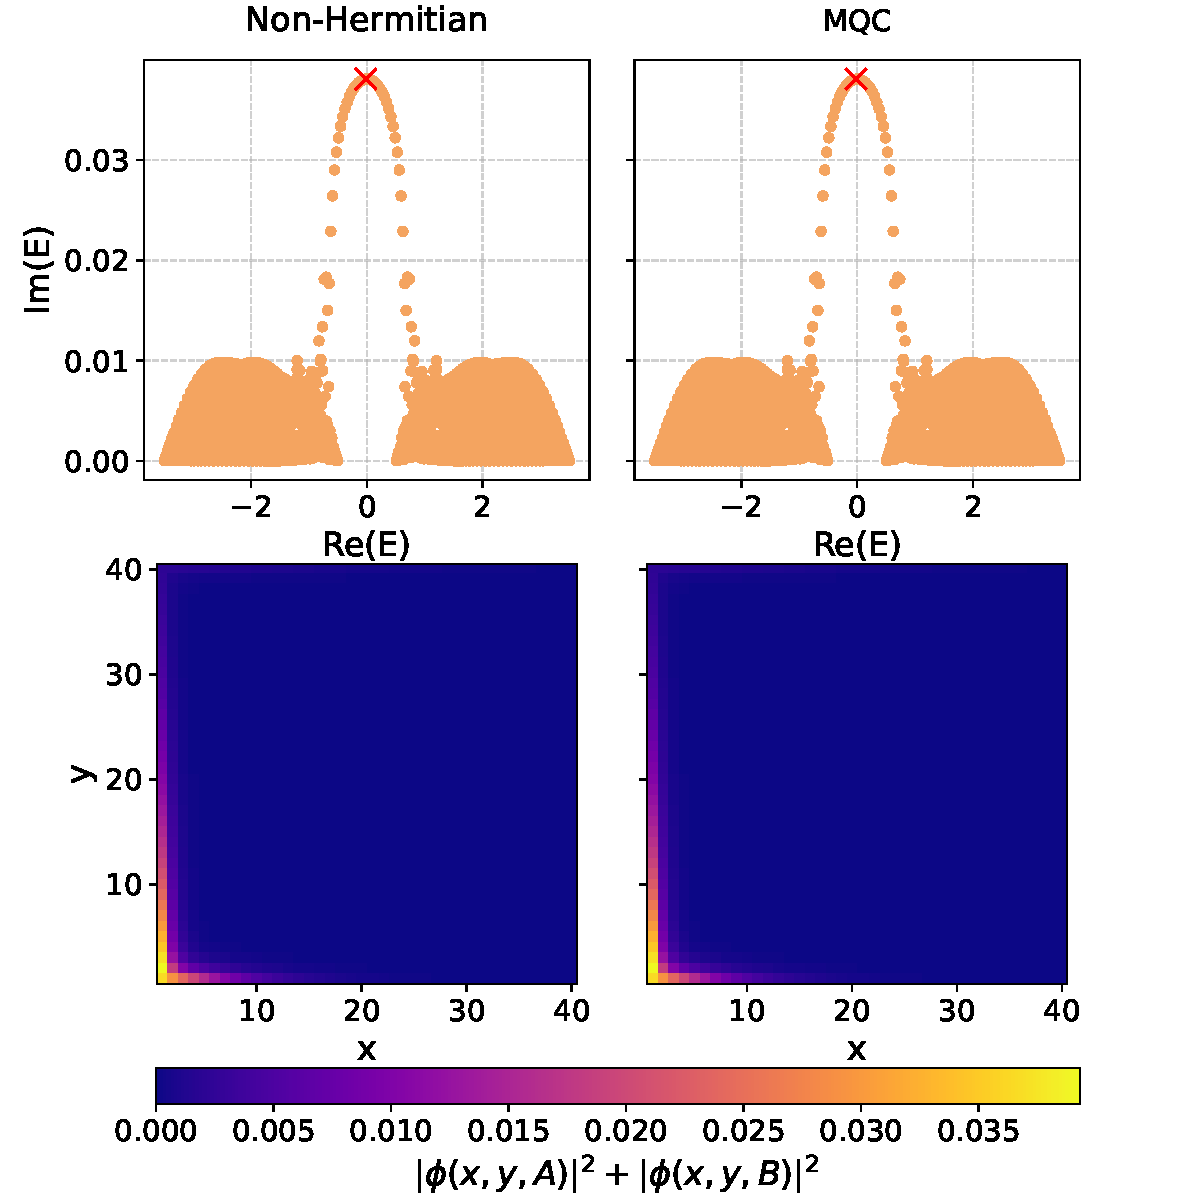
\includegraphics[width=1.\linewidth]{Picture/SingleExcitation_Comp.pdf}
		\caption{%双激发子空间中能谱和本征态对比，$\gamma=-0.2$的非厄米耗散$\hat{H}_{\text{im}}$作用于$y=1$边界的元胞。(a1) 在不存在相互作用和(b1) 存在相互作用时的能谱。(a2) 在不存在相互作用和(b2) 存在相互作用时本征态的模方，其能量在(a1)和(b1)中用橘色十字表示。(a3) (a2)中本征态在各个格点的粒子数平均数，该态是多粒子的chiral skin mode。(b3) (b2)中本征态在各个格点的粒子数平均数，该态是NHMBL。系统尺寸为$L_x=L_y=9$，在位能为$u=-1.5$。
		In the two-excitation subspace, the comparison of spectrum and eigenstates between non-Hermitan Hamiltonian with or without $\hat{H}_{\text{inter}}$ many-body interaction. The non-Hermitian dissipation ($\gamma=-0.2$) is applied to unit cells at the $y=1$ boundary.
		(a1) The spectrum of a non-Hermitian Hamiltonian without interaction.
		(b1) The spectrum of a non-Hermitian Hamiltonian with interaction.
		(a2) The probability distribution of the eigenstates of a non-Hermitian Hamiltonian without interaction.
		(b2) The probability distribution of the eigenstates of a non-Hermitian Hamiltonian with interaction.
		(a3) The average particle number per lattice site for the eigenstate in (a2).
		(b3) The average particle number per lattice site for the eigenstate in (b2), which corresponds to the hybrid chiral skin correlated states in dissipative systems.
		The system size is $L_x=L_y=9$, and the onsite potential is $u=-1.5$.
		}
		\label{fig:13}
	\end{figure} %label from y=1 and x=1?
	
	% % 对于厄米和非厄米同样可以通过这个方式分析。对应的对称性是将x方向翻转，然后作用共轭，此时相当于chiral skin mode从一个角落到另一个角落。是对的，反时间的演化，反正这两种在MQC都很好实现。
	% 为了更好的理解hybrid chiral skin correlated states的物理机理，我们在前述分析中主要考虑了系统中的增益项。然而，值得注意的是，即使在仅存在耗散项的情形下，hybrid chiral skin correlated states依然存在。根据上述对机制的理解，耗散项的时间演化可被解释为将粒子从空间$\mathscr{H}_{\text{gain}}$中pump到该空间之外。该过程表面上似乎表明耗散作用不会诱导局域态，因为粒子最终跃迁到$\mathscr{H}_{\text{gain}}$空间之外。
	
	% 但是时间演化对应将量子态演化到虚本征值最大的本征态上，在考虑耗散非厄米哈密顿量时，这个本征态确实对应bulk state。但是我们还可以考虑时间反演的时间演化$e^{\mathrm{i}(\hat{H}+\hat{H}_{\text{im}})t}$，此时非厄米项对应的效果就是将粒子pump进空间$\mathscr{H}_{\text{gain}}$，在进行一段时间的时间反演演化之后，量子态会演化为局域态。
	% 我们对该非厄米哈密顿量的能谱，本征态和粒子数算符的平均值进行了数值计算，相应的结果如Fig.~\ref{fig:13}。可以发现虚本征值最小的量子态对应局域态，它对应长时间演化的稳态。
	
	To gain deeper insight into the physical mechanism of the hybrid chiral skin correlated states, we have primarily focused on systems with gain in the preceding analysis.  
	Note that the hybrid chiral skin correlated states exist even when only dissipative terms are present.
	According to the mechanism described above, the dissipative term pumps particles out of the subspace $\mathscr{H}_{\text{gain}}$ during time evolution.
	%the time evolution of dissipative term can be interpreted as pumping particles out of subspace $\mathscr{H}_{\text{gain}}$. 
	This process seems to indicate that dissipation does not induce localization, because particles are pumped out from subspace $\mathscr{H}_{\text{gain}}$ and do not accumulate in this subspace.

	The time evolution of the  non-Hermitian Hamiltonian drives the system toward the eigenstate with the largest imaginary eigenvalue, which is the delocalized state.
	%In the case of purely dissipative dynamics, this dominant eigenstate typically corresponds to a delocalized bulk state. 
	%To further investigate the potential for localization, w
	We consider the time-reversed evolution operator $e^{\mathrm{i}(\hat{H} + \hat{H}_{\text{im}})t}$. The time-reversed evolution of the non-Hermitian term pumps particles into the subspace $\mathscr{H}_{\text{gain}}$. After evolving under the reversed dynamics for a sufficiently long time, the quantum state evolves to a localized state.
	Figs.~\ref{fig:13} (a1) and (b1) show the spectrum for a dissipative non-Hermitian Hamiltonian with or without many-body interaction. 
	In Fig.~\ref{fig:13} (a2) and (b2), the probability distributions of the eigenstate with the smallest imaginary eigenvalue (orange cross in Figs.~\ref{fig:13} (a1) and (b1)) is shown.
	Figs.~\ref{fig:13} (a3) and (b3) show the average particle number at each lattice site for the eigenstate. 
	The results show that the eigenstate with the smallest imaginary eigenvalue is localized, and this eigenstate is the steady state of long time-reversed evolution. 

	% 此外，我们还发现，耗散系统与增益系统对应的非厄米哈密顿量之间存在对称性关系。具体而言，考虑一个沿 $x$ 方向的反射变换 $\mathcal{M}_x$。该变换将位于$x=1$的元胞映射到$x=L_x$，同时保持$y$坐标不变。在考虑多体相互作用的QWZ模型中，存在如下对称性变换关系：

	Moreover, gain non-Hermitian Hamiltonians and loss non-Hermitian Hamiltonians can be transformed to each other under a combination of reflection $\mathcal{M}_x$ and complex conjugate transformation $\mathcal{K}$.
	%, as shown in Appendix~\ref{sec:symmetry_Hamiltonian}. 
	% 其中$\mathcal{K}$ denotes complex conjugate. 该对称性揭示了Fig.~\ref{fig:02}(a)和Fig.~\ref{fig:13}之间的映射关系。Fig.~\ref{fig:02}(a)中局域在left bottom的局域态，在Fig.~\ref{fig:13}局域在left top. 最后值得注意的是，在MQC中，时间演化和时间反演的过程均可通过通用量子门操作实现。为模拟耗散项（增益项）的非厄米的演化，我们可将ancilla制备为量子态$\ket{0}$($\ket{1}$)，并后选择测量结果为$\ket{0}$($\ket{1}$)的量子轨迹。借助这一方案，我们也能够在MQC中实现对耗散系统中hybrid chiral skin correlated states现象的观测与验证。
	This symmetry reveals the mapping between Fig.\ref{fig:02} (c) and Fig.\ref{fig:13}. Specifically, the state localized at the left bottom corner in Fig.\ref{fig:02} (c), while the state localized at the left top corner in Fig.\ref{fig:13} (a3) and (b3).
	%, illustrating the spatial inversion under $\mathcal{M}_x$.
	Finally, note that both time evolution and time-reversed evolution of non-Hermitian Hamiltonians can, in principle, be implemented in MQCs with quantum gates. To simulate the evolution of a non-Hermitian Hamiltonian with loss (gain), we can initialize the ancillary qubit to state $\ket{0}$ ($\ket{1}$), and then postselect the quantum trajectories with measurement outcomes $\ket{0}$ ($\ket{1}$). This approach enables experimental realization and detection of hybrid chiral skin correlated states of dissipative systems in the MQCs.

	% 可以和其它结合实现虚数演化求解多体问题的本征态等中。

	% 放intra的，以及不是拓扑绝缘体的时候，还有耗散并不加在边界的时候。在机理解释的时候，以及能谱的时候可以说一下anti-PT symmetry. 

	% \begin{figure*}[h]
	% 	\centering
	% 	\begin{minipage}[b]{0.49\linewidth}
	% 		\centering
	% 		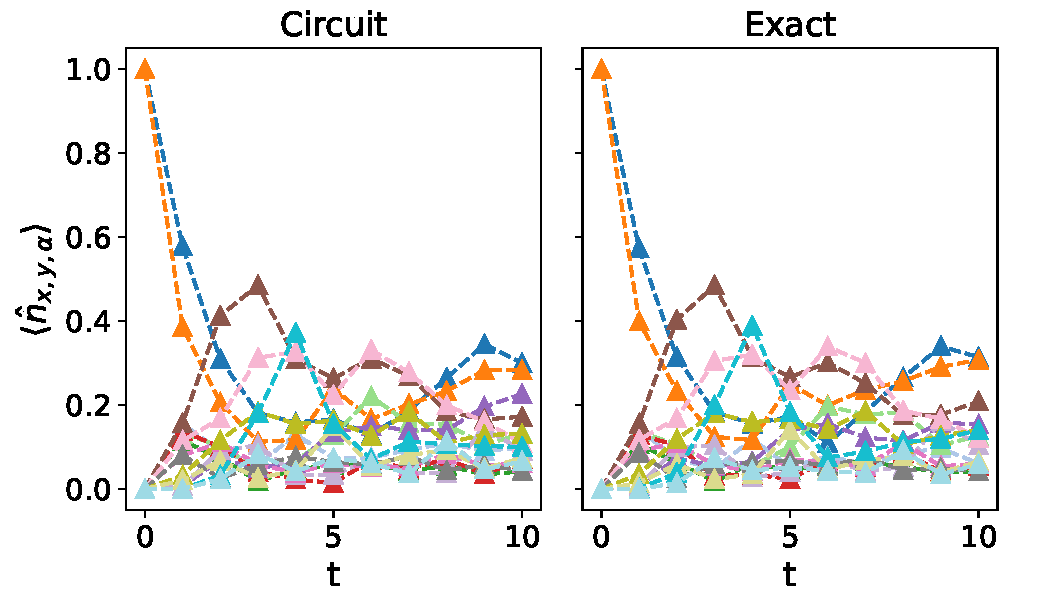
\includegraphics[width=\linewidth]{Picture/CircuitEvolve_ManyBody.pdf}
	% 		\caption{Single Excitation}
	% 		\label{fig:08}
	% 	\end{minipage}
	% 	\hfill
	% 	\begin{minipage}[b]{0.49\linewidth}
	% 		\centering
	% 		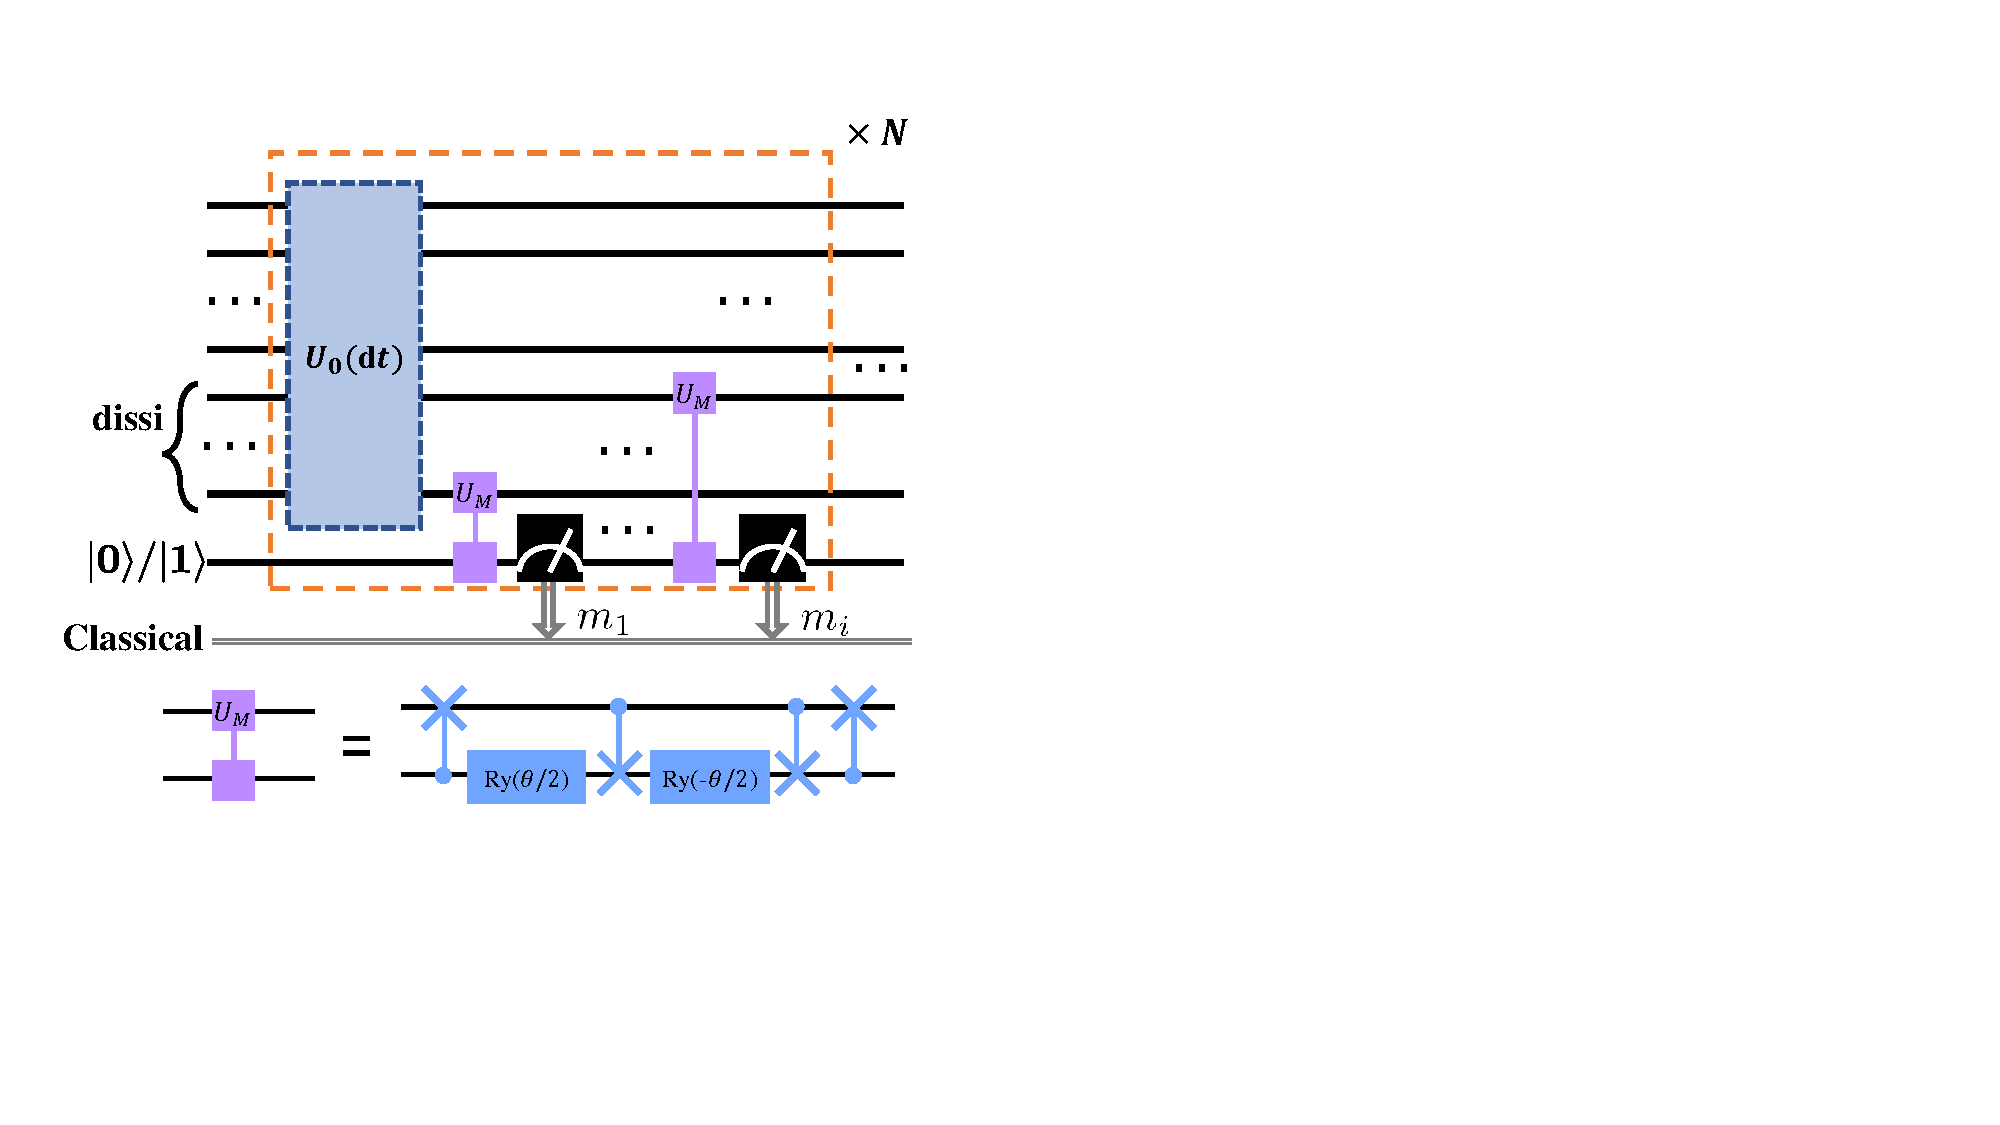
\includegraphics[width=\linewidth]{Picture/Circuit_Experiment.pdf}
	% 		\caption{Monitored quantum circuits.}
	% 		\label{fig:07}
	% 	\end{minipage}
	% \end{figure*}

	% \section{The localized states in larger system size~\label{sec:appendixE_comp}}
	% \begin{figure*}
	% 	\centering
	% 	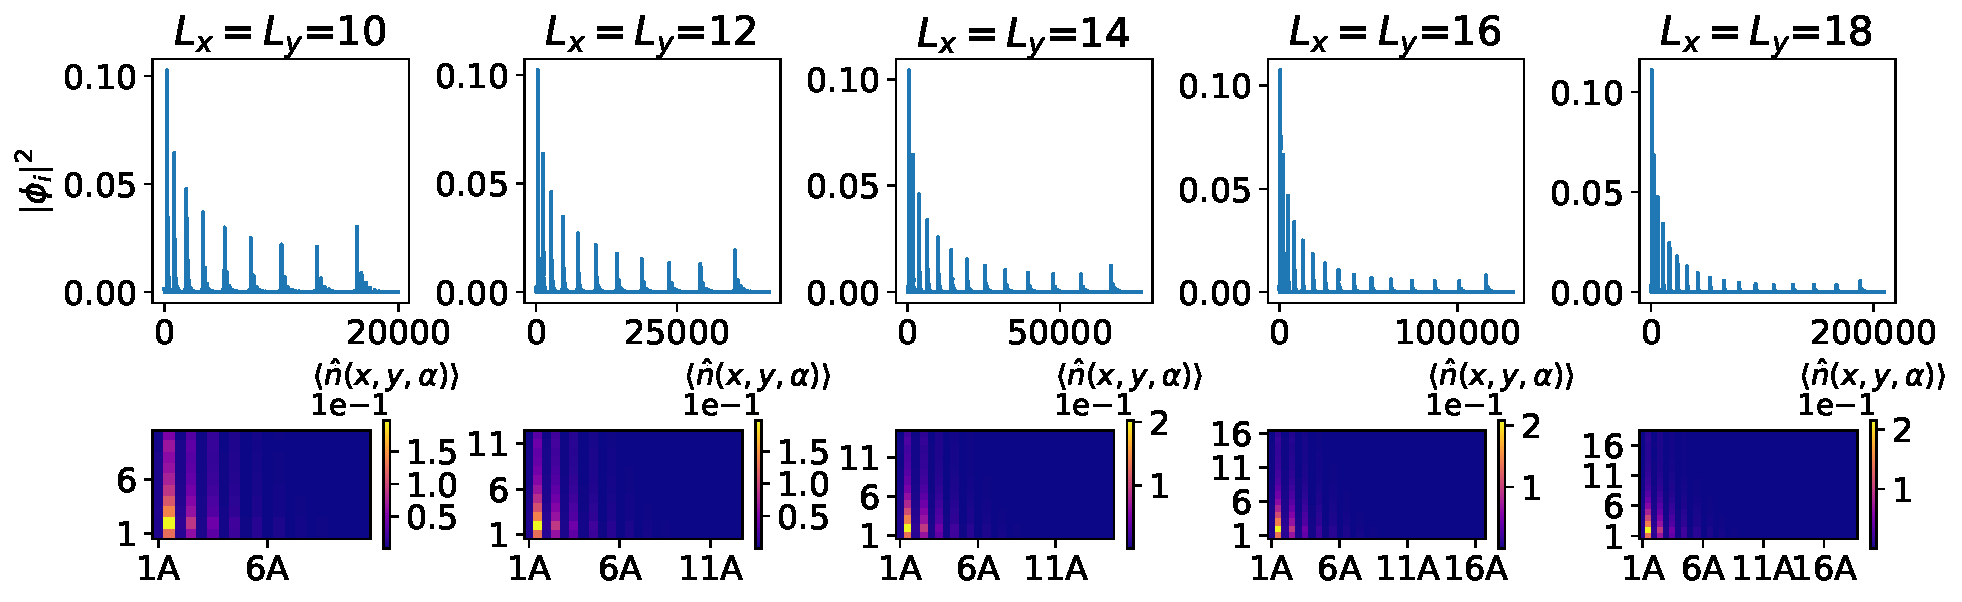
\includegraphics[width=1.\linewidth]{Picture/SI/LargeTwoExcitation.pdf}
	% 	\begin{overpic}[width=1.0\linewidth]{Picture/SI/LargeTwoExcitation_NotTopo.pdf}
	% 		\put(3,61){(a)}
	% 		\put(3,30){(b)}
	% 	\end{overpic}
	% 	\caption{%不同系统尺寸下的本征态和各个格点的粒子数算符平均值$\langle \hat{n}(x,y,\alpha) \rangle$。(a)通过Arnoldi方法计算系统尺寸为$L_x=L_y=[10,12,14,16,18]$的hybrid chiral skin correlated states.在位能为$u=-1.5$，当QWZ模型在不存在多体相互作用时，这个模型是拓扑绝缘体。
	% 	%(b)通过Arnoldi方法计算系统尺寸为$L_x=L_y=[10,12,14,16,18]$的non-Hermitian many-body induced localized states.在位能为$u=-2.1$，当QWZ模型在不存在多体相互作用时，这个模型是拓扑平庸的。
	% 	The probability distribution of eigenstates with the largest imaginary eigenvalue and average particle numbers $\langle \hat{n}(x,y,\alpha) \rangle$ of the eigenstate per lattice site for different system sizes.
	% 	(a) hybrid chiral skin correlated states, calculated with the Arnoldi method, for system sizes $L_x=L_y=[10,12,14,16,18]$. The onsite potential of the QWZ model is $u=-1.5$ and the QWZ model is a topological insulator.
	% 	(b) Non-Hermitian many-body induced localized states, calculated with the Arnoldi method, for system sizes $L_x=L_y=[10,12,14,16,18]$. 
	% 	The onsite potential of the QWZ model is $u=-2.1$ and the QWZ model is a topologically trivial.
	% 	}
	% 	\label{fig:14}
	% \end{figure*}
	% \begin{figure}[h]
	% 	\centering
	% 	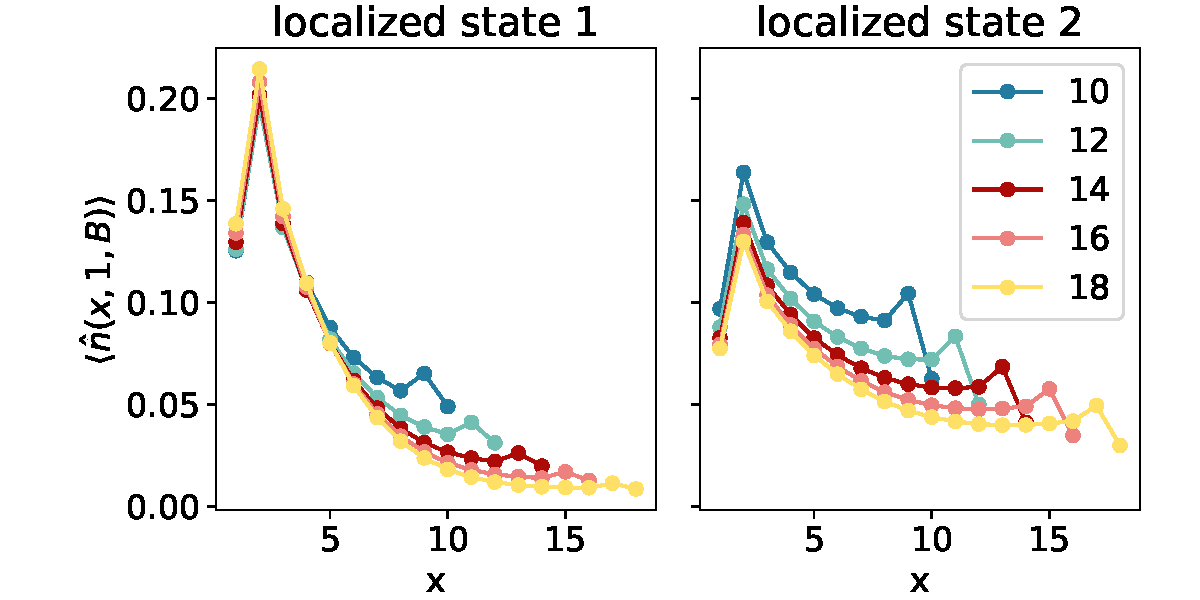
\includegraphics[width=1.\linewidth]{Picture/SI/SI_Comp1.pdf}
	% 	% 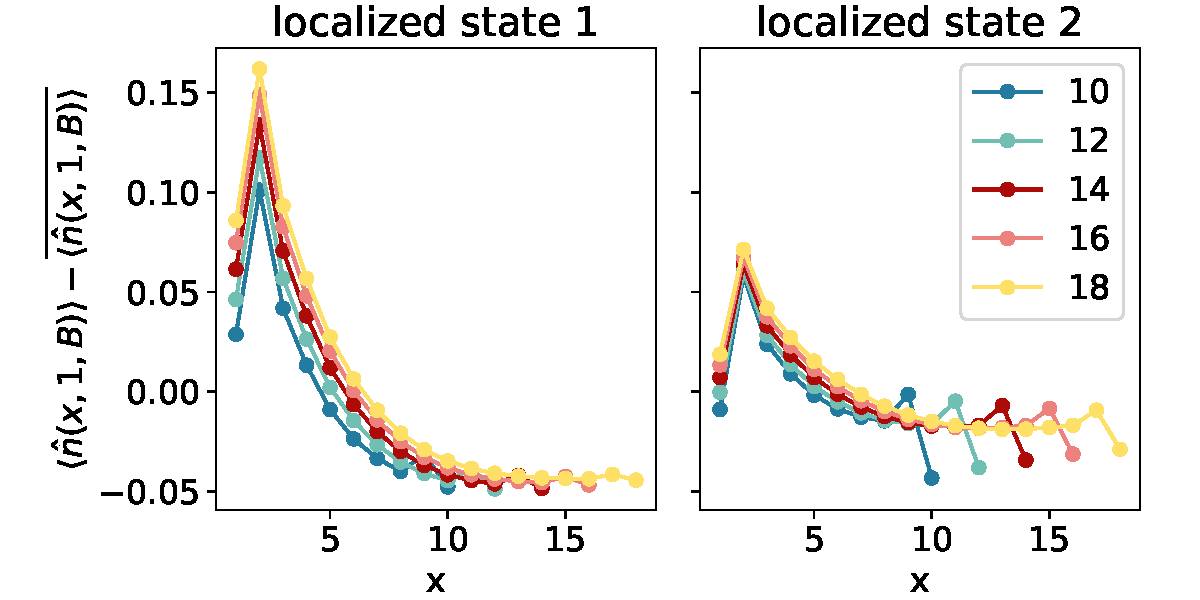
\includegraphics[width=1.\linewidth]{Picture/SI/SI_Comp2.pdf}
	% 	\begin{overpic}[width=1.0\linewidth]{Picture/SI/SI_Comp2.pdf}
	% 		\put(6,98){(a)}
	% 		\put(54,98){(b)}
	% 		% \put(7,54){(c)}
	% 		\put(6,48){(c)}
	% 		\put(54,48){(d)}
	% 	\end{overpic}
	% 	\caption{%不同$x$坐标，$y=1$的$B$子格点的粒子数算符平均值$\langle \hat{n}(x,1,B) \rangle$以及粒子数算符平均值与平均值的差$\langle \hat{n}(x,1,B) \rangle - \overline{\langle \hat{n}(x,1,B) \rangle}$。hybrid chiral skin correlated states，标记为localized state 1，的(a)粒子数算符平均值$\langle \hat{n}(x,1,B) \rangle$和(b)粒子数算符平均值和平均值的差$\langle \hat{n}(x,1,B) \rangle - \overline{\langle \hat{n}(x,1,B)\rangle}$。non-Hermitian many-body induced localized states，标记为localized state 2,的(a)粒子数算符平均值$\langle \hat{n}(x,1,B) \rangle$和(b)粒子数算符平均值和平均值的差$\langle \hat{n}(x,1,B) \rangle - \overline{\langle \hat{n}(x,1,B) \rangle}$。
	% 	Average particle number $\langle \hat{n}(x, 1, B) \rangle $ and the deviations from the average $\langle \hat{n}(x, 1, B) \rangle - \overline{\langle \hat{n}(x, 1, B) \rangle}$ for B sublattice at $y = 1$ boundary. 
	% 	(a) The average particle number and the deviations from the average of the hybrid chiral skin correlated states (localized state 1). The $x$-axis is the location of the unit cell in $x$ direction.
	% 	(b) The average particle number and the deviations from the average of non-Hermitian many-body induced localized states (localized state 2).  The $x$-axis is the location of the unit cell in $x$ direction.
	% 	}
	% 	\label{fig:15}
	% \end{figure}
	% In this section, we study the hybrid chiral skin correlated states and non-Hermitian many-body induced localized states in larger system sizes. 
	% % 我们研究具有chiral skin mode的模型($u=-1.5$)和不具有chiral skin mode的模型($u=-2.1$)。当$u=-1.5$时，QWZ模型是拓扑绝缘体，当$u=-2.1$时，QWZ模型是拓扑平庸的。当引入元胞间相互作用$\hat{H}_{\text{inter}}$的时候，具有chiral skin mode的模型会出现hybrid chiral skin correlated states, 不具有chiral skin mode的模型会出现non-Hermitian many-body induced localized states.
	% % 我们已经通过精确对角化的方法说明了，在系统尺寸到$L_x=L_y=9$时这样的localized states会存在。接下来我们采用Arnoldi方法说明在更大的系统尺寸下，本征值虚部最大的本征态仍然存在上述局域量子态。
	% % hybrid chiral skin correlated states 在更大系统尺寸的本征态以及该本征态在各个格点的粒子数平均值如Fig.~\ref{fig:14}(a)，non-Hermitian many-body induced localized在更大系统尺寸的本征态以及该本征态在各个格点的粒子数平均值如Fig.~\ref{fig:14}(b)所示。从Fig.~\ref{fig:14}中可以发现在更大系统尺寸下，局域量子态仍然存在，同时hybrid chiral skin correlated states更加局域。
	% We investigate the QWZ models with chiral skin modes ($u = -1.5$) and the QWZ models without chiral skin mode ($u = -2.1$). The QWZ models with onsite energy $u=-1.5$ are topological insulators, and the QWZ models with onsite energy $u = -2.1$ are trivial insulator. When inter-cell interactions $\hat{H}_{\text{inter}}$ are introduced, the model with chiral skin modes exhibits hybrid chiral skin correlated states, while the model without chiral skin modes exhibits non-Hermitian many-body induced localized states.
	% We have shown that such localized states exist for system sizes up to $L_x = L_y = 9$ with exact diagonalization method. To explore the localization in larger systems, we employ the Arnoldi method to compute the eigenstate with the largest imaginary eigenvalue. 
	% We find that this eigenstate exhibits localization.
	% The probability distribution of eigenstate and the average particle number of eigenstate for the hybrid chiral skin correlated states in larger systems are shown in Fig.\ref{fig:14} (a). 
	% The probability distribution of eigenstate and the average particle number of eigenstate for non-Hermitian many-body induced localized states are shown in Fig.\ref{fig:14} (b). The results in Fig.~\ref{fig:14} show these localized states still exist even in larger systems. Moreover, the hybrid chiral skin correlated states are more localized.

	% % 我们同时研究在不同系统尺度下，hybrid chiral skin correlated states(labeled as localized state 1)和non-Hermitian many-body induced localized states(labeled as localized state 2)沿着$x$方向，$y$坐标为$y=1$的B晶格的粒子数平均值$\langle \hat{n}(x,y,\alpha) \rangle$以及粒子数平均值与平均值的差$\langle \hat{n}(x,y,\alpha) \rangle - \overline{\langle \hat{n}(x,y,\alpha) \rangle}$。
	% % 结果显示，localized state 1的峰值大小不随着系统尺寸的增加而减小，而localized state 2的峰值大小会随着系统尺寸的增加而减小，如Fig.~\ref{fig:15}所示，Fig.~\ref{fig:15}(a)中的现象比Fig.~\ref{fig:15}(b)更具有局域性特征。
	% % 此外，从Fig.~\ref{fig:15}(c)和(d)中可以看出，粒子数算符平均值和平均值的差的峰值在localized state 1中随系统尺寸的增加而增加，而localized state 2中不随系统尺寸的变化而变化。
	% % 这是因为hybrid chiral skin correlated states是多体相互作用使得本来局域在corner上的chiral skin mode在格点上由于能级差进一步局域化。而non-Hermitian many-body induced localized states仅是由于多体相互作用和非厄米导致的，因此并不如hybrid chiral skin correlated states局域化。

	% We further investigate the behavior of hybrid chiral skin correlated states (labeled as localized state 1) and non-Hermitian many-body induced localized states (labeled as localized state 2) at different system sizes. Specifically, we study the average particle number $\langle \hat{n}(x, y, \alpha) \rangle$ and the deviation from average $\langle \hat{n}(x, y, \alpha) \rangle - \overline{\langle \hat{n}(x, y, \alpha) \rangle}$ along the $x$-direction for the $B$ sublattice at $y = 1$ boundary.
	% As shown in Fig.~\ref{fig:15}, the peak amplitude of localized state 1 does not decrease as the system size increases, whereas the peak amplitude of localized state 2 decreases as the system size increases. This indicates that the behavior shown in Fig.\ref{fig:15} (a) is more localized than that in Fig.~\ref{fig:15} (b).
	% Moreover, Fig.~\ref{fig:15} (c) and Fig.~\ref{fig:15} (d) reveal that the peak values of the deviation from average increases as system size increases for localized state 1, but remain nearly constant for localized state 2.
	% hybrid chiral skin correlated states originate from many-body interactions that enhance the localization of topological corner states. 
	% The energy splitting induced by many-body interactions further localizes these modes along both directions and confines them to the $B$ sublattice.
	% In contrast, non-Hermitian many-body induced localized states arise from the combined effects of non-Hermiticity and many-body interactions. These states do not dependent on the presence of localized topological corner state, called chiral skin mode, and therefore exhibit comparatively weaker localization.

	% \section{The spectrum in the three-excitation subspace for system size $L_x=L_y=4$~\label{sec:AddtionalSpectrum3}}

	% 	Fig.~\ref{fig:17} (a1) shows the energy spectrum in the three-excitation subspace for the non-Hermitian many-body Hamiltonians with a system size of $L_x=L_y=4$. In Fig.~\ref{fig:17} (a2), the probability distribution of the eigenstate with the largest imaginary eigenvalue (orange cross in Fig.~\ref{fig:17}) is shown. This eigenstate typically dominates the long-time dynamics governed by non-Hermitian many-body Hamiltonians.
	% 	Fig.~\ref{fig:17} (a3) shows the average particle number $\langle \hat{n}(x,y,\alpha) \rangle$ at each lattice site for the eigenstate. 
	% 	%The hybrid chiral skin correlated states in Fig.~\ref{fig:17} (a3) is not clear, because the calculation is restriction to system size $L_x=L_y=4$.
	% 	Although signatures of hybrid chiral skin effects are expected in this eigenstate, these features are not clearly resolved due to the constraints imposed by the small system size ($L_x = L_y = 4$).

	% %We show the spectrum and eigenstates in three-excitation subspace for system size $L_x=L_y=4$ in Fig.~\ref{fig:17} (a1-a3). The hybrid chiral skin correlated states is not clear, because the calculation is restriction to system size $L_x=L_y=4$.
	% \begin{figure}[h]
	% 	\centering
	% 	\begin{overpic}[width=1.0\linewidth]{Picture/SI/SI_EvolveSpectrum3.pdf}
	% 		\put(5,83){(a1)}
	% 		\put(54,83){(a2)}
	% 		\put(5,36){(a3)}
	% 	\end{overpic}
	% 	\caption{
	% 	The spectrum and eigenstate in the three-excitation subspace. The non-Hermitian gain ($\gamma=0.2$) is applied to unit cells at the $y=1$ boundary, and the many-body interaction is $\hat{H}_{\text{inter}}$. The system size for (b1-b3) is $L_x=L_y=5$. The onsite potential is $u=-1.5$.
	% 	(a1) The spectrum of a non-Hermitian many-body Hamiltonian.
	% 	(a2) The probability distribution of the eigenstate of a non-Hermitian many-body Hamiltonian. 
	% 	(a3) The average particle number per lattice site for the eigenstate.
	% 	}
	% 	\label{fig:17}
	% \end{figure} %label from y=1 and x=1?


	\section{Three-excitation Subspace~\label{sec:three_excitation}}
	\begin{figure*}[htbp]
		% \begin{minipage}[b]{0.55\textwidth}
		% 	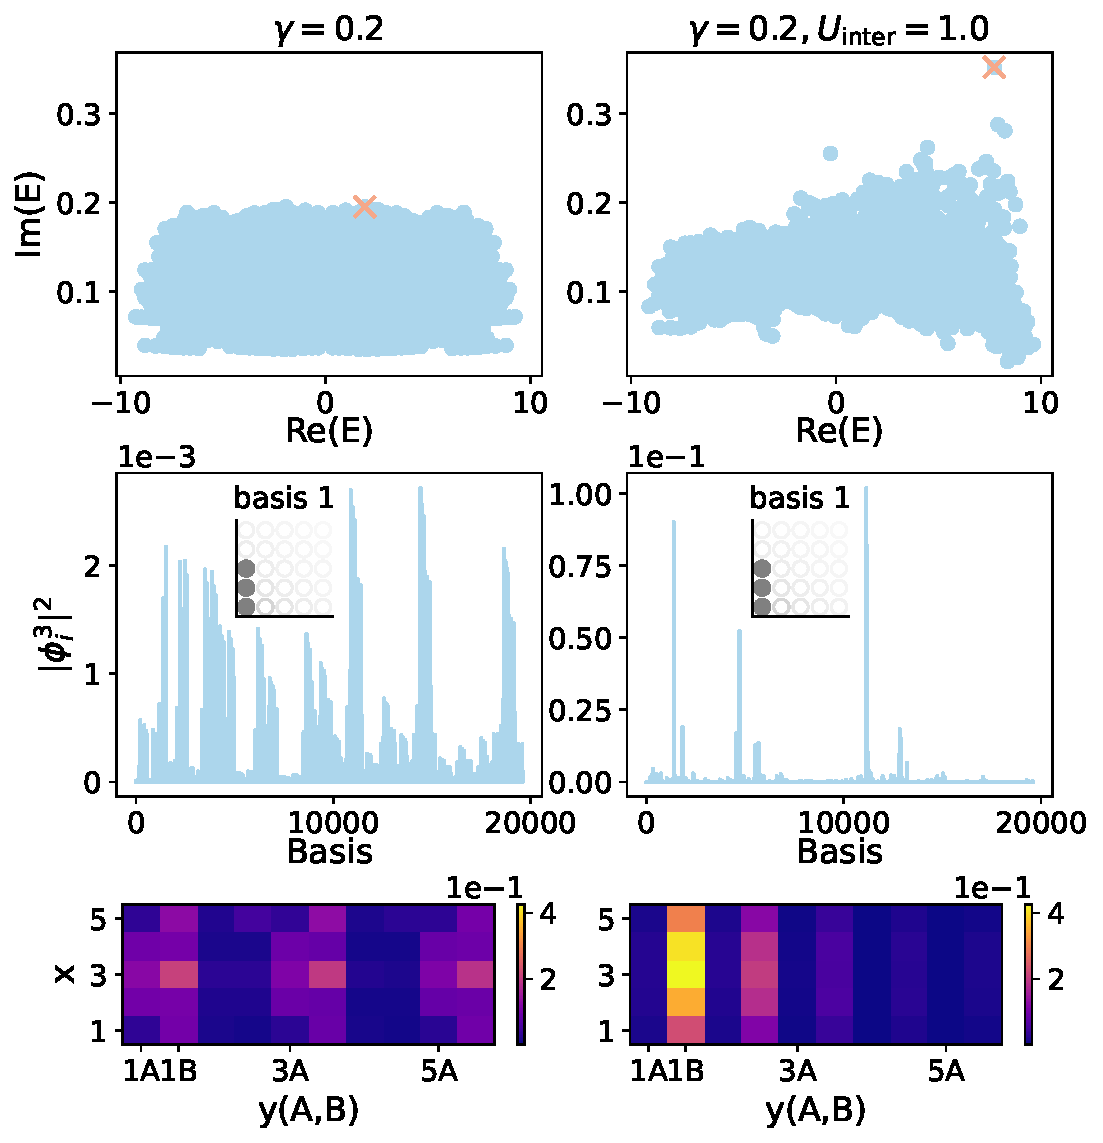
\includegraphics[width=\textwidth]{Picture/ThreeExcitationSpectrum.pdf}
		% 	% \caption{图片3说明}
		% 	% \label{fig:img3}
		% \end{minipage}
		% \hfill
		% % \begin{minipage}[b]{0.48\textwidth}
		% % 	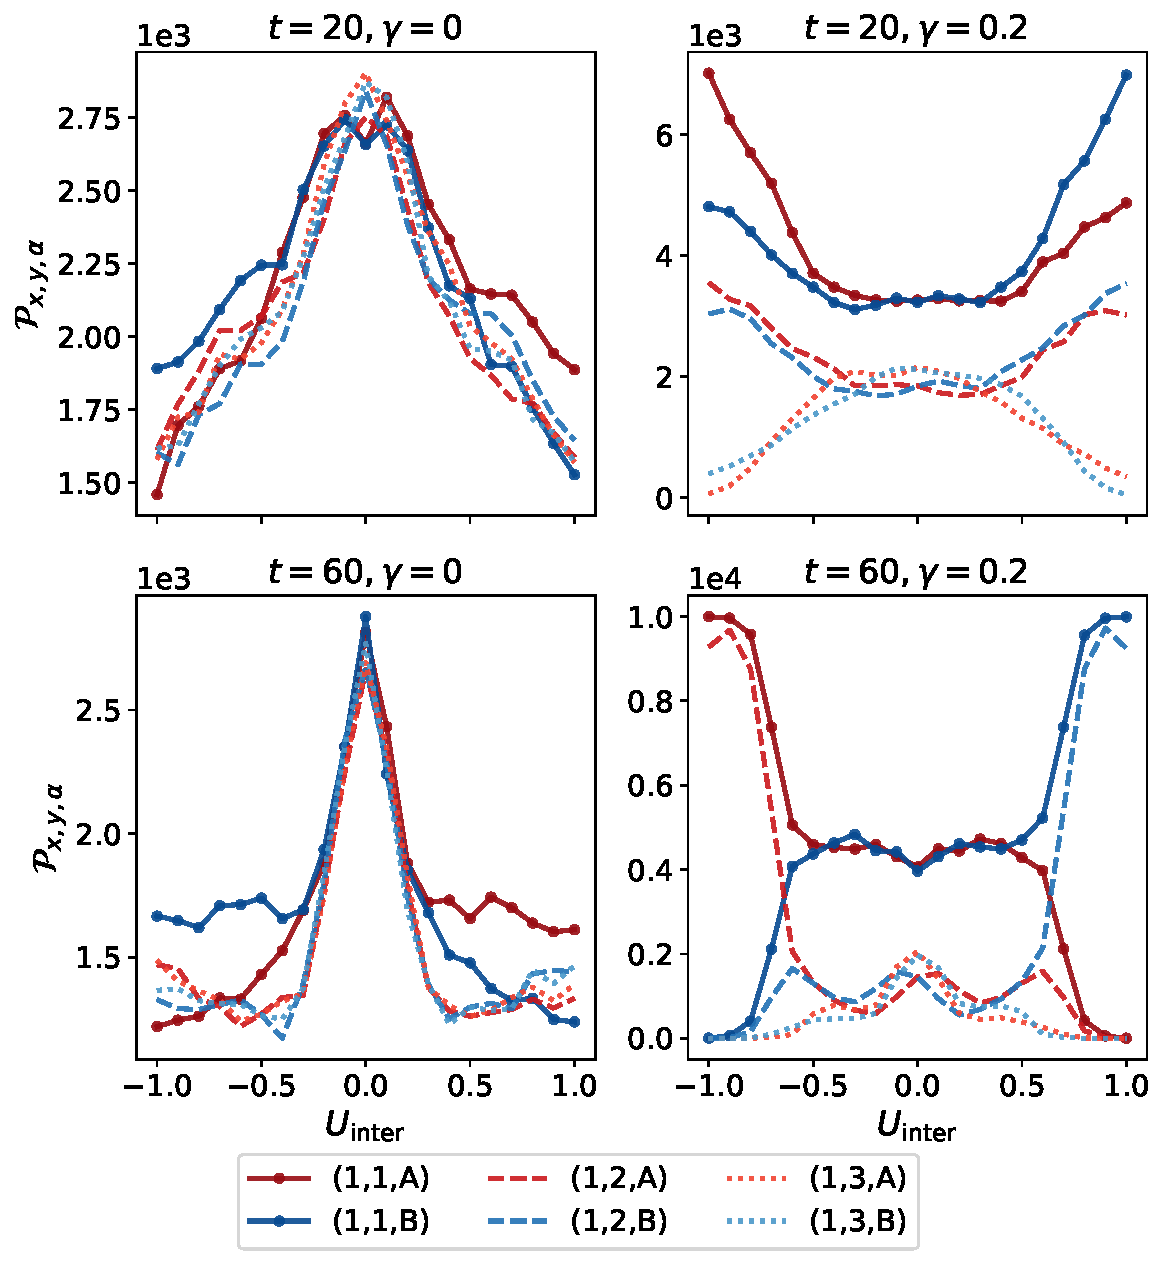
\includegraphics[width=\textwidth]{Picture/ThreeExcitation_Popu_Interaction.pdf}
		% % 	% \caption{图片4说明}
		% % 	% \label{fig:img4}
		% % \end{minipage}
		% \begin{minipage}[b]{0.43\textwidth}
		% 	% 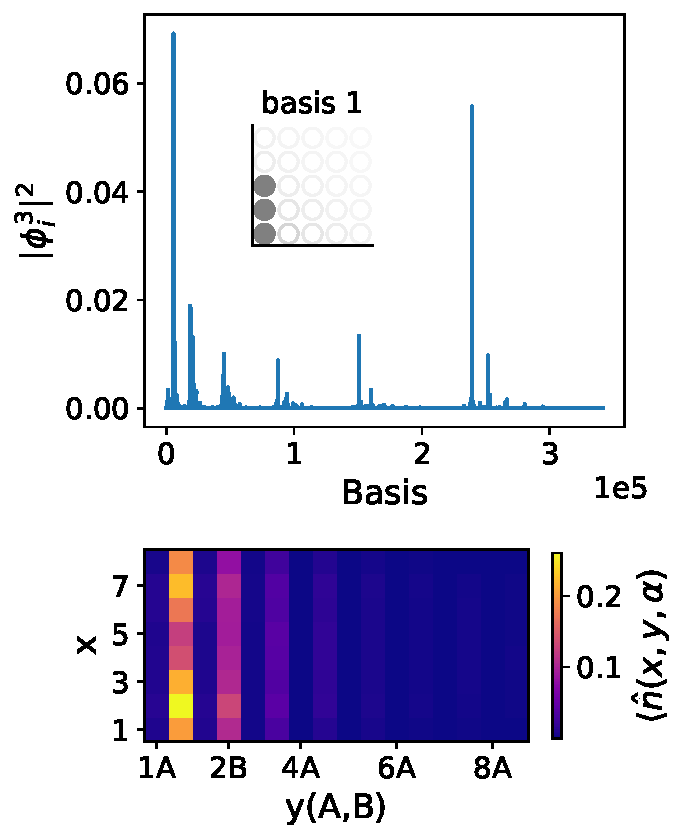
\includegraphics[width=1.\linewidth]{Picture/SI/SI_ThreeExcitationSize8.pdf}
		% 	\begin{overpic}[width=1.\linewidth]{Picture/SI/SI_ThreeExcitationSize8.pdf}
		% 		\put(-103,105){(a)}
		% 		% \put(7,54){(c)}
		% 		\put(0,105){(b)}
		% 		% \put(49,54){(d)}
		% 	\end{overpic}
		% 	% \caption{图片4说明}
		% 	% \label{fig:img4}
		% \end{minipage}
		\begin{minipage}[b]{0.665\textwidth}
			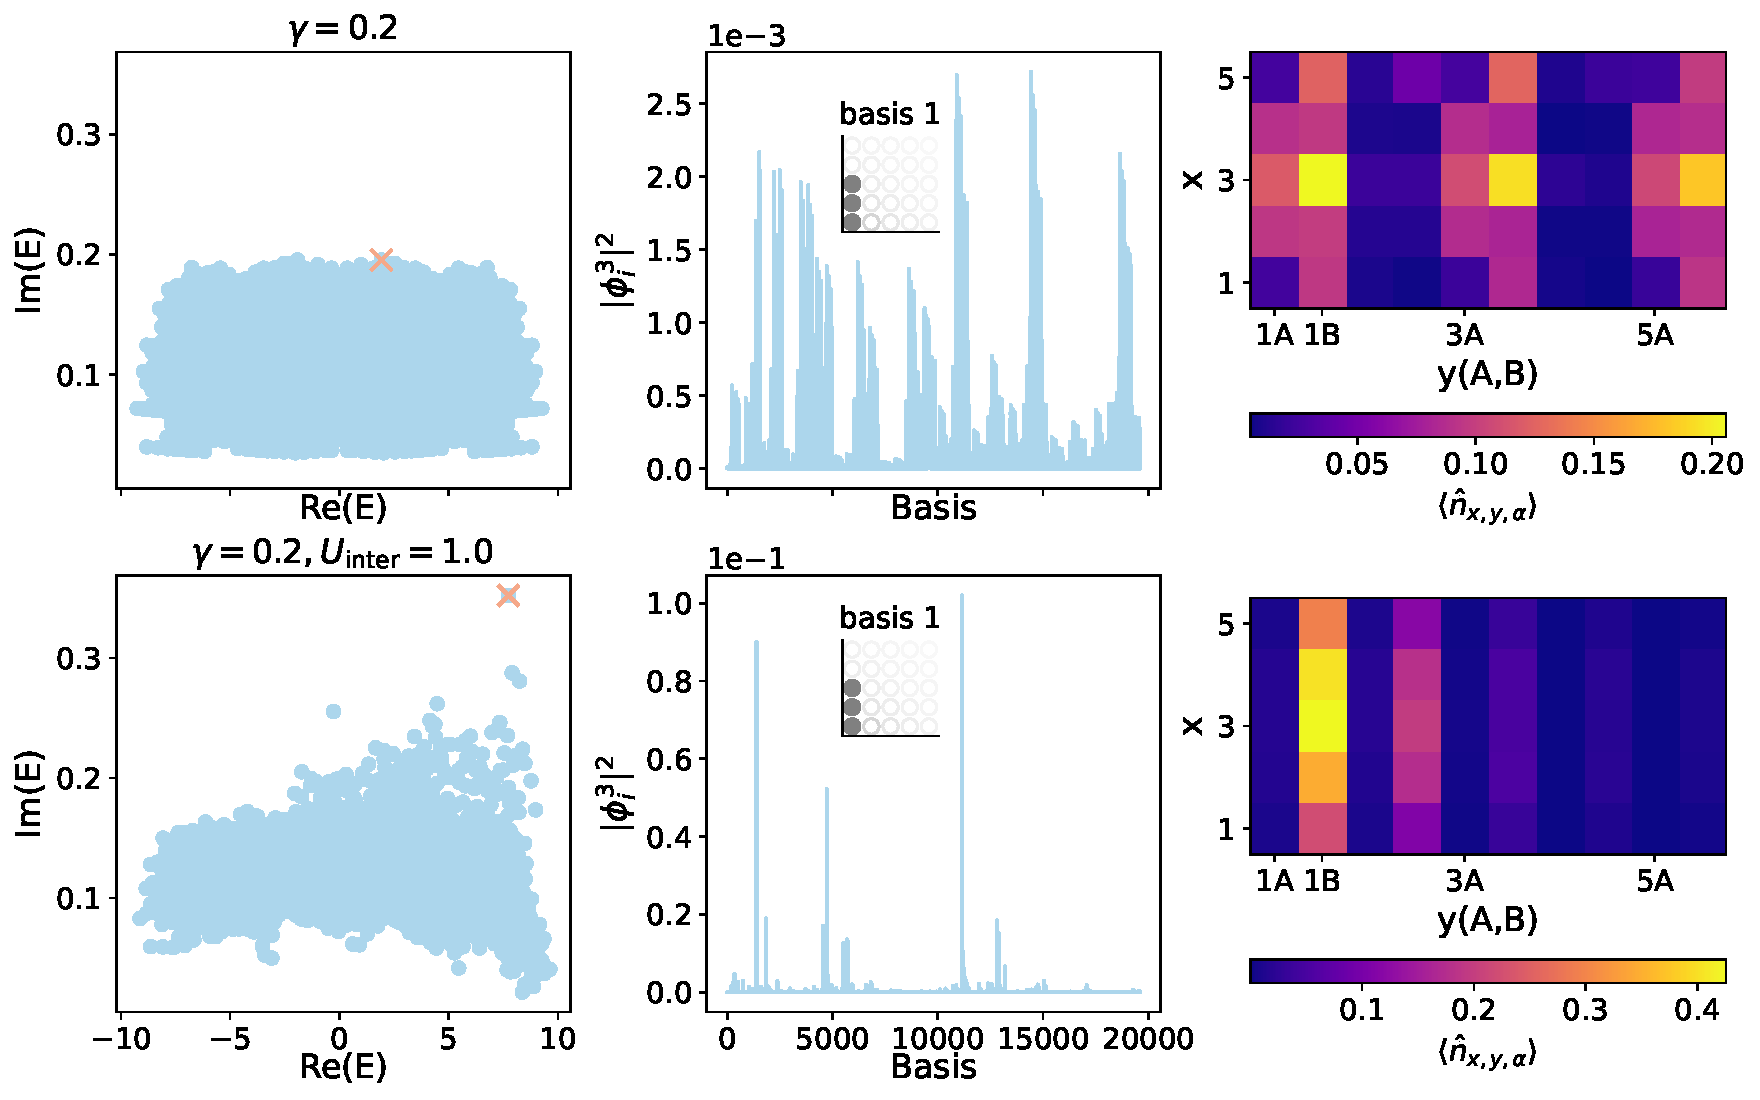
\includegraphics[width=\textwidth]{Picture/ThreeExcitationSpectrum2.pdf}
			% \caption{图片3说明}
			% \label{fig:img3}
		\end{minipage}
		\hfill
		\begin{minipage}[b]{0.325\textwidth}
			% 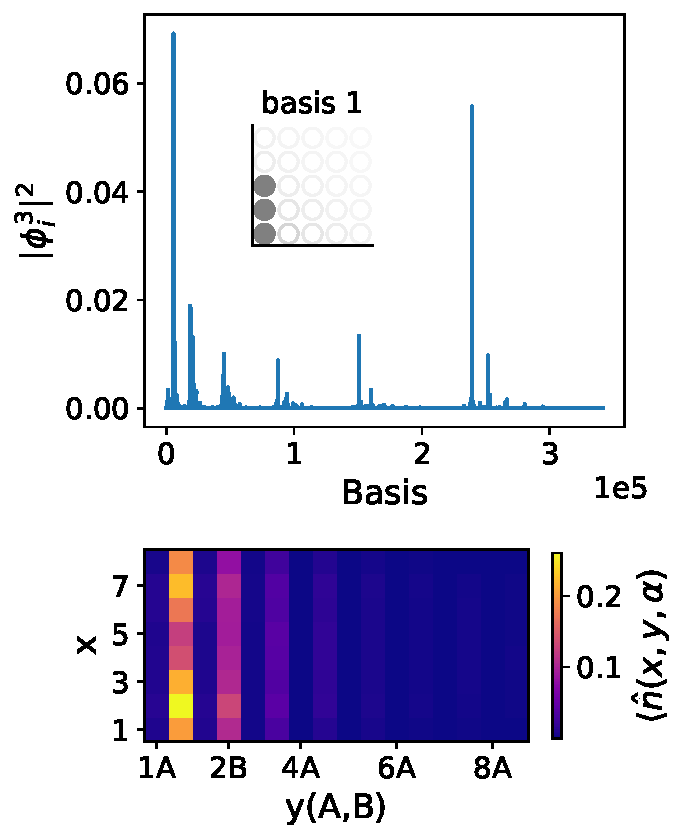
\includegraphics[width=1.\linewidth]{Picture/SI/SI_ThreeExcitationSize8.pdf}
			\begin{overpic}[width=1.\linewidth]{Picture/SI/SI_ThreeExcitationSize8.pdf}
				\put(-165,102){(a1)}
				\put(-165,52){(b1)}
				\put(-112,102){(a2)}
				\put(-112,52){(b2)}
				\put(-58,102){(a3)}
				\put(-58,52){(b3)}
				% \put(7,54){(c)}
				\put(10,102){(c)}
				% \put(49,54){(d)}
			\end{overpic}
			% \caption{图片4说明}
			% \label{fig:img4}
		\end{minipage}

		\caption{%(a) 三激发子空间中能谱和本征态对比。在不存在相互作用和存在相互作用时的能谱，本征态模方和本征态各个格点的粒子数算符平均值，其复能量在能谱中用橘色十字表示。系统尺寸为$L_x=L_y=5$，在位能为$u=-1.5$。
		%(b) 在系统尺寸为$L_x=L_y=8$时具有最大虚本征值的本征态，以及该本征态在各个格点的粒子数平均值$\langle \hat{n}(x,y,\alpha) \rangle$，该态就是在三激发子空间的hybrid chiral skin correlated states.
		%(c) 在时间$t=20$和$t=60$时，相互作用为$\hat{H}_{\text{inter}}$,不同相互作用强度下的$\mathcal{P}_{x,y,\alpha}$。增益作用于$y=1$元胞。系统尺寸为$L_x=L_y=7$，在位能为$u=-1.5$。选取的随机初始量子态数目为$N_{\text{samp}}=10^4$。
		%(d) 在存在相互作用$\hat{H}_{\text{inter}}$的非厄米多体哈密顿量的双激发子空间部分量子态示意图。每个蓝色圆球表示一个元胞，前三个元胞存在非厄米增益，元胞上的蓝色向下箭头表示在该元胞的$A$子格点有一个粒子，红色向上箭头表示在该元胞的$B$子格点有一个粒子，黑色箭头表示允许的量子跃迁。总共存在三个粒子。蓝色波浪箭头表示非厄米pumping，它表示在经历时间演化之后粒子会被pump到这些量子态，蓝色波浪线箭头的数目代表pump的强度。$U$表示由于相互作用导致出现的能级差。
		The spectrum, the probability distribution of eigenstate and eigenstate's average particle number $\langle \hat{n}(x,y,\alpha) \rangle$ of non-Hermitian Hamiltonian. The comparisons of them (a) without interaction and (b) with interaction $\hat{H}_{\text{inter}}$ in three-excitation subspace. 
		The complex energy of eigenstate is marked by a orange cross in the spectrum. The system size is $L_x = L_y = 5$, and the onsite potential is $u = -1.5$.
		(c) The probability distribution and average particle number of eigenstate with largest imaginary eigenvalue atsystem size $L_x=L_y=8$. This state corresponds to the hybrid chiral skin correlated states in the three-excitation subspace.
		}
		\label{fig:03}
	\end{figure*}

	% \begin{figure*}
	% 	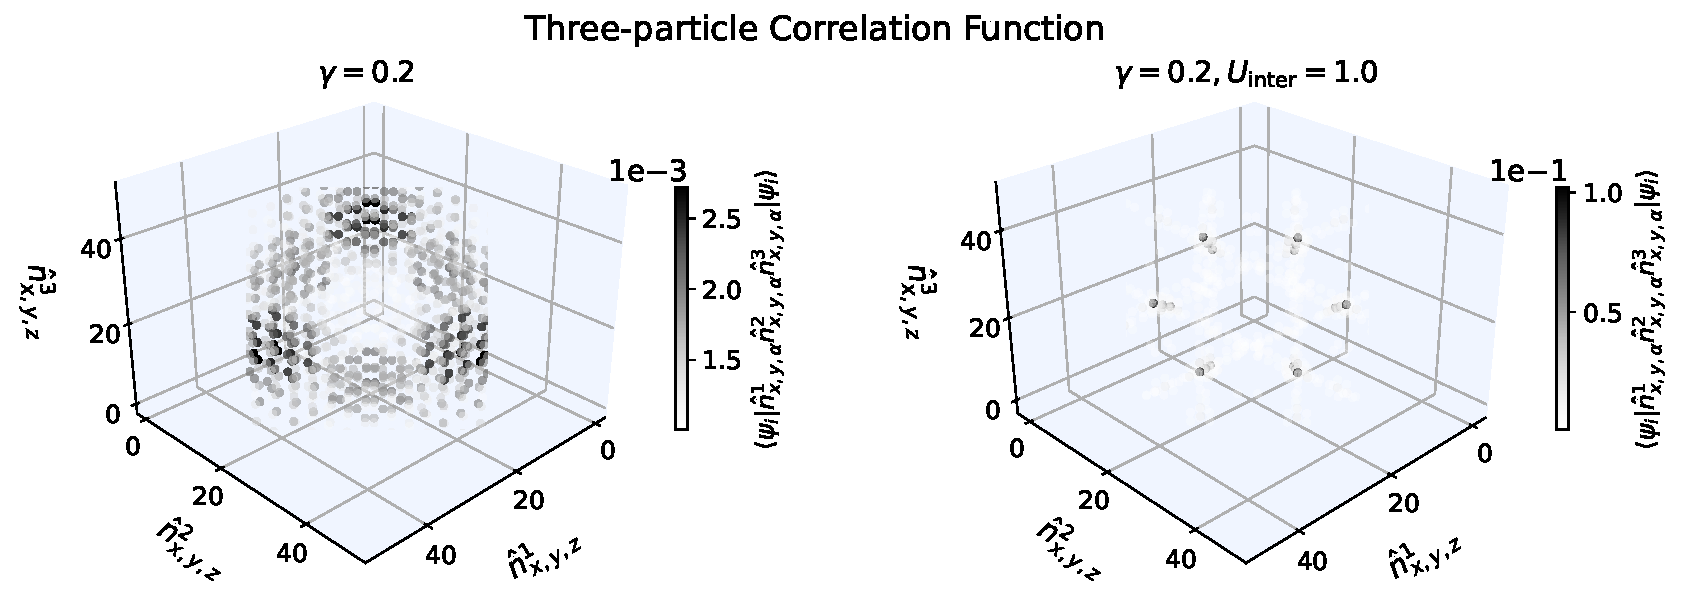
\includegraphics[width=0.95\linewidth]{Picture/CorrelationMap_3P.pdf}
	% 	% \caption{图片4说明}
	% 	% \label{fig:img4}
	% 	\caption{The three-particle correlation function $\langle \phi_i \vert \hat{n}^1_{x,y,\alpha} \hat{n}^2_{x,y,\alpha} \hat{n}^3_{x,y,\alpha} \vert \phi_i \rangle$ bwteen three particles of the eigenstate with the largest imaginary eigenvalue under different non-Hermitian Hamiltonians. The system size is $L_x=L_y=5$ and the onsite potential is $u=-1.5$. The non-Hermitian gain is applied to $y=1$ boundary.}
	% 	\label{fig:03_Supple}
	% \end{figure*}
	\begin{figure*}
		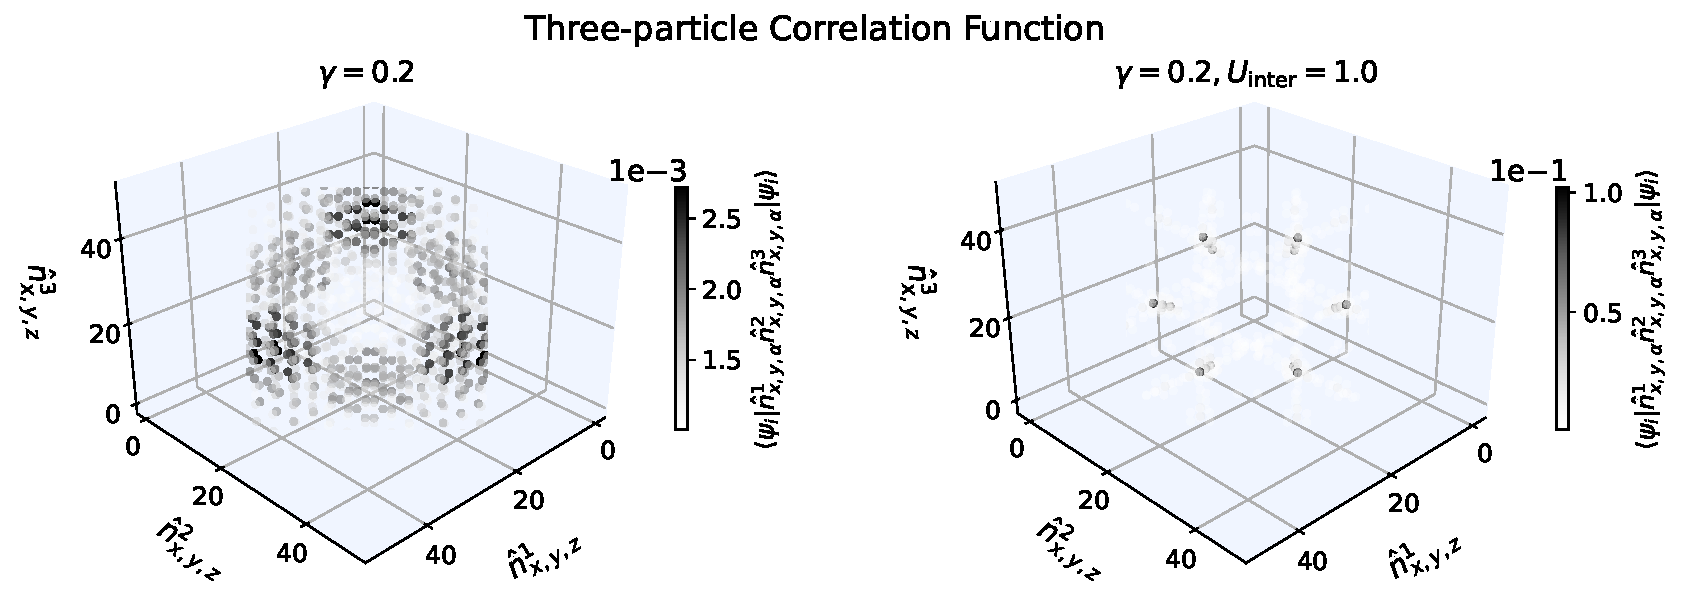
\includegraphics[width=0.98\linewidth]{Picture/CorrelationMap_3P.pdf}
		\begin{minipage}[b]{1.\textwidth}
			% 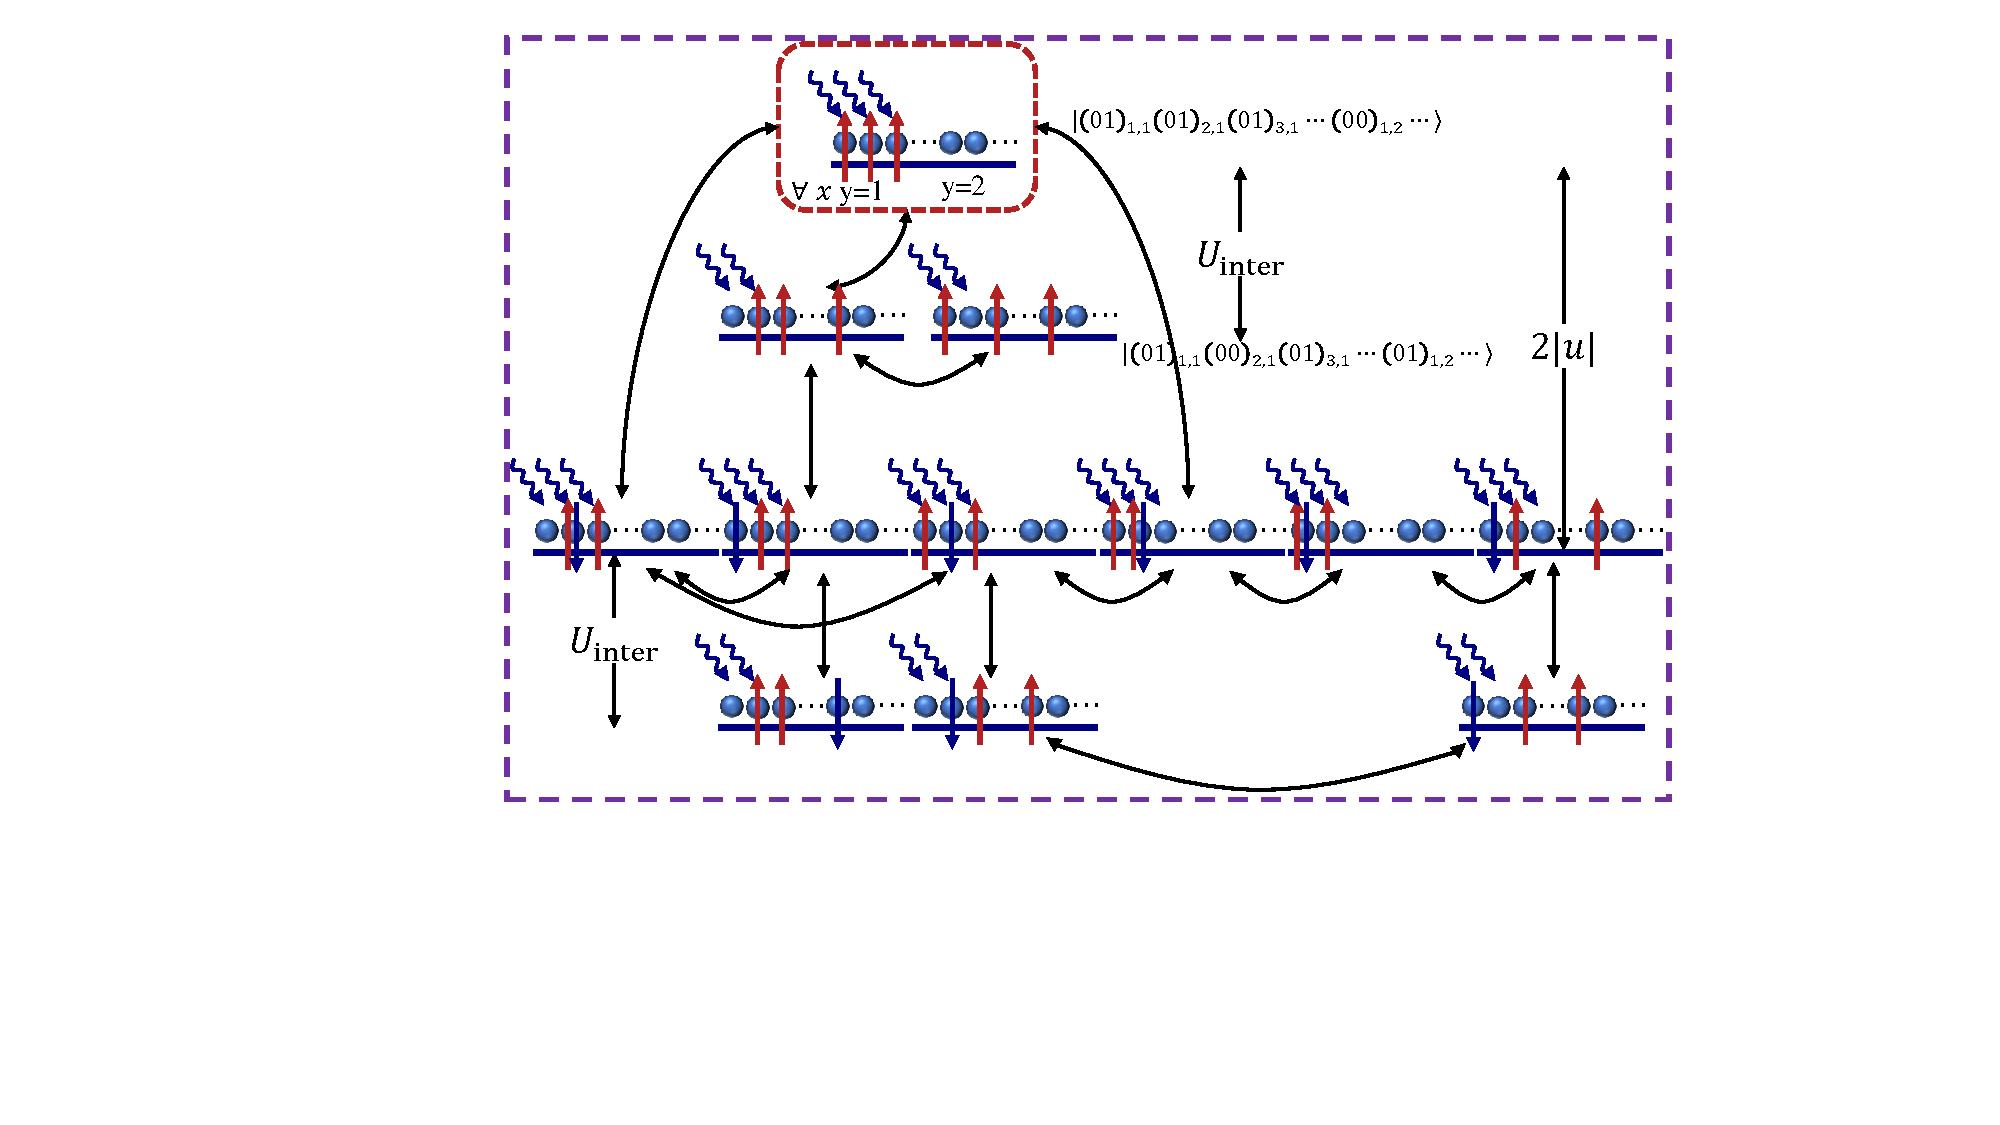
\includegraphics[width=\textwidth]{Picture/3D_Mechanism_inter.pdf}
			% 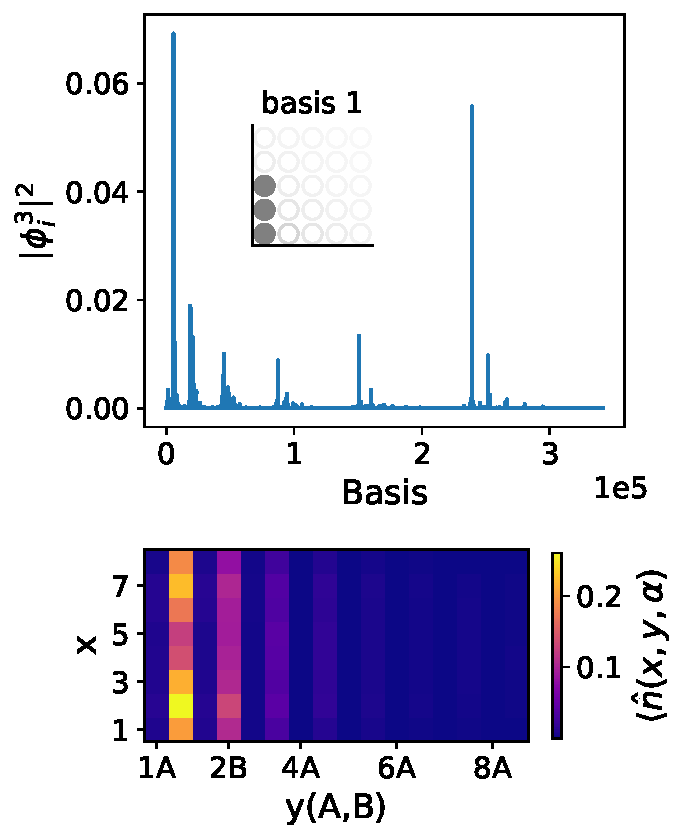
\includegraphics[width=0.29\linewidth]{Picture/SI/SI_ThreeExcitationSize8.pdf}
			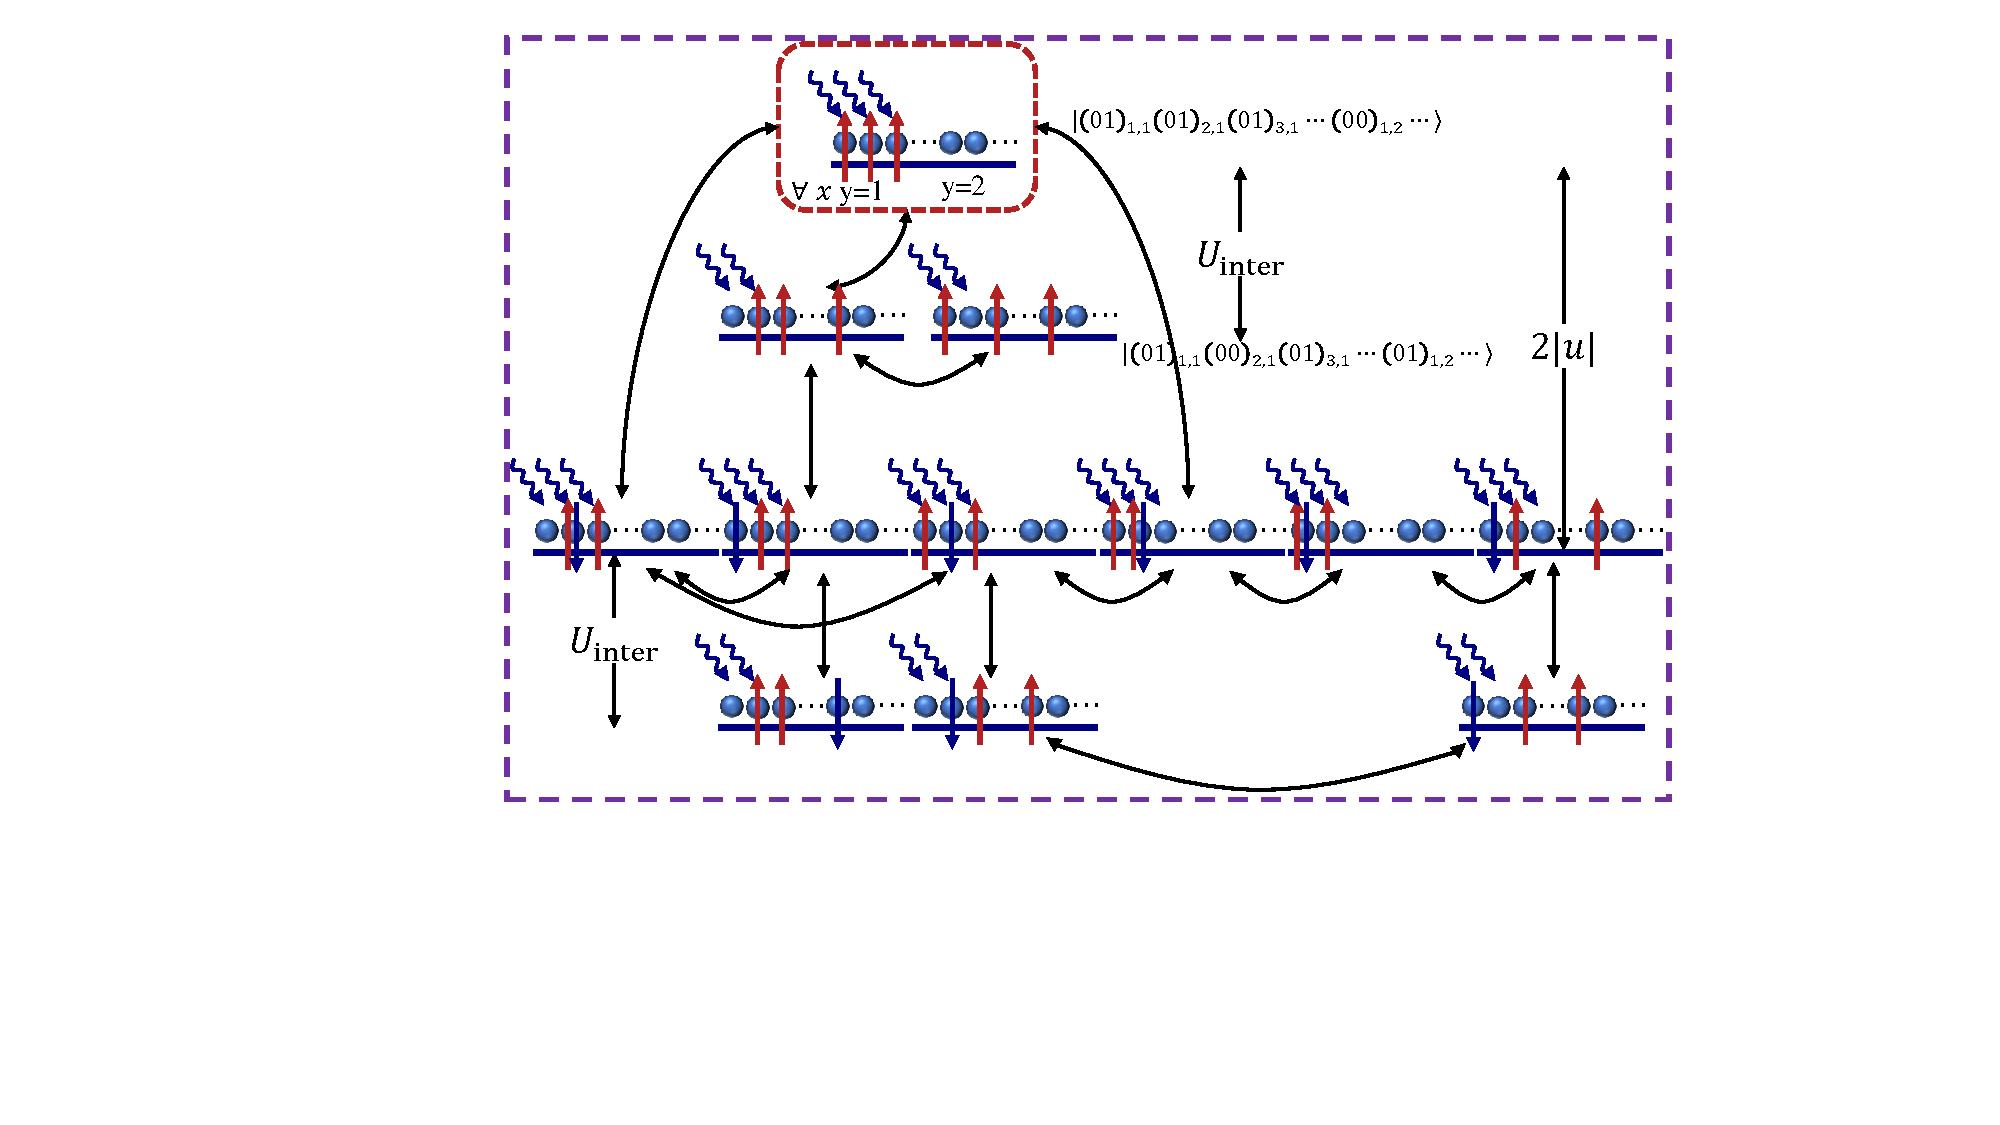
\includegraphics[width=0.6\linewidth]{Picture/3D_Mechanism_inter.pdf}
			\begin{overpic}[width=0.38\linewidth]{Picture/ThreeExcitation_Popu_Interaction.pdf}
				\put(-150,175){(a)}
				\put(-150,98){(b)}
				\put(0,98){(c)}
				% \put(49,54){(d)}
			\end{overpic}
			% \caption{图片1说明}
			% \label{fig:img1}
		\end{minipage}
		% \caption{图片4说明}
		% \label{fig:img4}
		\caption{(a) The three-particle correlation function $\langle \phi_i \vert \hat{n}^1_{x,y,\alpha} \hat{n}^2_{x,y,\alpha} \hat{n}^3_{x,y,\alpha} \vert \phi_i \rangle$ bwteen three particles of the eigenstate with the largest imaginary eigenvalue under different non-Hermitian Hamiltonians. The system size is $L_x=L_y=5$ and the onsite potential is $u=-1.5$. The non-Hermitian gain is applied to $y=1$ boundary.
		(b) A schematic diagram of quantum states in the three-excitation subspace of the interacting non-Hermitian many-body Hamiltonian. 
		Blue spheres: unit cells; blue downward arrows (red upward arrows): particles at $A$ ($B$) sublattice; black arrows: allowed transitions; blue wavy arrows: non-Hermitian pumping (arrow number indicates strength). The gain is applied to the first three unit cells ($y=1$ boundary). 
		The energy splitting induced by interactions is denoted by $U_{\text{inter}}$.
		(c) The parameters $\mathcal{P}_{x,y,\alpha}$ at time $t=20$ and $t=60$ under different interaction strengths. Gain is applied to the $y=1$ unit cell. The system size is $L_x=L_y=7$, and the onsite potential is $u=-1.5$. The number of randomly selected initial quantum states is $N_{\text{samp}}=10^4$. 
		}
		\label{fig:03_Supple}
	\end{figure*}

	% 上述分析和计算可以拓展到更多粒子激发的子空间。我们考虑了一个大小为$L_x=L_y=5$的二维晶格。为了计算方便，由于粒子数算符和哈密顿量的对易性，我们考虑三激发的子空间。在Fig.~\ref{fig:03} (a)中，我们展示了在三激发子空间中非厄米哈密顿量和非厄米多体哈密顿量的复能谱、最大虚本征值的本征态，其复能量在能谱中用橘色十字表示，以及该态的每个格点上的粒子数算符的平均值。本征态的横坐标表示不同基矢，每个基矢均对应于一个三激发量子态（相关构型可参见Fig.~\ref{fig；03}(a)中的插图示意）。
	% 结果显示，非厄米哈密顿量的能谱由于anti-$\mathcal{PT}$对称性，表现出关于能谱虚轴的对称性，然而，当引入多体相互作用时，该对称性不再成立。
	% 与之前的分析一致，随着多体相互作用的引入，本征态以及粒子数算符的平均值都表现出局域化现象。需要注意的是，由于三激发空间的计算仅限于$L_x=L_y=5$，Fig.~\ref{fig:03} (a)中非厄米哈密顿量中的本征态并非三粒子的chiral skin mode。
	% %对三激发情况下，最大虚本征值的本征态对应的量子态仍然是hybrid chiral skin correlated states,
	% 但是此时非厄米多体哈密顿量的最大虚本征值所对应的本征态仍呈现局域化量子态特征。
	% 通过对系统尺寸为$L_x=L_y=8$的三激发子空间中非厄米多体哈密顿量进行Arnoldi数值对角化计算，我们发现hybrid chiral skin correlated states在更高激发子空间仍然存在(Fig~\ref{fig:03}(c))。
	% 因此，在更高粒子激发的子空间内，非厄米多体哈密顿量仍然表现出hybrid chiral skin correlated states。

	% Due to the commutation between the number operator and the Hamiltonian, excitation subspaces are decoupled. 
	So far, we have focused on the two-excitation subspace. However, the interplay between topological states and many-body interactions persists even in the higher-excitation subspace. The hybrid chiral skin correlated states can also be found. 
	We consider a two-dimensional lattice with size $L_x = L_y = 5$ for our investigation. For computational convenience, we focus on the three-particle excitation subspace due to the commutation of particle number operator and Hamiltonian. 
	Figs.~\ref{fig:03} (a1) and (b1) show the energy spectrum
	%, the eigenstate with the largest imaginary eigenvalue, and the average particle number of this eigenstate 
	for the non-Hermitian Hamiltonian with or without many-body interactions. 
	% The complex energy of this eigenstate is marked with an orange cross in the spectrum. 
	% 这一小段没有中文，
	The spectrum of the non-Hermitian Hamiltonian exhibits symmetry with respect to the imaginary axis due to anti-$\mathcal{PT}$ symmetry. However, the symmetry of the spectrum is no longer valid in the presence of many-body interactions. 
	In Figs.~\ref{fig:03} (a2) and (b2), the probability distributions of the eigenstate with the largest imaginary eigenvalue (orange cross in the corresponding Figs.~\ref{fig:03} (a1) and (b1)) are shown.
	%In Fig.\ref{fig:03} (a), we present the energy spectrum, the eigenstate with the largest imaginary eigenvalue, and the average particle number of this eigenstate for the non-Hermitian Hamiltonian and the non-Hermitian many-body Hamiltonian. The complex energy of this eigenstate is marked with an orange cross in the spectrum. 
	The basis in three-excitation subspace (the label of $x$ axis in Fig.~\ref{fig:03} (a1) and (b1)) are
	% $\{\ket{11100\cdots}, \ket{11010\cdots}, \ket{10110\cdots},\cdots\}$, 
	\begin{equation}
		\begin{split}
		\{\ket{(11)_{1,1}(10)_{1,2}(00)_{1,3}\cdots}, \ket{(11)_{1,1}(01)_{1,2}(00)_{1,3}\cdots}, \\
		\ket{(10)_{1,1}(11)_{1,2}(00)_{1,3}\cdots},\cdots\}, 
		\end{split}
	\end{equation}
	which represent all possible configurations of three fermions in the system. These basis vectors are arranged in descending order according to the binary representation, which corresponds to the basis states. For example, basis $\ket{(11)_{1,1}(10)_{1,2}(00)_{1,3}\cdots}$ is labeld as basis 1, and basis $\ket{(10)_{1,1}(11)_{1,2}(00)_{1,3}\cdots}$ is labeled as basis 2. Basis 1 is shown in the inset of Fig.\ref{fig:03} (a2) and (b2). 
	The eigenstates in the three-excitation subspace are expressed as 
	\begin{equation}
		\begin{split}
			\phi_i^3 =& a_1 \ket{(11)_{1,1}(10)_{1,2}(00)_{1,3}\cdots} +\\
			&a_2 \ket{(11)_{1,1}(01)_{1,2}(00)_{1,3}\cdots} +\\
			&a_3 \ket{(10)_{1,1}(11)_{1,2}(00)_{1,3}\cdots} + \cdots\\
			=& a_1 \hat{c}_{1,1,A}^{\dagger}\hat{c}_{1,1,B}^{\dagger}\hat{c}_{1,2,A}^{\dagger} \ket{0\cdots} +\\
			&a_2 \hat{c}_{1,1,A}^{\dagger}\hat{c}_{1,1,B}^{\dagger}\hat{c}_{1,2,B}^{\dagger} \ket{0\cdots} + \\
			&a_3 \hat{c}_{1,1,A}^{\dagger}\hat{c}_{1,2,A}^{\dagger}\hat{c}_{1,2,B}^{\dagger} \ket{0\cdots} + \cdots.
		\end{split}
	\end{equation}
	%The horizontal axis represents different basis, and each basis corresponds to a three-particle quantum state, as shown in the inset of Fig.\ref{fig:03}(a). 
	Figs.~\ref{fig:03} (a3) and (b3) show the average particle number at each lattice site for the eigenstate. 
	%Note that the eigenstates of the non-Hermitian Hamiltonian in Fig.~\ref{fig:03} (b3) is not clear, because the calculation is restriction to system size $L_x=L_y=5$.
	Consistent with the above analyses in the two-excitation subspace, the introduction of many-body interactions leads to localization phenomena in both the eigenstates and the average particle number.
	% %对三激发情况下，最大虚本征值的本征态对应的量子态仍然是hybrid chiral skin correlated states,
	% 但是此时非厄米多体哈密顿量的最大虚本征值所对应的本征态仍呈现局域化量子态特征。
	% 通过对系统尺寸为$L_x=L_y=8$的三激发子空间中非厄米多体哈密顿量进行Arnoldi数值对角化计算，我们发现hybrid chiral skin correlated states在更高激发子空间仍然存在(Fig~\ref{fig:03}(c))。
	% 因此，在更高粒子激发的子空间内，非厄米多体哈密顿量仍然表现出hybrid chiral skin correlated states。
	%Remarkably, the eigenstate corresponding to the largest imaginary eigenvalue of the non-Hermitian many-body Hamiltonian still exhibits localized quantum state characteristics. 
	We perform numerical diagonalization of the non-Hermitian many-body Hamiltonian with the Arnoldi method~\cite{arnoldi1951principle} for system size $L_x = L_y = 8$ in the three-excitation subspace. Our results demonstrate the persistence of hybrid chiral skin correlated states in higher excitation subspaces (Fig.~\ref{fig:03} (c)).


	We show the three-particle correlation function $\langle \phi_i \vert \hat{n}^1_{x,y,\alpha} \hat{n}^2_{x,y,\alpha} \hat{n}^3_{x,y,\alpha} \vert \phi_i \rangle$ for the eigenstate with the largest imaginary eigenvalue in Fig.~\ref{fig:03_Supple} (a). 
	%The correlation patterns remain qualitatively similar between the non-interacting case and intra-cell interaction case. 
	% The results show that the two-particle correlation function in the absence of interaction and in the presence of interaction $\hat{H}_{\text{intra}}$ is similar. 
	For the inter-cell interaction case, the three-particle correlation function reveals strong spatial correlation between the locations of three particles. Particles preferentially occupy adjacent sites ($\Delta x =1$) along $y=1$. The particles are also more localized on sublattice $B$. 

	% % 说原理
	% 我们从时间演化的角度来理解本征谱以及事件数$\mathcal{P}_{x,y,\alpha}$随相互作用强度的变化。我们给出了在相互作用$\hat{H}_{\text{inter}}$下，仅考虑四个元胞且仅有三个粒子的情况，其中蓝色波浪线表示非厄米pumping，该pump仅作用于前三个元胞，蓝色波浪线的数量表示非厄米pumping的大小。
	% 黑色箭头表示能级之间可能发生的跃迁，所有可能的跃迁振幅大小为$1/2$。我们在这里用$\ket{\uparrow}$表示在元胞的$B$子格点有一个粒子；用$\ket{\downarrow}$表示在元胞的$A$子格点有一个粒子(此时$u<0$，位于$B$格点的粒子能量更高)。
	% 在非厄米部分的演化中，粒子会更多的被pumping到增益元胞。相互作用诱导的能级差会使得很难从能级$\ket{\uparrow\uparrow\uparrow0}$跃迁到能级$\ket{\uparrow\uparrow0\uparrow}$进而粒子进一步跃迁出增益元胞。而位于能级$\ket{0\uparrow\underline{\uparrow\downarrow}0}$的粒子可以跃迁到没有能级差的能级$\ket{0\uparrow\downarrow\uparrow}$上，进而跃迁到增益元胞之外。由于这两个能级之间不存在能级差所以跃迁更容易。同样与该能级能量相同的其它能级的粒子也可以通过这种方式离开增益元胞。
	% 在研究chiral skin时，增益元胞是位于$y=1$的元胞，此时每一个增益元胞都有一个近邻的非耗散元胞，也就是对应Fig.~\ref{fig:03} (d)中前三个元胞的粒子可以直接跃迁到第四个元胞。这导致Fig.~\ref{fig:03} (d)第三行中的所有能级最多两次跃迁就能到达能级$\ket{0\uparrow\downarrow\uparrow}$，进而跃迁到非增益元胞，且这两步跃迁都不存在能级差。
	% 因此经历时间演化之后粒子会积累在能级$\ket{\uparrow\uparrow\uparrow0}$上。所以我们观察到即使是三粒子激发的子空间，hybrid chiral skin correlated states仍然存在且局域在$B$子格点。
	% 该现象在更高维度的系统中仍然存在，如Appendix.~\ref{sec:appendC_3D}所示。同时在耗散非厄米多体哈密顿量中仍然存在，
	% %其机理与增益非厄米多体哈密顿量中类似，
	% 相关讨论已在Appendix.~\ref{sec:appendicD_loss}中给出。
	% 我们在Appendix.~\ref{sec:appendixE_comp}中给出了如果系统不存在chiral skin mode，那么加上多体相互作用之后并不会出现hybrid chiral skin correlated states，而是会出现non-Hermitian many-body induced localized states。这个态不如hybrid chiral skin correlated states局域化。

	% 说原理
	%From the perspective of time evolution, we analyze the energy spectrum and the number of events $\mathcal{P}_{x,y,\alpha}$ in different interaction strength. Specifically, 
	The mechanism of generating the hybrid chiral skin correlated states can be analyzed with the Fock state representation. 
	We focus on the states with the three particles located at the positions $(x,y)=(1,1), (1,2)$, $(2,1)$ and $(3,1)$ (Fig.~\ref{fig:03_Supple} (b)).
	%We consider a system with four unit cells and three particles under many-body interaction $\hat{H}_{\text{inter}}$ (Fig.~\ref{fig:03_Supple} (b)). 
	In Fig.~\ref{fig:03_Supple} (b), blue wavy lines denote non-Hermitian pumping, which is restricted to the first three unit cells, while black arrows indicate the hopping term in $\hat{H}_{\text{QWZ}}$. The number of blue wavy lines indicates the magnitude of the non-Hermitian pumping effect.
	% A particle at $B$ sublattice of the unit cell is denoted as $\ket{\uparrow}$, and a particle at $A$ sublattice of the unit cell is denoted as $\ket{\downarrow}$. When $u<0$, the particle at $B$ sublattice has a higher energy. % 在双激发介绍过了。
	For the two-dimensional system, gain is applied to the unit cells along the boundary at $y=1$.
	In the evolution of non-Hermitian part, particles are predominantly pumped into unit cells with gain. The interaction-induced energy gap suppresses transition from the state 
	% $\ket{\uparrow\uparrow\uparrow0}$ to $\ket{\uparrow\uparrow0\uparrow}$,
	$\ket{(01)_{1,1}(01)_{2,1}(01)_{3,1}\cdots(00)_{1,2}\cdots}$ to $\ket{(00)_{1,1}(01)_{2,1}(01)_{3,1}\cdots(01)_{1,2}\cdots}$,
	 thereby preventing further transitions out of the unit cells with gain. 
	Conversely, state $\ket{(11)_{1,1}(01)_{2,1}(00)_{3,1}\cdots(00)_{1,2}\cdots}$ can transition to the state $\ket{(10)_{1,1}(01)_{2,1}(00)_{3,1}\cdots(01)_{1,2}\cdots}$ 
	without energy difference, allowing particles to transition out of the unit cells with gain. This transition stems from the absence of energy differences between these two states, as shown in Fig.~\ref{fig:03_Supple} (b). 
	Moreover, the two-dimensional configuration enables direct transitions from the first three unit cells to the unit cells without gain.
	%Thus particles in other states can also leave the unit cells with gain through this mechanism.
	%Each unit cell with gain is adjacent to a unit cell without gain. 
	%This configuration enables direct transitions from the first three unit cells to the unit cell without gain in Fig.~\ref{fig:03_Supple} (b). 
	%Specifically particles in the first three unit cells can transition directly to the fourth unit cell in Fig.\ref{fig:03}(d). 
	Through this mechanism, all states in the third row of Fig.~\ref{fig:03_Supple} (b) can jump to the state 
	% $\ket{0\uparrow\downarrow\uparrow}$ 
	$\ket{(10)_{1,1}(01)_{2,1}(00)_{3,1}\cdots(01)_{i,2}\cdots}$ ($i=1,2,3$) 
	through two transitions, thereby jump to the unit cells without gain. 
	The absence of energy difference in these two transitions facilitates efficient particle redistribution.
	% There is no energy difference in these two steps. 
	%Particles will accumulate at the energy level $\ket{(01)_{1,1}(01)_{2,1}(01)_{3,1}\cdots(00)_{1,2}\cdots}$ under time evolution of non-Hermitian many-body Hamiltonian. 
	When considering all interactions, particles at the energy level $\ket{(01)_{1,1}(01)_{2,1}(01)_{3,1}\cdots(00)_{1,2}\cdots}$ will be confined under time evolution.
	We observe that even in the three-particle excitation subspace, hybrid chiral skin correlated states exist and are localized at the $B$ sublattice. 

	% 在系统尺寸$L_x=L_y=4$下，我们研究从任意一个三激发量子态出发，在时间$t=20$和$t=60$时，探测在不同格点粒子数平均数大于$1/(2L_x)$的事件数$\mathcal{P}_{x,y,\alpha}$。相应的结果显示在Fig.~\ref{fig:03}(b)。
	% 在厄米多体哈密顿量下，事件数$\mathcal{P}_{x,y,\alpha}$随着相互作用强度$\vert U_{\text{inter}} \vert$的增加而减小，表明随着相互作用强度增加，量子态在非厄米哈密顿量演化下趋向于非局域态。而在非厄米多体哈密顿量下，随着相互作用强度$\vert U_{\text{inter}} \vert$的增加，$(1,1,B)$格点的事件数$\mathcal{P}_{1,1,B}$随着相互作用强度的增加而增加，而事件数$\mathcal{P}_{1,3,B}$随着相互作用强度的增加而减小。
	% 并且相互作用强度为$U_{\text{inter}}$的哈密顿量可以通过一个$\mathcal{PT}$变换变换为相互作用强度为$-U_{\text{inter}}$的哈密顿量。
	
	% The distinct spectral feature is also observable in digital quantum simulations. In Fig.~\ref{fig:02}, we analyze the localization dynamics within two-excitation subspace. At this point, we choose the system size $L=7$, whose spectrum is similar to that in Fig.~\ref{fig:02} (a) ($L=9$). The corresponding spectral details are presented in the Appendix.~\ref{sec:AddtionalSpectrum}. Direct comparisons with the Hermitian case are provided in Fig.~\ref{fig:02}.
	%
	In system size $L_x = L_y = 4$, we investigate the evolution of the system starting from any three-particle excited state at times $t = 20$ and $t = 60$, respectively. 
	At this point, we choose the system size $L_x=L_y=4$, whose spectrum is shown in Fig.~\ref{fig:17}. 
	% At this point, we choose the system size $L_x=L_y=4$, whose spectrum is similar to that in Fig.~\ref{fig:03} (a) ($L=9$). 
	% The corresponding spectral details are presented in the Appendix.~\ref{sec:AddtionalSpectrum3}.
	We measure the particle number operator at different lattice sites and record $\mathcal{P}_{x,y,\alpha}$ in Eq.~\eqref{eq:NumbEvent} where the average particle number exceeds $1/(2L_x)$. The results are presented in Fig.~\ref{fig:03_Supple} (c).
	For the Hermitian many-body Hamiltonian, the number of events $\mathcal{P}_{x,y,\alpha}$ decreases as the interaction strength $\vert U_{\text{inter}}\vert $ increases, indicating that the system evolves toward a delocalized state as the interaction strength increases. 
	In contrast, for the non-Hermitian many-body Hamiltonian, the number of events $\mathcal{P}_{1,1,B}$ at site $(1,1,B)$ increases as $\vert U_{\text{inter}}\vert$ increases, while $\mathcal{P}_{1,3,B}$ decreases as $\vert U_{\text{inter}}\vert$ increases. 
	The Hamiltonian with interaction strength $U_{\text{inter}}$ can be mapped to the Hamiltonian with interaction strength $-U_{\text{inter}}$ under the $\mathcal{PT}$ transformation.
	%, as shown in Appendix~\ref{sec:symmetry_Hamiltonian}.
	When evolving from a random three-particle excited state, the system exhibits localization signals at the $B$ sites of the gain unit cells at $t=60$.
	In about $100\%$ of the cases, the average particle number exceeds $1/(2L_x)$ at least one site (Fig.~\ref{fig:03_Supple}(c)).

	Here, we have discussed the hybrid chiral skin correlated states in the two and three-excitation subspaces. The many-body interaction induces these strong localized states, which cannot be found in the single particle non-Hermitian Hamiltonian. This hybrid state can exist in the even more excitation subspaces, and the mechanism is similar as those in two and three-excitation subspace. 
	When the gain is applied at $y=1$ boundary, the amplitude of state $\ket{(01)_{1,1}(01)_{2,1}\cdots(01)_{n,1}(00)_{n+1,1}\cdots(00)_{1,2}\cdots}$ is enhanced compared to other states in which particles occupy unit cells without gain ($y\neq 1$), under the evolution of $\hat{H}_{\text{im}}$. Moreover, this state is isolated from lower-energy states by a large gap under the evolution of the Hermitian Hamiltonians, such as $\hat{H}_{\text{QWZ}}$ and $\hat{H}_{\text{inter}}$, while other states are either degenerate or separated by relatively small gaps. The amplitude enhancement and energy gap isolation of $\ket{(01)_{1,1}(01)_{2,1}\cdots(01)_{n,1}(00)_{n+1,1}\cdots(00)_{1,2}\cdots}$ enable the emergence of hybrid chiral skin correlated states in the $n$-excitation subspace. 


	\begin{figure}[h]
		\centering
		\begin{overpic}[width=1.0\linewidth]{Picture/SI/SI_EvolveSpectrum3.pdf}
			\put(5,83){(a1)}
			\put(54,83){(a2)}
			\put(5,36){(a3)}
		\end{overpic}
		\caption{
		The spectrum and eigenstate in the three-excitation subspace. The non-Hermitian gain ($\gamma=0.2$) is applied to unit cells at the $y=1$ boundary, and the many-body interaction is $\hat{H}_{\text{inter}}$. The system size for (b1-b3) is $L_x=L_y=5$. The onsite potential is $u=-1.5$.
		(a1) The spectrum of a non-Hermitian many-body Hamiltonian.
		(a2) The probability distribution of the eigenstate of a non-Hermitian many-body Hamiltonian. 
		(a3) The average particle number per lattice site for the eigenstate.
		}
		\label{fig:17}
	\end{figure} %label from y=1 and x=1?

	\section{3D system~\label{sec:appendC_3D}}

	We consider the three-dimensional chiral symmetric topological insulator as an example to study the hybrid chiral skin correlated states in higher dimensions. The Hamiltonian of the 3D chiral symmetric topological insulator in real-space is
	\begin{equation}
		\begin{split}
			\hat{H}_{\text{CSTI}} = \sum_{x,y,z} \hat{c}_{x,y,z}^{\dagger}\hat{c}_{x,y,z} \otimes (\hat{\sigma}_x \hat{\tau}_x - 2 \hat{\sigma}_0 \hat{\tau}_y) + \\
			\sum_{x,y,z} \hat{c}_{x,y,z+1}^{\dagger}\hat{c}_{x,y,z} \otimes ( \frac{\mathrm{i} \hat{\sigma}_z \hat{\tau}_x}{2} + \frac{\hat{\sigma}_0 \hat{\tau}_y}{2}) + \\
			\sum_{x,y,z} \hat{c}_{x,y+1,z}^{\dagger}\hat{c}_{x,y,z} \otimes (-\frac{\hat{\sigma}_x \hat{\tau}_x}{2} + \frac{\mathrm{i} \hat{\sigma}_y \hat{\tau}_x}{2} + \frac{\hat{\sigma}_0 \hat{\tau}_y}{2})\\
			\sum_{x,y,z} \hat{c}_{x+1,y,z}^{\dagger}\hat{c}_{x,y,z} \otimes ( \frac{\mathrm{i}\hat{\sigma}_x \hat{\tau}_x}{2} + \frac{\hat{\sigma}_0 \hat{\tau}_y}{2} )
		\end{split} % 所有的i其实应该在分母上面，原来的代码在分子下面是不是不对？
	\end{equation}
	where $\sigma_{x,y,z}$ and $\tau_{x,y,z}$ are the Pauli matrices, and $\sigma_0$ is the $2\times 2$ identity matrix. The gain are applied on the $z=1$ boundary of the system. Each unit cell has four sublattices, labeled as $A$, $B$, $C$ and $D$. 
	% And the Hamiltonian in k-space is
	% \begin{equation}
	% 	\begin{split}
	% 		\hat{H}_{\text{CSTI}}(\vec{k}) = [\sin{k_x} + (1-\cos{k_y})] \hat{\sigma}_x \hat{\tau}_x + \sin{k_y} \hat{\sigma}_y\hat{\tau}_x \\
	% 		+ \sin{k_z} \hat{\sigma}_z \hat{\tau}_x + (-2 + \sum_i \cos{k_i}) \hat{\sigma}_0 \hat{\tau}_y
	% 	\end{split}
 	% \end{equation}
	Figs.~\ref{fig:16} (a1) and (b1) show the spectrum for gain three-dimensional non-Hermitian Hamiltonian with or without many-body interaction. 
	In Fig.~\ref{fig:16} (a2) and (b2), the probability distributions of the eigenstate with the smallest imaginary eigenvalue (orange cross in Figs.~\ref{fig:16} (a1) and (b1)) is shown.
	 Figs.~\ref{fig:16} (a3) and (b3) show the average particle number at each lattice site for the eigenstate.
	The results indicate that the eigenstate of the non-Hermitian many-body Hamitlonian with the largest imaginary eigenvalue is more localized than the eigenstate in the absence of many-body interaction.
	The average particle number at each lattice site reveals that particles predominantly localize at the sites of $x=1$ and $x=3$.
	%$(x,y,z,\alpha)=(1,2,1,B),(1,2,1,C),(3,2,1,B),(3,2,1,C)$. 
	When many-body interactions are introduced, the average particle number of the eigenstate with the largest imaginary eigenvalue concentrates primarily at $(x,y,z,\alpha)=(3,2,1,B),(3,2,1,C)$. This indicates a strong enhancement of spatial localization induced by many-body interactions. 
	%对本征态各个格点的粒子数算符的均值计算表明，粒子数跟多的局域化在格点$(x,y,z,\alpha)=(1,2,1,B),(1,2,1,C),(3,2,1,B),(3,2,1,C)$. 然后非厄米多体哈密顿量的最大虚本征值的本征态则更加局域，它局域在$(x,y,z,\alpha)=(3,2,1,B),(3,2,1,B)$处。

	\begin{figure}[h]
		\centering
		\begin{overpic}[width=1.0\linewidth]{Picture/SI/SI_3DCSTISpetrum2.pdf}
			\put(4,97){(a1)}
			\put(44,97){(b1)}
			% \put(7,54){(c)}
			\put(4,61){(a2)}
			\put(44,61){(b2)}
			\put(4,24){(a3)}
			\put(44,24){(b3)}
		\end{overpic}
		%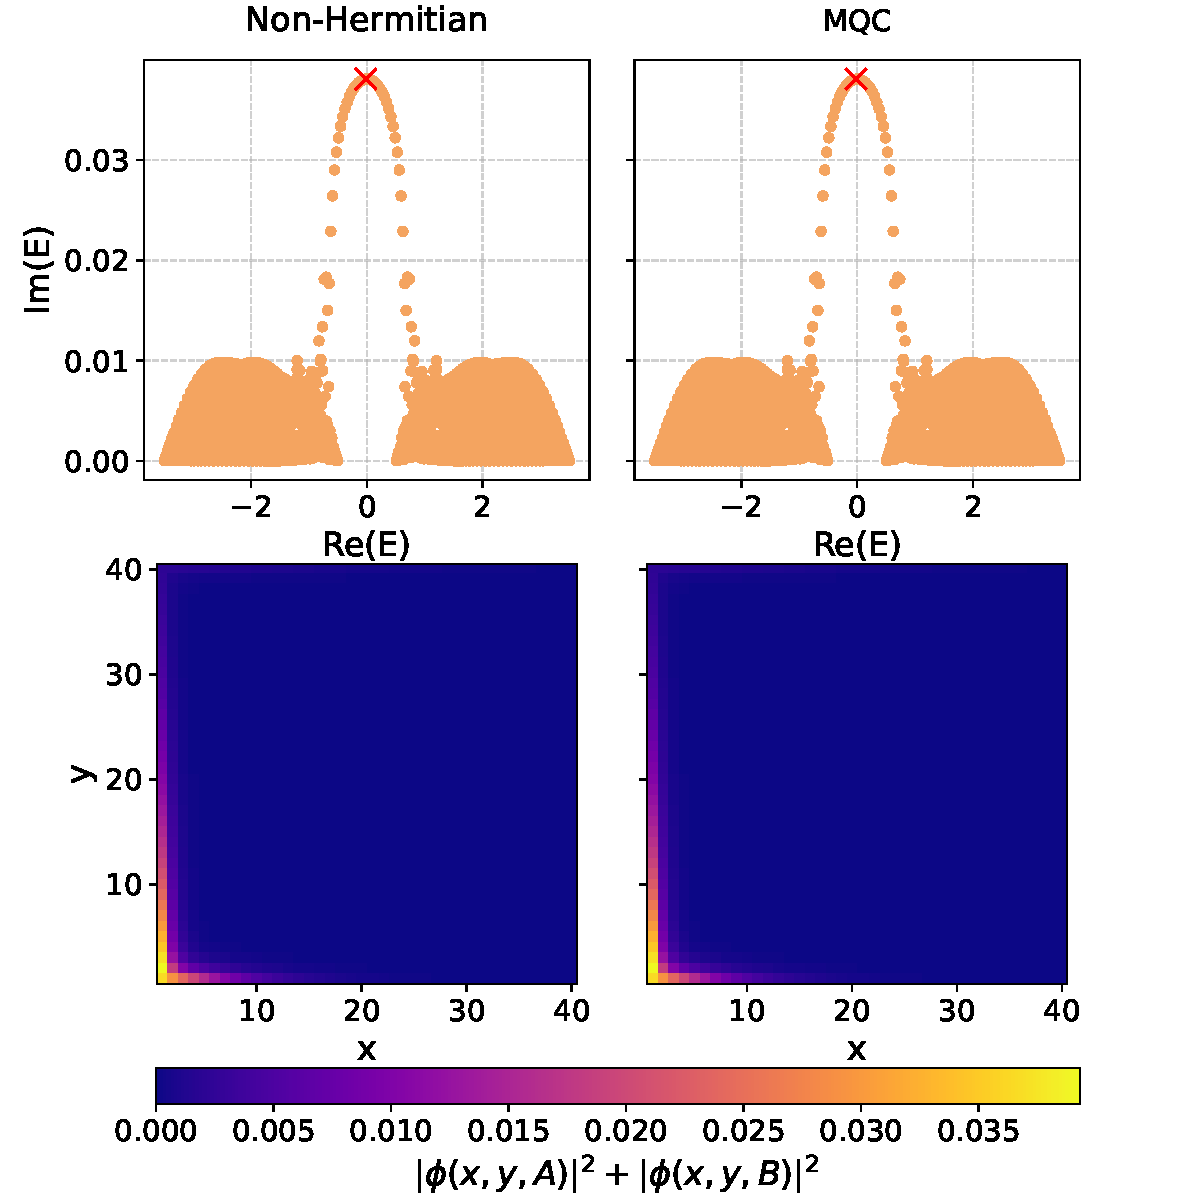
\includegraphics[width=1.\linewidth]{Picture/SingleExcitation_Comp.pdf}
		\caption{
		In the two-excitation subspace, the comparison of spectrum and eigenstates between the non-Hermitan Hamiltonian with or without $\hat{H}_{\text{inter}}$ many-body interaction. The Hermitian part is the three-dimensional chiral symmetric topological insulator. The non-Hermitian gain ($\gamma=0.2$) is applied on unit cells at the $z=1$ boundary.
		(a1) The spectrum of a non-Hermitian Hamiltonian without interaction.
		(b1) The spectrum of a non-Hermitian Hamiltonian with interaction.
		(a2) The probability distribution of the eigenstates of a non-Hermitian Hamiltonian without interaction. 
		(b2) The probability distribution of the eigenstates of a non-Hermitian Hamiltonian with interaction.
		(a3) The average particle number per lattice site for the eigenstate in (a2).
		(b3) The average particle number per lattice site for the eigenstate in (b2).
		The system size is $L_x=L_y=3,L_z=6$.
		}
		% \label{fig:13}
		\label{fig:16}
	\end{figure} %label from y=1 and x=1?

	% \section{The evolution of 4 excitations in the MQCs~\label{sec:appendF_4Body_Evolve}}
	% Here, we show the time evolution of multi-particles in the MQCs. The comparisons between the results of the MQC and exact time-evolution are given in Fig.~\ref{fig:18}. 
	% % 我们考虑一个$L_x=2,L_y=4$的二维晶格，耗散作用于$y=1$的边界上，相互作用部分为$U=1.0$的$\hat{H}_{\text{inter}}$，量子态初始的四个粒子分别位于元胞$(1,1)$和$(2,1)$的$A$格点和$B$格点。
	% % 在随后的时间对各个格点测量$\langle \hat{n}_{x,y,\alpha}\rangle$，相应的结果如图Fig.~\ref{fig:16}。它们分别是通过我们的方案的MQC和精确的方法对增益非厄米多体哈密顿量的模拟结果。它们之间的吻合表明我们的方案的MQC仅通过一个辅助比特能够对在更多粒子激发的非厄米多体哈密顿量进行模拟。
	% We consider a two-dimensional lattice whose size is $L_x = 2$, $L_y = 4$, and gain is applied at the unit cells of $y = 1$ boundary. The interaction term is $\hat{H}_{\text{inter}}$ with interaction strength $U_{\text{inter}} = 1.0$. The initial state contains four fermions located at the $A$ and $B$ sublattices of the $(1,1)$ and $(2,1)$ unit cells. We measure the average particle number $\langle \hat{n}(x,y,\alpha) \rangle$ at different time, as shown in Fig.~\ref{fig:18}. 
	% Both the simulation results obtained from our MQCs framework and the exact numerical calculations of the gain non-Hermitian many-body Hamiltonian exhibit excellent agreement (Fig.~\ref{fig:18}). This consistency demonstrates that our MQCs framework can faithfully reproduce the dynamics of non-Hermitian many-body systems.
	% \begin{figure}[h]
	% 	\centering
	% 	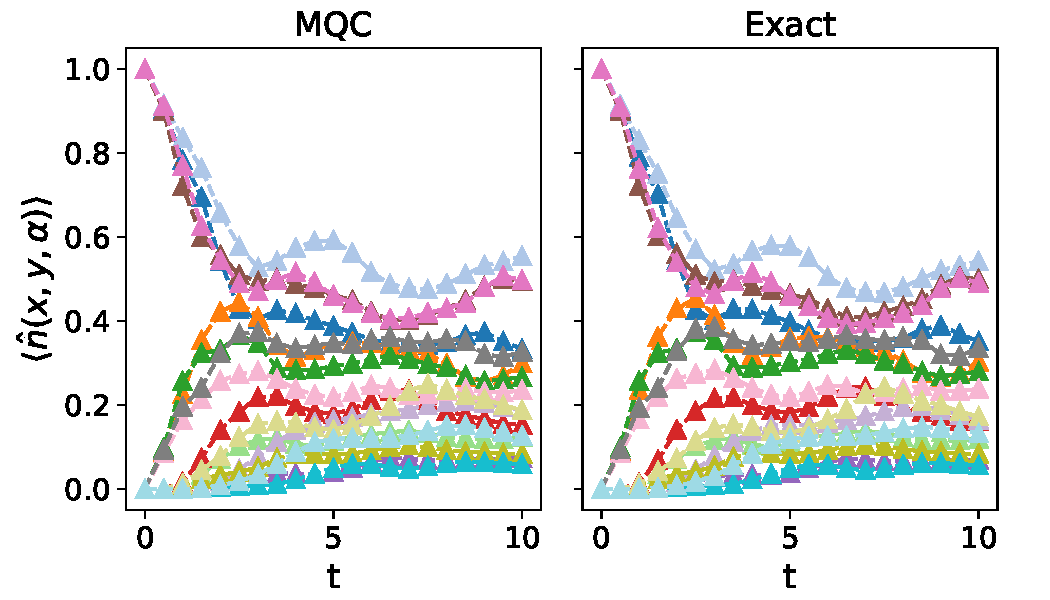
\includegraphics[width=1.\linewidth]{Picture/SI/SI_CircuitEvolve_4Body.pdf}
	% 	\caption{%从初始在元胞$(1,1)$和$(2,1)$的$A$子格点和$B$子格点各有一个粒子的四粒子态开始演化，在不同时间$t$不同格点的平均粒子数。分别是通过Fig.~\ref{fig:04}(a)的量子线路和精确计算得到的。系统尺寸为$L_x=2,L_y=4$，相互作用强度为$U_{\text{inter}}=1.0$，非厄米参数为$\gamma=0.2$。受控量子线路参数为$\mathrm{d}t=0.1$,$N=50$.
	% 	The average particle number for different lattice sites at time $t$. The $x$-axis is the time $t$.
	% 	The initial state consists of four fermions located at $(x,y,\alpha)=(1,1,A),(1,1,B),(2,1,A),(2,1,B)$. 
	% 	Results are obtained through both (a) the MQCs described in Fig.~\ref{fig:04}(a) and (b) the exact calculations. The system size is $L_x=2,L_y=4$. The interaction strength is $U_{\text{inter}} = 1.0$ and the non-Hermitian parameter is $\gamma = 0.2$. The parameters of the MQCs are $\mathrm{d}t = 0.1$ and $N = 100$.
	% 	}
	% 	\label{fig:18}
	% \end{figure}


	% If in two-column mode, this environment will change to single-column
	% format so that long equations can be displayed. Use
	% sparingly.
	%\begin{widetext}
	% put long equation here
	%\end{widetext}
	
	% figures should be put into the text as floats.
	% Use the graphics or graphicx packages (distributed with LaTeX2e)
	% and the \includegraphics macro defined in those packages.
	% See the LaTeX Graphics Companion by Michel Goosens, Sebastian Rahtz,
	% and Frank Mittelbach for instance.
	%
	% Here is an example of the general form of a figure:
	% Fill in the caption in the braces of the \caption{} command. Put the label
	% that you will use with \ref{} command in the braces of the \label{} command.
	% Use the figure* environment if the figure should span across the
	% entire page. There is no need to do explicit centering.
	
	% \begin{figure}
		% \includegraphics{}%
		% \caption{\label{}}
		% \end{figure}
	
	% Surround figure environment with turnpage environment for landscape
	% figure
	% \begin{turnpage}
		% \begin{figure}
			% \includegraphics{}%
			% \caption{\label{}}
			% \end{figure}
		% \end{turnpage}
	
	% tables should appear as floats within the text
	%
	% Here is an example of the general form of a table:
	% Fill in the caption in the braces of the \caption{} command. Put the label
	% that you will use with \ref{} command in the braces of the \label{} command.
	% Insert the column specifiers (l, r, c, d, etc.) in the empty braces of the
	% \begin{tabular}{} command.
		% The ruledtabular enviroment adds doubled rules to table and sets a
		% reasonable default table settings.
		% Use the table* environment to get a full-width table in two-column
		% Add \usepackage{longtable} and the longtable (or longtable*}
	% environment for nicely formatted long tables. Or use the the [H]
	% placement option to break a long table (with less control than 
	% in longtable).
	% \begin{table}%[H] add [H] placement to break table across pages
		% \caption{\label{}}
		% \begin{ruledtabular}
			% \begin{tabular}{}
				% Lines of table here ending with \\
				% \end{tabular}
			% \end{ruledtabular}
		% \end{table}
	
	% Surround table environment with turnpage environment for landscape
	% table
	% \begin{turnpage}
		% \begin{table}
			% \caption{\label{}}
			% \begin{ruledtabular}
				% \begin{tabular}{}
					% \end{tabular}
				% \end{ruledtabular}
			% \end{table}
		% \end{turnpage}
	
	% Specify following sections are appendices. Use \appendix* if there
	% only one appendix.
	%\appendix
	%\section{}
	
	% If you have acknowledgments, this puts in the proper section head.
	%\begin{acknowledgments}
	% put your acknowledgments here.
	%\end{acknowledgments}
	
	
	% Create the reference section using BibTeX:
	\bibliographystyle{apsrev4-1}
	%\bibliographystyle{unsrt}
	\bibliography{reference.bib}
	
\end{document}
%
% ****** End of file apstemplate.tex ******